% ══════════════════════════════════════════════════════════════════
\chapter{Methodology}
\label{ch:methodology}
% ══════════════════════════════════════════════════════════════════

This chapter details every component of the SCR Financial Networks framework: the data pipeline that constructs time-evolving graphs from market observables, the spectral coarse-graining procedure that reduces graph complexity while preserving dynamical properties, the GAT-LSTM architecture that learns to predict spectral evolution, the three-channel agent-based model that simulates contagion cascades, and the risk metrics that translate network diagnostics into quantitative indicators.


% ──────────────────────────────────────────────────────────────────
\section{System Architecture Overview}
\label{sec:architecture}
% ──────────────────────────────────────────────────────────────────

\begin{figure}[H]
    \centering
    \begin{tikzpicture}[
        box/.style={rectangle, rounded corners=5pt, draw=black!50, line width=1pt, minimum height=1.8cm, text width=4.0cm, align=center, font=\small},
        widebox/.style={rectangle, rounded corners=5pt, draw=black!50, line width=1pt, minimum height=1.5cm, text width=10cm, align=center, font=\small},
        arr/.style={-{Stealth[length=7pt]}, line width=1.2pt, draw=black!40},
    ]
    % Row 1: Data sources
    \node[box, fill=blue!10] (yf) at (0,0) {\textbf{yfinance API}\\[3pt]\footnotesize 10 bank stocks\\[-1pt]\footnotesize Daily OHLCV (2021--2024)};
    \node[box, fill=blue!10] (ecb) at (6.5,0) {\textbf{ECB SDW}\\[3pt]\footnotesize Sovereign 10Y yields\\[-1pt]\footnotesize (IT, DE, FR, ES, NL, SE)};

    % Row 2: Network construction
    \node[widebox, fill=green!10] (net) at (3.25,-2.5) {\textbf{Network Construction}\\[3pt]\footnotesize Rolling Pearson correlation (60-day window)\\[-1pt]\footnotesize Threshold filtering at $\rho_{\min}=0.3$};

    \draw[arr] (yf.south) -- (yf.south |- net.north);
    \draw[arr] (ecb.south) -- (ecb.south |- net.north);

    % Row 3: Three pipelines (absolute positions for clean spacing)
    \node[box, fill=red!8] (scg) at (-2.5,-5.5) {\textbf{SCG Pipeline}\\[3pt]\footnotesize Eigendecomposition\\[-1pt]\footnotesize ER gap test ($p<0.01$)\\[-1pt]\footnotesize Coarse-grain \& rescale\\[-1pt]\footnotesize Diffusion validation};
    \node[box, fill=blue!6] (gat) at (3.25,-5.5) {\textbf{GAT-LSTM Predictor}\\[3pt]\footnotesize GATConv ($K{=}8$ heads)\\[-1pt]\footnotesize BatchNorm + ELU\\[-1pt]\footnotesize LSTM (2 layers)\\[-1pt]\footnotesize $\to[\lambda_2,\;\delta,\;\rho]$};
    \node[box, fill=purple!8] (abm) at (9,-5.5) {\textbf{3-Channel ABM}\\[3pt]\footnotesize 1.\ Credit contagion\\[-1pt]\footnotesize 2.\ Funding liquidity\\[-1pt]\footnotesize 3.\ Fire-sale losses\\[-1pt]\footnotesize Monte Carlo (100 runs)};

    % Angled arrows from net to each pipeline
    \draw[arr] (net.south) -- (scg.north);
    \draw[arr] (net.south) -- (gat.north);
    \draw[arr] (net.south) -- (abm.north);

    % Row 4: Risk metrics
    \node[widebox, fill=yellow!12] (risk) at (3.25,-8.5) {\textbf{Risk Metrics}\\[3pt]\footnotesize SRISK, MES, CoVaR, VaR, $\Delta$-CoVaR\\[-1pt]\footnotesize SCG Risk $= 1 - \lambda_2/\rho$};

    \draw[arr] (scg.south) -- (scg.south |- risk.north);
    \draw[arr] (gat.south) -- (risk.north);
    \draw[arr] (abm.south) -- (abm.south |- risk.north);

    % Row 5: Dashboard
    \node[widebox, fill=orange!12] (dash) at (3.25,-10.5) {\textbf{Interactive Dashboard}\\[3pt]\footnotesize Dash + FastAPI: Network $\cdot$ Simulate $\cdot$ Spectral $\cdot$ Evolve $\cdot$ AI/Data};

    \draw[arr] (risk.south) -- (dash.north);
    \end{tikzpicture}
    \caption{System architecture of the SCR Financial Networks framework. Market data flows from Yahoo Finance and the ECB Statistical Data Warehouse through a rolling correlation pipeline that produces daily weighted adjacency matrices. These feed into three analytical modules---spectral coarse-graining (SCG), a temporal Graph Attention Network (GAT-LSTM), and a three-channel agent-based model (ABM)---whose outputs are integrated through a risk metrics layer and visualised via an interactive Dash dashboard served by FastAPI.}
    \label{fig:architecture}
\end{figure}

The framework (Figure~\ref{fig:architecture}) is organised as a directed acyclic graph of computation stages. Raw market data enters through two external APIs---Yahoo Finance for bank stock prices and the ECB Statistical Data Warehouse for sovereign yields and macroeconomic indicators. A preprocessing stage computes rolling log-return correlations and constructs weighted adjacency matrices with configurable threshold filtering. These daily graph snapshots then flow into three parallel analysis pipelines:

\begin{enumerate}[label=(\roman*)]
    \item \textbf{Spectral Coarse-Graining}: reduces the $N$-node graph to a smaller graph of $K < N$ super-nodes that preserves diffusion dynamics, using the Erd\H{o}s--R\'{e}nyi null model gap test~\cite{schmidt2024spectral} to determine the optimal reduction dimension.
    \item \textbf{GAT-LSTM Predictor}: ingests sequences of graph snapshots and predicts future values of three spectral targets---algebraic connectivity $\lambda_2$, spectral radius $\rho$, and spectral gap $\delta$.
    \item \textbf{Three-Channel ABM}: simulates contagion cascades through credit, funding, and fire-sale channels, with initial conditions drawn from observed network states.
\end{enumerate}

A risk metrics module aggregates outputs from all three pipelines, computing standard systemic risk measures (SRISK, MES, CoVaR) alongside the novel SCG-based indicator. An interactive dashboard provides real-time visualisation and parameter exploration.


% ──────────────────────────────────────────────────────────────────
\section{Data Pipeline and Network Construction}
\label{sec:data-pipeline}
% ──────────────────────────────────────────────────────────────────

\subsection{Bank Selection Rationale}

We construct a 10-bank European interbank network designed to capture the dominant channels of cross-border financial contagion within the European banking system. The sample was selected according to three criteria: (i)~\emph{geographic diversity}---banks from 8 countries spanning the Eurozone core (Germany, France, Netherlands), periphery (Spain, Italy), Nordics (Sweden), and non-Eurozone centres (Switzerland, United Kingdom); (ii)~\emph{systemic importance}---all 10 institutions appear on the Financial Stability Board's list of Global Systemically Important Banks (G-SIBs) or are classified as Other Systemically Important Institutions (O-SIIs) by national authorities; (iii)~\emph{data availability}---all stocks have liquid, continuously traded equities with complete daily price histories over the analysis period.

\begin{table}[H]
\centering
\caption{Bank sample with node identifiers, ticker symbols, and home countries. Internal identifiers follow the format \texttt{CC\_XXX} where \texttt{CC} is the ISO~3166-1 country code and \texttt{XXX} is an abbreviated institution name.}
\label{tab:banks}
\begin{tabular}{lllll}
\toprule
\textbf{Node ID} & \textbf{Bank} & \textbf{Ticker} & \textbf{Country} & \textbf{Total Assets (bn EUR)} \\
\midrule
DE\_DBK  & Deutsche Bank      & DBK.DE    & Germany       & 1,312 \\
FR\_BNP  & BNP Paribas        & BNP.PA    & France        & 2,591 \\
ES\_SAN  & Santander          & SAN.MC    & Spain         & 1,849 \\
IT\_UCG  & UniCredit          & UCG.MI    & Italy         & 874 \\
NL\_ING  & ING Group          & INGA.AS   & Netherlands   & 992 \\
SE\_NDA  & Nordea             & NDA-SE.ST & Sweden        & 571 \\
CH\_UBS  & UBS                & UBSG.SW   & Switzerland   & 1,718 \\
UK\_BARC & Barclays           & BARC.L    & United Kingdom & 1,514 \\
UK\_HSBC & HSBC               & HSBA.L    & United Kingdom & 2,989 \\
FR\_ACA  & Cr\'{e}dit Agricole & ACA.PA   & France        & 2,379 \\
\bottomrule
\end{tabular}
\end{table}

The sample contains the two largest European banks by total assets (HSBC at EUR~2,989~bn, BNP~Paribas at EUR~2,591~bn), ensuring that the network captures systemically relevant interconnections. The inclusion of two UK banks and two French banks permits intra-country correlation analysis, while the geographic spread enables examination of cross-border contagion pathways.

\subsection{Data Sources and Retrieval}

Daily adjusted closing prices are retrieved via the \texttt{yfinance} Python API for the period 1~January~2021 to 31~December~2024, yielding $T = 1{,}096$ trading days after removing weekends and public holidays. Sovereign yield curves are obtained from the ECB Statistical Data Warehouse (SDW) using the \texttt{ecb-data} API wrapper. Both sources are freely available for academic research and require no authentication.

For each trading day $t$, we compute the log-return of bank $i$ as:
\begin{equation}
    r_{i,t} = \ln\!\left(\frac{P_{i,t}}{P_{i,t-1}}\right)
    \label{eq:logreturn}
\end{equation}
where $P_{i,t}$ is the adjusted closing price of bank $i$ at time $t$.

\subsection{Correlation Matrix Computation}

We compute the pairwise Pearson correlation of log-returns over a rolling window of $w = 60$ trading days (approximately 3 calendar months). For banks $i$ and $j$ at time $t$, the rolling correlation is:
\begin{equation}
    \rho_{ij}(t) = \frac{\sum_{s=t-w+1}^{t} \left(r_{i,s} - \bar{r}_i(t)\right)\left(r_{j,s} - \bar{r}_j(t)\right)}{\sqrt{\sum_{s=t-w+1}^{t}\left(r_{i,s} - \bar{r}_i(t)\right)^2 \cdot \sum_{s=t-w+1}^{t}\left(r_{j,s} - \bar{r}_j(t)\right)^2}}
    \label{eq:pearson}
\end{equation}
where $\bar{r}_i(t) = \frac{1}{w}\sum_{s=t-w+1}^{t} r_{i,s}$ is the rolling mean return. The window size $w=60$ balances responsiveness to regime changes against estimation noise from short samples~\cite{laloux1999noise,mantegna1999introduction}.

\subsection{Threshold Filtering and Adjacency Matrix}

The raw correlation matrix $\rho(t) \in [-1, 1]^{N \times N}$ is converted into a weighted adjacency matrix $A(t)$ by applying a threshold $\rho_{\min}$:
\begin{equation}
    A_{ij}(t) = \begin{cases}
        \rho_{ij}(t) & \text{if } i \neq j \text{ and } \rho_{ij}(t) \geq \rho_{\min} \\
        0 & \text{otherwise}
    \end{cases}
    \label{eq:threshold}
\end{equation}

The threshold $\rho_{\min}$ controls the trade-off between network density and signal-to-noise ratio. Lower thresholds retain more edges but include weak, potentially spurious correlations; higher thresholds produce sparser, more informative graphs but may disconnect the network. We use $\rho_{\min} = 0.3$ as the default, yielding a mean density of $0.907$ with $41 \pm 6$ edges (Table~\ref{tab:threshold}), and conduct a full sensitivity analysis in Section~\ref{sec:threshold-sensitivity}. The choice is motivated by the observation that correlations below $0.3$ among major European bank stocks are typically indistinguishable from noise at conventional significance levels.

\subsection{Node Feature Computation}
\label{sec:node-features}

Each node $i$ at time $t$ is assigned a feature vector $\mathbf{x}_i(t) \in \mathbb{R}^5$ comprising five financial indicators:

\begin{enumerate}
    \item \textbf{Rolling volatility}: the annualised standard deviation of log-returns over the past $w=60$ days:
    \begin{equation}
        \sigma_i(t) = \sqrt{252} \cdot \sqrt{\frac{1}{w-1}\sum_{s=t-w+1}^{t}\left(r_{i,s} - \bar{r}_i(t)\right)^2}
        \label{eq:volatility}
    \end{equation}
    where the factor $\sqrt{252}$ annualises from daily to yearly.

    \item \textbf{Cumulative return}: the total return over the rolling window:
    \begin{equation}
        R_i(t) = \sum_{s=t-w+1}^{t} r_{i,s}
        \label{eq:cumreturn}
    \end{equation}

    \item \textbf{Degree centrality}: the fraction of possible edges realised after thresholding:
    \begin{equation}
        d_i(t) = \frac{1}{N-1}\sum_{j \neq i} \mathbf{1}\!\left[A_{ij}(t) > 0\right]
        \label{eq:degree}
    \end{equation}

    \item \textbf{Strength centrality}: the sum of edge weights incident on node $i$:
    \begin{equation}
        s_i(t) = \sum_{j \neq i} A_{ij}(t)
        \label{eq:strength}
    \end{equation}

    \item \textbf{Eigenvector centrality}: the $i$-th component of the leading eigenvector of $A(t)$, normalised to unit $\ell_2$ norm. This is the unique positive vector satisfying:
    \begin{equation}
        A(t)\,\mathbf{v}_1 = \lambda_1 \,\mathbf{v}_1, \qquad \|\mathbf{v}_1\| = 1
        \label{eq:eigenvec}
    \end{equation}
    by the Perron--Frobenius theorem~\cite{golub2013matrix}.
\end{enumerate}

All features are standardised to zero mean and unit variance across the node dimension at each time step, preventing scale differences from biasing the GAT attention mechanism.

\subsection{Spectral Target Computation}

The GAT-LSTM is trained to predict three spectral properties of the graph at time $t$:

\begin{enumerate}
    \item \textbf{Algebraic connectivity} ($\lambda_2$): the second-smallest eigenvalue of the graph Laplacian $L(t) = D(t) - A(t)$, where $D(t) = \mathrm{diag}(s_1(t), \ldots, s_N(t))$ is the degree matrix~\cite{fiedler1973algebraic}. This quantifies the bottleneck connectivity of the network; $\lambda_2 = 0$ if and only if the graph is disconnected.

    \item \textbf{Spectral radius} ($\rho$): the largest eigenvalue of $A(t)$ in absolute value. For non-negative matrices, $\rho = \lambda_1$ by the Perron--Frobenius theorem. The spectral radius governs the rate of diffusion spread and is an upper bound on mean node degree~\cite{cvetkovic1995spectra}.

    \item \textbf{Spectral gap} ($\delta$): the difference between the two largest eigenvalues of $A(t)$:
    \begin{equation}
        \delta(t) = \lambda_1(t) - \lambda_2^{(A)}(t)
        \label{eq:gap}
    \end{equation}
    where $\lambda_1$ and $\lambda_2^{(A)}$ are eigenvalues of the adjacency matrix (not the Laplacian). A large gap indicates strong community structure and rapid mixing~\cite{chung1997spectral}.
\end{enumerate}

These three targets are computed from the full Laplacian and adjacency eigenspectra at each snapshot. For the empirical dataset, the daily means are: $\lambda_2 = 0.923 \pm 0.160$, $\rho = 5.36 \pm 0.58$, and spectral gap $\delta = 0.24 \pm 0.18$ (Section~\ref{sec:spectral-evolution}).


% ──────────────────────────────────────────────────────────────────
\section{Spectral Coarse-Graining Implementation}
\label{sec:scg-method}
% ──────────────────────────────────────────────────────────────────

Spectral coarse-graining (SCG) is a graph renormalization procedure that reduces a graph $G$ with $N$ nodes to a coarse-grained graph $\tilde{G}$ with $K < N$ super-nodes, while provably preserving diffusion dynamics on the graph~\cite{schmidt2024spectral}. The procedure generalises the real-space renormalization group from statistical physics~\cite{wilson1975renormalization} to arbitrary network topologies, building on the observation that low-frequency eigenmodes of the graph Laplacian capture the dominant mesoscale structure~\cite{villegas2023laplacian}.

\subsection{Mathematical Foundation}

Let $G = (V, E, W)$ be a weighted undirected graph with $N = |V|$ nodes and symmetric adjacency matrix $A \in \mathbb{R}^{N \times N}$. The \emph{combinatorial Laplacian} is $L = D - A$ where $D = \mathrm{diag}(d_1, \ldots, d_N)$ and $d_i = \sum_j A_{ij}$. The \emph{normalised Laplacian} is $\mathcal{L} = D^{-1/2} L \, D^{-1/2}$, with eigenvalues $0 = \mu_1 \leq \mu_2 \leq \cdots \leq \mu_N$~\cite{chung1997spectral}.

\begin{definition}[Spectral Coarse-Graining]
Given a graph $G$ with Laplacian eigenpairs $\{(\lambda_k, \mathbf{u}_k)\}_{k=1}^N$ and a partition $\mathcal{P} = \{C_1, \ldots, C_K\}$ of $V$ into $K$ groups, the coarse-grained Laplacian is:
\begin{equation}
    \tilde{L} = P^T L P \left(P^T P\right)^{-1}
    \label{eq:scg-laplacian}
\end{equation}
where $P \in \{0,1\}^{N \times K}$ is the partition indicator matrix with $P_{ik} = 1$ if node $i \in C_k$.
\end{definition}

The key property is that SCG preserves the action of the heat kernel: if $\mathbf{f}(t) = e^{-tL}\mathbf{f}(0)$ is a diffusion process on $G$, then the coarse-grained process $\tilde{\mathbf{f}}(t) = e^{-t\tilde{L}}\tilde{\mathbf{f}}(0)$ approximates the group-averaged dynamics of $\mathbf{f}(t)$ with error bounded by the discarded eigenvalues~\cite{schmidt2024spectral}.

\subsection{Six-Step SCG Procedure}

The complete SCG pipeline proceeds as follows:

\paragraph{Step 1: Laplacian Type Detection.}
The algorithm automatically selects between the combinatorial Laplacian $L$ and the normalised Laplacian $\mathcal{L}$ based on degree heterogeneity. Defining the coefficient of variation of the degree sequence as:
\begin{equation}
    \mathrm{CV}(d) = \frac{\mathrm{std}(d_1, \ldots, d_N)}{\mathrm{mean}(d_1, \ldots, d_N)}
    \label{eq:cv-degree}
\end{equation}
we use the normalised Laplacian $\mathcal{L}$ when $\mathrm{CV}(d) > 0.5$ (heterogeneous degree distributions, e.g., scale-free networks) and the combinatorial Laplacian $L$ otherwise (approximately regular networks). This heuristic is motivated by the fact that the normalised Laplacian produces more interpretable spectra for networks with high degree variance~\cite{luxburg2007tutorial}.

\paragraph{Step 2: Eigendecomposition.}
Compute the full eigendecomposition $L = U \Lambda U^T$ where $\Lambda = \mathrm{diag}(\lambda_1, \ldots, \lambda_N)$ and $U = [\mathbf{u}_1 | \cdots | \mathbf{u}_N]$ is the matrix of orthonormal eigenvectors.

\paragraph{Step 3: Gap Test via Erd\H{o}s--R\'{e}nyi Null Model.}
To determine the number of coarse-grained groups $K$, we identify statistically significant gaps in the Laplacian spectrum by comparing with a null distribution. The null model is an Erd\H{o}s--R\'{e}nyi (ER) random graph $G(N, p)$ with the same expected density as the observed graph. Algorithm~\ref{alg:gaptest} details this procedure.

\begin{algorithm}[H]
\caption{Erd\H{o}s--R\'{e}nyi Spectral Gap Test}
\label{alg:gaptest}
\begin{algorithmic}[1]
\Require Graph $G$ with $N$ nodes and edge density $\hat{p}$; number of null samples $M = 500$; significance level $\alpha = 0.01$
\Ensure Number of groups $K$; significant gap positions
\State Compute Laplacian eigenvalues $\lambda_1 \leq \lambda_2 \leq \cdots \leq \lambda_N$ of $G$
\State Compute consecutive gaps: $g_k = \lambda_{k+1} - \lambda_k$ for $k = 1, \ldots, N-1$
\For{$m = 1, \ldots, M$}
    \State Generate ER graph $G_m \sim G(N, \hat{p})$ with density $\hat{p}$
    \State Compute Laplacian eigenvalues $\lambda_1^{(m)} \leq \cdots \leq \lambda_N^{(m)}$ of $G_m$
    \State Record gaps: $g_k^{(m)} = \lambda_{k+1}^{(m)} - \lambda_k^{(m)}$ for $k = 1, \ldots, N-1$
\EndFor
\For{$k = 1, \ldots, N-1$}
    \State Compute $p$-value: $p_k = \frac{1}{M}\sum_{m=1}^{M} \mathbf{1}[g_k^{(m)} \geq g_k]$
\EndFor
\State Let $k^* = \min\{k : p_k < \alpha\}$ be the first significant gap position
\State \Return $K = k^*$; gap positions $\{k : p_k < \alpha\}$
\end{algorithmic}
\end{algorithm}

The gap test formalises the intuition that a ``true'' spectral gap---indicating genuine mesoscale structure---should be statistically improbable under a structureless null model. We use $M = 500$ null samples and a significance level $\alpha = 0.01$, with Bonferroni correction applied across the $N-1$ tests~\cite{schmidt2024spectral}.

\paragraph{Step 4: Eigenvector Clustering.}
Given $K$ groups, we cluster nodes using the first $K$ non-trivial eigenvectors of the Laplacian. Following the spectral clustering methodology of Ng et al.~\cite{ng2002spectral}, we form the matrix $\hat{U} = [\mathbf{u}_2 | \cdots | \mathbf{u}_{K+1}] \in \mathbb{R}^{N \times K}$, row-normalise to the unit sphere, and apply $k$-means clustering with $K$ centres. The resulting partition $\mathcal{P} = \{C_1, \ldots, C_K\}$ minimises the normalised cut objective:
\begin{equation}
    \text{NCut}(\mathcal{P}) = \sum_{k=1}^{K} \frac{\text{cut}(C_k, \bar{C}_k)}{\text{vol}(C_k)}
    \label{eq:ncut}
\end{equation}
where $\text{cut}(C_k, \bar{C}_k) = \sum_{i \in C_k, j \notin C_k} A_{ij}$ and $\text{vol}(C_k) = \sum_{i \in C_k} d_i$~\cite{luxburg2007tutorial}.

\paragraph{Step 5: Coarse-Grained Graph Construction.}
The partition matrix $P \in \{0,1\}^{N \times K}$ defines the coarse-grained Laplacian via Equation~\eqref{eq:scg-laplacian}. The coarse-grained adjacency matrix is recovered as:
\begin{equation}
    \tilde{A} = \tilde{D} - \tilde{L}, \qquad \tilde{D} = \mathrm{diag}(\tilde{d}_1, \ldots, \tilde{d}_K)
    \label{eq:scg-adj}
\end{equation}
where $\tilde{d}_k = \sum_{l} \tilde{L}_{kl}$ for $k \neq l$ (since $\tilde{L}$ has zero row sums by construction).

\paragraph{Step 6: Validation.}
Quality is assessed by comparing diffusion dynamics on the original and coarse-grained graphs. We simulate the heat kernel $\mathbf{f}(t) = e^{-tL}\mathbf{f}(0)$ for $t \in [0, 10]$ with random initial conditions and measure preservation using three metrics:

\begin{enumerate}
    \item \textbf{Diffusion $R^2$}: the coefficient of determination between the group-averaged original dynamics and the coarse-grained dynamics, computed over all time steps:
    \begin{equation}
        R^2 = 1 - \frac{\sum_{k,t} \left(\bar{f}_k(t) - \tilde{f}_k(t)\right)^2}{\sum_{k,t} \left(\bar{f}_k(t) - \langle \bar{f} \rangle\right)^2}
        \label{eq:r2-diffusion}
    \end{equation}
    where $\bar{f}_k(t) = |C_k|^{-1}\sum_{i \in C_k} f_i(t)$ is the group average.

    \item \textbf{Eigenvalue RMSE}: the root-mean-square error between the first $K$ eigenvalues of $L$ and $\tilde{L}$:
    \begin{equation}
        \text{RMSE}_\lambda = \sqrt{\frac{1}{K}\sum_{k=1}^{K}\left(\lambda_k - \tilde{\lambda}_k\right)^2}
        \label{eq:rmse-eigenval}
    \end{equation}

    \item \textbf{Spectral fidelity}: the fraction of eigenvalue variance preserved by the coarse-grained spectrum.
\end{enumerate}


% ──────────────────────────────────────────────────────────────────
\section{GAT-LSTM Architecture}
\label{sec:gat-architecture}
% ──────────────────────────────────────────────────────────────────

The temporal prediction module combines a Graph Attention Network (GAT) encoder~\cite{velickovic2018graph} with a Long Short-Term Memory (LSTM) network~\cite{hochreiter1997long} to learn representations from sequences of graph snapshots and predict spectral target evolution.

\subsection{GAT Encoder}

The GAT encoder processes a single graph snapshot $G_t = (V, E_t, A_t, X_t)$ where $X_t \in \mathbb{R}^{N \times F}$ is the node feature matrix with $F = 5$ features per node (Section~\ref{sec:node-features}).

\paragraph{Attention Mechanism.}
For a pair of connected nodes $(i, j) \in E_t$, the unnormalised attention coefficient in layer $\ell$ is:
\begin{equation}
    e_{ij}^{(\ell)} = \mathrm{LeakyReLU}\!\left(\mathbf{a}^{(\ell)\top}\left[W^{(\ell)}\mathbf{h}_i^{(\ell-1)} \,\|\, W^{(\ell)}\mathbf{h}_j^{(\ell-1)}\right]\right)
    \label{eq:gat-attention}
\end{equation}
where $W^{(\ell)} \in \mathbb{R}^{F' \times F^{(\ell-1)}}$ is a learnable weight matrix, $\mathbf{a}^{(\ell)} \in \mathbb{R}^{2F'}$ is the attention parameter vector, $\|$ denotes concatenation, and LeakyReLU uses negative slope $0.2$~\cite{velickovic2018graph}. Attention is normalised over the neighbourhood $\mathcal{N}(i)$ of node $i$ using softmax:
\begin{equation}
    \alpha_{ij}^{(\ell)} = \frac{\exp(e_{ij}^{(\ell)})}{\sum_{k \in \mathcal{N}(i)} \exp(e_{ik}^{(\ell)})}
    \label{eq:gat-softmax}
\end{equation}

\paragraph{Multi-Head Attention.}
Each GAT layer employs $K$ independent attention heads. The output of layer $\ell$ for node $i$ is:
\begin{equation}
    \mathbf{h}_i^{(\ell)} = \text{ELU}\!\left(\frac{1}{K}\sum_{k=1}^{K}\sum_{j \in \mathcal{N}(i)} \alpha_{ij}^{(\ell,k)} W^{(\ell,k)} \mathbf{h}_j^{(\ell-1)}\right)
    \label{eq:gat-multihead}
\end{equation}
where the heads are averaged (rather than concatenated) in intermediate layers, and ELU is the Exponential Linear Unit activation. We found averaging to produce more stable training than concatenation for our small graphs, consistent with observations in Veli\v{c}kovi\'{c} et al.~\cite{velickovic2018graph}.

\paragraph{Batch Normalisation and Dropout.}
Each GAT layer is followed by BatchNorm~\cite{goodfellow2016deep} applied to the node feature dimension, then dropout with probability $p_{\text{drop}} = 0.1$. For the regularised configuration, dropout is increased to $p_{\text{drop}} = 0.3$ and weight decay is applied.

\subsection{Graph Readout}

After the final GAT layer, we obtain a set of node embeddings $\{\mathbf{h}_i^{(L)}\}_{i=1}^{N}$ where $L$ is the number of GAT layers. We use mean pooling as the graph-level readout:
\begin{equation}
    \mathbf{z}_t = \frac{1}{N}\sum_{i=1}^{N} \mathbf{h}_i^{(L)} \in \mathbb{R}^{d_{\text{hidden}}}
    \label{eq:readout}
\end{equation}
where $d_{\text{hidden}}$ is the hidden dimension of the final GAT layer. Mean pooling was chosen over more expressive alternatives (e.g., attention-based readout, Set2Set) because the fixed node set and small graph size ($N=10$) make permutation-equivariant readout sufficient, and preliminary experiments showed no benefit from more complex pooling.

\subsection{LSTM Temporal Module}

The graph-level embeddings $\mathbf{z}_1, \ldots, \mathbf{z}_T$ from $T$ consecutive graph snapshots are processed by a single-layer LSTM to capture temporal dependencies. The LSTM hidden state equations are:
\begin{align}
    \mathbf{f}_t &= \sigma\!\left(W_f [\mathbf{z}_t \,\|\, \mathbf{h}_{t-1}] + \mathbf{b}_f\right) \label{eq:lstm-forget}\\
    \mathbf{i}_t &= \sigma\!\left(W_i [\mathbf{z}_t \,\|\, \mathbf{h}_{t-1}] + \mathbf{b}_i\right) \label{eq:lstm-input}\\
    \tilde{\mathbf{c}}_t &= \tanh\!\left(W_c [\mathbf{z}_t \,\|\, \mathbf{h}_{t-1}] + \mathbf{b}_c\right) \label{eq:lstm-candidate}\\
    \mathbf{c}_t &= \mathbf{f}_t \odot \mathbf{c}_{t-1} + \mathbf{i}_t \odot \tilde{\mathbf{c}}_t \label{eq:lstm-cell}\\
    \mathbf{o}_t &= \sigma\!\left(W_o [\mathbf{z}_t \,\|\, \mathbf{h}_{t-1}] + \mathbf{b}_o\right) \label{eq:lstm-output}\\
    \mathbf{h}_t &= \mathbf{o}_t \odot \tanh(\mathbf{c}_t) \label{eq:lstm-hidden}
\end{align}
where $\sigma$ is the sigmoid function, $\odot$ denotes element-wise multiplication, and $\{W_f, W_i, W_c, W_o, \mathbf{b}_f, \mathbf{b}_i, \mathbf{b}_c, \mathbf{b}_o\}$ are learnable parameters. The LSTM hidden dimension matches $d_{\text{hidden}}$.

\subsection{Prediction Head}

The final LSTM hidden state $\mathbf{h}_T$ is passed through a two-layer MLP:
\begin{equation}
    \hat{\mathbf{y}} = W_2 \,\mathrm{ReLU}(W_1 \mathbf{h}_T + \mathbf{b}_1) + \mathbf{b}_2 \in \mathbb{R}^{3}
    \label{eq:mlp-head}
\end{equation}
where $W_1 \in \mathbb{R}^{d_{\text{hidden}} \times d_{\text{hidden}}}$, $W_2 \in \mathbb{R}^{3 \times d_{\text{hidden}}}$, and the three outputs correspond to predictions of $(\lambda_2, \rho, \delta)$ at the next time step.

\subsection{Training Protocol}

\paragraph{Loss Function.}
We minimise the mean squared error (MSE) between predicted and observed spectral targets:
\begin{equation}
    \mathcal{L} = \frac{1}{3}\sum_{j=1}^{3}\left(\hat{y}_j - y_j\right)^2
    \label{eq:mse-loss}
\end{equation}
where the equal weighting across targets assumes comparable importance. We experimented with inverse-variance weighting but found no significant improvement.

\paragraph{Optimiser and Scheduler.}
Training uses Adam~\cite{goodfellow2016deep} with initial learning rate $\eta = 10^{-3}$, $\beta_1 = 0.9$, $\beta_2 = 0.999$, and weight decay $10^{-4}$. A cosine annealing learning rate scheduler~\cite{goodfellow2016deep} reduces $\eta$ to $10^{-6}$ over the maximum number of epochs. Gradient norms are clipped to $\|\nabla\| \leq 1.0$ to prevent exploding gradients in the LSTM.

\paragraph{Temporal Train/Test Split.}
The 220 weekly snapshots (stride~$=5$ from 1,096 daily snapshots) are split chronologically: the first 80\% ($T_{\text{train}} = 176$) for training and validation, and the final 20\% ($T_{\text{test}} = 44$) for testing. Within the training set, a further 80/20 split is used for training/validation. Temporal ordering is preserved---no future information leaks into training---which is critical for financial time-series applications~\cite{mantegna1999introduction}.

\paragraph{Early Stopping.}
Training terminates when the validation loss fails to improve for 15 consecutive epochs. Algorithm~\ref{alg:earlystop} formalises the criterion.

\begin{algorithm}[H]
\caption{Early Stopping with Patience}
\label{alg:earlystop}
\begin{algorithmic}[1]
\Require Patience $p = 15$; minimum improvement $\delta_{\min} = 10^{-4}$
\State Initialise: best loss $\ell^* \gets \infty$; counter $c \gets 0$
\For{epoch $= 1, 2, \ldots, E_{\max}$}
    \State Train one epoch; compute validation loss $\ell_{\text{val}}$
    \If{$\ell_{\text{val}} < \ell^* - \delta_{\min}$}
        \State $\ell^* \gets \ell_{\text{val}}$; $c \gets 0$; save model checkpoint
    \Else
        \State $c \gets c + 1$
    \EndIf
    \If{$c \geq p$}
        \State Restore best checkpoint; \textbf{break}
    \EndIf
\EndFor
\end{algorithmic}
\end{algorithm}


% ──────────────────────────────────────────────────────────────────
\section{Three-Channel Agent-Based Model}
\label{sec:abm-method}
% ──────────────────────────────────────────────────────────────────

The ABM simulates contagion cascades through a network of $N$ bank agents, each characterised by a state vector that evolves via Ornstein--Uhlenbeck (OU) dynamics with shocks propagating through three distinct contagion channels~\cite{tesfatsion2006agent,nier2007network}.

\subsection{Agent State Vector}

Each bank $i$ at simulation step $t$ is described by the state vector:
\begin{equation}
    \mathbf{s}_i(t) = \left(\text{CET1}_i(t),\; \text{LCR}_i(t),\; \text{TA}_i(t),\; \text{status}_i(t)\right)
    \label{eq:agent-state}
\end{equation}
where $\text{CET1}_i$ is the Common Equity Tier~1 ratio (capital adequacy), $\text{LCR}_i$ is the Liquidity Coverage Ratio, $\text{TA}_i$ is total assets, and $\text{status}_i \in \{\text{active}, \text{defaulted}\}$.

\subsection{Ornstein--Uhlenbeck Dynamics}

Between contagion events, the CET1 ratio of each active bank evolves according to a discrete-time Ornstein--Uhlenbeck process:
\begin{equation}
    \text{CET1}_i(t+1) = \text{CET1}_i(t) + \theta_{\text{CET1}}\left(\mu_{\text{CET1}} - \text{CET1}_i(t)\right) + \sigma_{\text{CET1}} \,\epsilon_i(t)
    \label{eq:ou-cet1}
\end{equation}
where $\theta_{\text{CET1}} = 0.1$ is the mean-reversion speed, $\mu_{\text{CET1}} = 0.12$ is the long-run mean (12\% CET1, reflecting European bank averages post-Basel~III~\cite{admati2013fallacies}), $\sigma_{\text{CET1}} = 0.005$ is the volatility parameter, and $\epsilon_i(t) \sim \mathcal{N}(0,1)$ is an i.i.d.\ noise term. The CET1 ratio is clamped to $[0.02, 0.25]$ after each update to prevent unrealistic values.

The LCR follows an analogous OU process:
\begin{equation}
    \text{LCR}_i(t+1) = \text{LCR}_i(t) + \theta_{\text{LCR}}\left(\mu_{\text{LCR}} - \text{LCR}_i(t)\right) + \sigma_{\text{LCR}} \,\epsilon_i'(t)
    \label{eq:ou-lcr}
\end{equation}
with $\theta_{\text{LCR}} = 0.1$, $\mu_{\text{LCR}} = 1.5$ (150\% LCR, above the regulatory minimum of 100\%~\cite{drehmann2013model}), $\sigma_{\text{LCR}} = 0.05$, and clamping to $[0.3, 3.0]$.

The OU specification introduces a fundamental modelling choice: the mean-reversion mechanism represents the tendency of banks to restore capital and liquidity buffers through retained earnings and portfolio adjustment~\cite{admati2013fallacies}. The parameter $\theta$ controls how quickly this restoration occurs; at $\theta = 0.1$, the half-life of a deviation is approximately 7 simulation steps.

\subsection{Channel 1: Credit Contagion}

When bank $j$ defaults, all creditors suffer credit losses proportional to their bilateral exposure:
\begin{equation}
    L_i^{\text{credit}} = \text{TA}_j \times A_{ij} \times \text{LGD}
    \label{eq:credit-loss}
\end{equation}
where $A_{ij}$ is the (normalised) edge weight representing the exposure of bank $i$ to bank $j$, and $\text{LGD} = 0.45$ is the loss given default, consistent with the Basel~II foundation IRB approach and empirical recovery rates for unsecured interbank claims~\cite{glasserman2015contagion}. The loss is applied to bank $i$'s capital:
\begin{equation}
    \text{CET1}_i \gets \text{CET1}_i - \frac{L_i^{\text{credit}}}{\text{TA}_i}
    \label{eq:credit-impact}
\end{equation}

This channel implements the classical cascading default mechanism analysed by Eisenberg and Noe~\cite{elliott2014financial} and extended by Gai and Kapadia~\cite{gai2010contagion}.

\subsection{Channel 2: Funding Liquidity Stress}

When bank $j$ defaults or is under stress ($\text{CET1}_j < 0.08$), other banks may withdraw interbank funding. The withdrawal probability is modelled as a sigmoid function of the counterparty's capital position:
\begin{equation}
    p_{\text{withdraw}}(i, j) = \frac{1}{1 + \exp\!\left(k \cdot (\text{CET1}_j - c)\right)}
    \label{eq:funding-prob}
\end{equation}
where $k = 50$ controls the steepness of the withdrawal threshold and $c = 0.06$ is the critical CET1 level. When $\text{CET1}_j = c$, the withdrawal probability is exactly 50\%; below $c$, it rapidly approaches 100\%.

Each withdrawal reduces the affected bank's LCR:
\begin{equation}
    \text{LCR}_i \gets \text{LCR}_i - A_{ij} \times f_{\text{stress}}
    \label{eq:funding-impact}
\end{equation}
where $f_{\text{stress}} = 0.3$ is the funding stress multiplier. This channel captures the liquidity spirals described by Brunnermeier~\cite{brunnermeier2009market} and modelled in Gai et al.~\cite{gai2010contagion}, where counterparty credit concerns trigger funding dry-ups that force deleveraging.

\subsection{Channel 3: Fire-Sale Contagion}

Banks with depleted liquidity ($\text{LCR}_i < 1.0$) are forced to sell assets at a discount, imposing mark-to-market losses on banks holding correlated assets:
\begin{equation}
    L_i^{\text{fire}} = \text{TA}_i \times \min\!\left(\sum_{j \in \mathcal{D}} A_{ij} \times h \times \gamma,\; 0.15\right)
    \label{eq:firesale-loss}
\end{equation}
where $\mathcal{D}$ is the set of currently defaulted banks, $h = 0.02$ is the base haircut per correlated default, and $\gamma$ is the amplification factor:
\begin{equation}
    \gamma = 1 + \frac{(n_{\text{def}} - 1)(c_{\text{amp}} - 1)}{N - 1}
    \label{eq:amplification}
\end{equation}
with $n_{\text{def}} = |\mathcal{D}|$ and $c_{\text{amp}} = 3$ controlling the maximum amplification. The cap at 15\% prevents unrealistic total wipeouts. The fire-sale channel follows the mechanism described by Caccioli et al.~\cite{caccioli2015overlapping} and implemented in multi-layer contagion models~\cite{poledna2015economics,bardoscia2017distress}.

\subsection{Cascade Algorithm}

At each simulation step, the three channels execute sequentially in a fixed order that reflects the empirical timing of financial contagion:

\begin{algorithm}[H]
\caption{Three-Channel Contagion Cascade}
\label{alg:cascade}
\begin{algorithmic}[1]
\Require Network $G = (V, E, A)$; agent states $\{\mathbf{s}_i\}_{i=1}^N$; scenario shocks
\State Apply scenario-specific shocks to agent states
\State $\mathcal{D}_{\text{new}} \gets \emptyset$ \Comment{Newly defaulted banks}
\Repeat
    \State $\mathcal{D}_{\text{prev}} \gets \mathcal{D}_{\text{new}}$
    \For{each active bank $i$} \Comment{Channel 1: Credit}
        \State Compute $L_i^{\text{credit}}$ from Eq.~\eqref{eq:credit-loss} for all $j \in \mathcal{D}$
        \State Update $\text{CET1}_i$ via Eq.~\eqref{eq:credit-impact}
    \EndFor
    \For{each active bank $i$} \Comment{Channel 2: Funding}
        \For{each neighbour $j$ with $\text{CET1}_j < 0.08$}
            \State Draw $u \sim \mathrm{Uniform}(0,1)$
            \If{$u < p_{\text{withdraw}}(i,j)$}
                \State Update $\text{LCR}_i$ via Eq.~\eqref{eq:funding-impact}
            \EndIf
        \EndFor
    \EndFor
    \For{each active bank $i$ with $\text{LCR}_i < 1.0$} \Comment{Channel 3: Fire-sale}
        \State Compute $L_i^{\text{fire}}$ from Eq.~\eqref{eq:firesale-loss}
        \State $\text{CET1}_i \gets \text{CET1}_i - L_i^{\text{fire}}/\text{TA}_i$
    \EndFor
    \State $\mathcal{D}_{\text{new}} \gets \{i : \text{CET1}_i < 0.02 \text{ or } \text{LCR}_i < 0.3\}$ \Comment{Default condition}
    \State Update $\text{status}_i \gets \text{defaulted}$ for all $i \in \mathcal{D}_{\text{new}}$
\Until{$\mathcal{D}_{\text{new}} = \mathcal{D}_{\text{prev}}$} \Comment{Fixed-point convergence}
\end{algorithmic}
\end{algorithm}

The default condition is triggered when a bank's CET1 ratio falls below 2\% (point of non-viability) or its LCR falls below 30\% (severe liquidity crisis). These thresholds are calibrated to be below the regulatory minima (4.5\% CET1, 100\% LCR) but above zero, reflecting the observation that regulatory intervention typically occurs before complete insolvency~\cite{drehmann2013model}.


% ──────────────────────────────────────────────────────────────────
\section{Risk Metrics Implementation}
\label{sec:risk-metrics}
% ──────────────────────────────────────────────────────────────────

The framework computes five risk metrics that span market-based and network-based approaches.

\paragraph{SRISK (Systemic Risk Measure).}
Following Brownlees and Engle~\cite{brownlees2017srisk}, the systemic risk contribution of bank $i$ is:
\begin{equation}
    \text{SRISK}_i = k \cdot D_i - (1-k) \cdot W_i \cdot (1 - \text{LRMES}_i)
    \label{eq:srisk}
\end{equation}
where $D_i$ is total debt, $W_i$ is market capitalisation, $k = 0.08$ is the prudential capital ratio, and $\text{LRMES}_i$ is the long-run marginal expected shortfall (the expected equity loss conditional on a 40\% market decline over 6 months). A positive SRISK indicates the capital shortfall a bank would suffer in a systemic event.

\paragraph{Marginal Expected Shortfall (MES).}
The MES of bank $i$ on day $t$ is the expected return conditional on the market being in its left tail~\cite{acharya2017measuring}:
\begin{equation}
    \text{MES}_{i,t} = -\mathbb{E}\left[r_{i,t} \mid r_{m,t} \leq \text{VaR}_{q}(r_m)\right]
    \label{eq:mes}
\end{equation}
where $r_{m,t}$ is the market return and $q = 0.05$ is the tail probability. We estimate MES nonparametrically using the empirical distribution of returns over the rolling window.

\paragraph{CoVaR.}
Following Adrian and Brunnermeier's methodology~\cite{bisias2012survey}, the CoVaR of the system conditional on bank $i$ being in distress is:
\begin{equation}
    \Pr\left(r_m \leq \text{CoVaR}_{q|i} \mid r_i = \text{VaR}_q(r_i)\right) = q
    \label{eq:covar}
\end{equation}
The risk contribution $\Delta\text{CoVaR}_i = \text{CoVaR}_{q|i} - \text{CoVaR}_{q|\text{median}_i}$ measures the incremental systemic risk when bank $i$ moves from its median state to distress.

\paragraph{Value-at-Risk (VaR).}
The standard VaR at confidence level $1-q$ is:
\begin{equation}
    \text{VaR}_{q,i} = -F_{r_i}^{-1}(q)
    \label{eq:var}
\end{equation}
where $F_{r_i}^{-1}$ is the inverse CDF of the return distribution, estimated via the empirical quantile.

\paragraph{SCG-Risk Indicator.}
The novel indicator derived from spectral coarse-graining is:
\begin{equation}
    \text{SCG-Risk}(t) = 1 - \frac{\lambda_2(t)}{\rho(t)}
    \label{eq:scg-risk}
\end{equation}
where $\lambda_2$ is the algebraic connectivity and $\rho$ is the spectral radius, both computed from the graph at time $t$. The ratio $\lambda_2/\rho \in [0, 1]$ for connected graphs measures the relative connectivity: when $\lambda_2/\rho \to 0$ (high SCG-Risk), the graph has a bottleneck making it vulnerable to fragmentation; when $\lambda_2/\rho \to 1$ (low SCG-Risk), the graph is highly connected and robust to edge removal~\cite{fiedler1973algebraic,estrada2015first}. The empirical range of this indicator is $[0.036, 0.695]$ with mean $0.237 \pm 0.181$ (Section~\ref{sec:spectral-evolution}).


% ══════════════════════════════════════════════════════════════════
\chapter{Implementation}
\label{ch:implementation}
% ══════════════════════════════════════════════════════════════════

This chapter describes the software architecture, dashboard design, and reproducibility measures that support the experimental framework.


% ──────────────────────────────────────────────────────────────────
\section{Software Architecture}
\label{sec:software}
% ──────────────────────────────────────────────────────────────────

The framework is implemented as a modular Python package \texttt{scr\_financial} comprising six submodules, organised to enforce separation of concerns between data processing, analytical methods, and presentation.

\begin{table}[H]
\centering
\caption{Package structure with module responsibilities and key dependencies.}
\label{tab:modules}
\small
\begin{tabularx}{\textwidth}{lXl}
\toprule
\textbf{Module} & \textbf{Responsibility} & \textbf{Dependencies} \\
\midrule
\texttt{network} & Data pipeline, graph construction, spectral analysis & NetworkX, SciPy \\
\texttt{ml}      & GAT-LSTM model, training, evaluation & PyTorch, PyG~\cite{fey2019fast} \\
\texttt{abm}     & Agent-based model, scenario engine & NumPy, Pandas \\
\texttt{risk}    & Risk metrics (SRISK, MES, CoVaR, VaR) & SciPy \\
\texttt{backtesting} & Indicator evaluation, correlation analysis & Pandas, SciPy \\
\texttt{vae}     & Variational autoencoder experiments & PyTorch \\
\texttt{utils}   & Configuration, logging, seed management & PyYAML \\
\bottomrule
\end{tabularx}
\normalsize
\end{table}

The \texttt{network} module implements the full data pipeline from Section~\ref{sec:data-pipeline}, including \texttt{yfinance} API integration, rolling correlation computation, threshold filtering, and Laplacian eigendecomposition. The \texttt{ml} module provides the GAT-LSTM architecture from Section~\ref{sec:gat-architecture} using PyTorch Geometric~\cite{fey2019fast} for message-passing layers and standard PyTorch for the LSTM and MLP components. The \texttt{abm} module implements the three-channel contagion model from Section~\ref{sec:abm-method} in pure NumPy for performance, with vectorised OU updates and matrix-based exposure propagation.

Total code size is approximately 8,000 lines of Python, excluding tests and dashboard frontend code. The analytical core (\texttt{network}, \texttt{ml}, \texttt{abm}, \texttt{risk}) comprises approximately 4,500 lines.


% ──────────────────────────────────────────────────────────────────
\section{Dashboard}
\label{sec:dashboard}
% ──────────────────────────────────────────────────────────────────

The interactive dashboard is built with Plotly Dash for the frontend and FastAPI for the backend API, providing a web-based interface for exploring all framework components without writing code. The application is organised into five pages:

\begin{enumerate}
    \item \textbf{Network Page}: Visualises the current correlation graph with node positions determined by a force-directed layout. Users can adjust the correlation threshold $\rho_{\min}$ via a slider and observe real-time changes to network topology, density, and spectral properties. Node colours encode eigenvector centrality; edge widths encode correlation strength.

    \item \textbf{Simulate Page}: Provides the ABM stress-testing interface. Users select from seven predefined scenarios or define custom shocks (CET1 reduction, LCR reduction, number of initially shocked banks). The simulation runs in the backend and results are streamed to the frontend, displaying default cascades, capital trajectories, and summary statistics.

    \item \textbf{Spectral Page}: Displays the Laplacian eigenspectrum, the SCG coarse-grained graph with cluster assignments, and diffusion preservation diagnostics. Users can compare the eigenspectra of the original and coarse-grained graphs interactively.

    \item \textbf{Evolve Page}: Shows time-series evolution of spectral properties ($\lambda_2$, $\rho$, $\delta$, SCG-Risk) alongside market volatility and network density. Configurable rolling windows and threshold parameters enable sensitivity exploration.

    \item \textbf{AI/Data Page}: Integrates the GAT-LSTM training pipeline with live progress monitoring. Training runs execute in a background thread using Python's \texttt{threading} module, with the frontend polling for progress updates at 2-second intervals. Users can launch hyperparameter sweeps, view training curves, and inspect attention weight visualisations.
\end{enumerate}

The live GNN training feature deserves particular note. Background threading decouples the training loop from the Dash callback event loop, preventing long-running computations from blocking the UI. A shared state dictionary (protected by a threading lock) stores epoch-level metrics, which the frontend retrieves via periodic callbacks. This architecture enables training sessions lasting several minutes while maintaining dashboard responsiveness.


% ──────────────────────────────────────────────────────────────────
\section{Reproducibility}
\label{sec:reproducibility}
% ──────────────────────────────────────────────────────────────────

All experiments use fixed random seeds across four sources of randomness: Python's \texttt{random} module (seed 42), NumPy (seed 42), PyTorch CPU (seed 42), and PyTorch CUDA (seed 42). The \texttt{utils} module provides a \texttt{set\_all\_seeds()} function that initialises all four generators, plus sets the \texttt{PYTHONHASHSEED} environment variable and enables PyTorch deterministic mode (\texttt{torch.use\_deterministic\_algorithms(True)}).

The hyperparameter sweep (Section~\ref{sec:gat-sweep}) runs each configuration with 5 different seeds (42, 43, 44, 45, 46) to report mean and standard deviation. Experiment configurations are stored as YAML files in an \texttt{experiments/} directory, and a runner script (\texttt{run\_experiments.py}) executes all configurations sequentially, logging results to structured JSON files.

Data retrieval from Yahoo Finance is cached locally after the initial download to prevent day-to-day variation in adjusted prices from affecting reproducibility. The cached dataset covers 1~January~2021 to 31~December~2024 and is versioned alongside the code.


% ══════════════════════════════════════════════════════════════════
\chapter{Experiments and Results}
\label{ch:results}
% ══════════════════════════════════════════════════════════════════

This chapter presents a comprehensive experimental evaluation of all framework components, using 1,096 daily graph snapshots (220 weekly) constructed from 10 European bank stocks over the period 2021--2024. We report results with full statistical characterisation and provide critical interpretation of both positive and negative findings.


% ──────────────────────────────────────────────────────────────────
\section{Experimental Setup}
\label{sec:exp-setup}
% ──────────────────────────────────────────────────────────────────

\paragraph{Data Period.}
The analysis covers 1~January~2021 to 31~December~2024, a period encompassing the post-COVID recovery, the Russia--Ukraine conflict onset (February 2022), the 2022 interest rate hiking cycle, the March 2023 banking stress (SVB, Credit Suisse), and the subsequent stabilisation. This diversity of market regimes provides a demanding test bed for both structural analysis and predictive models.

\paragraph{Hardware.}
All experiments were conducted on a single workstation equipped with an Apple M-series processor. GAT-LSTM training uses CPU execution exclusively (no GPU acceleration), as the small graph size ($N=10$) and moderate sequence length ($T=10$ weekly snapshots) make GPU overhead counterproductive. A full hyperparameter sweep (6 configurations $\times$ 5 seeds $= 30$ training runs) completes in approximately 45 minutes.

\paragraph{Software Versions.}
Python~3.11, PyTorch~2.1, PyTorch Geometric~2.4~\cite{fey2019fast}, NumPy~1.25, SciPy~1.11, NetworkX~3.1, Plotly Dash~2.14. All dependencies are pinned in a \texttt{requirements.txt} file.

\paragraph{Seed Protocol.}
Each configuration is trained 5 times with seeds $\{42, 43, 44, 45, 46\}$. We report mean $\pm$ standard deviation across seeds. Statistical significance of differences between configurations is assessed using Welch's $t$-test with $\alpha = 0.05$.


% ──────────────────────────────────────────────────────────────────
\section{SCG Validation Across Network Topologies}
\label{sec:scg-results}
% ──────────────────────────────────────────────────────────────────

We evaluate the spectral coarse-graining procedure across five synthetic network topologies that represent structural patterns found in financial systems. Each topology tests a different aspect of the SCG pipeline: dense uniform tests behaviour on near-complete graphs, sparse tests threshold effects, 3-cluster and 2-cluster test community detection via the gap test, and star tests performance on highly heterogeneous degree distributions.

\begin{table}[H]
\centering
\caption{SCG preservation metrics across five network topologies. All configurations achieve perfect diffusion reconstruction ($R^2 = 1.0$) within numerical precision ($< 10^{-12}$). $N$ is node count, Density is edge fraction, Clusters is the number of groups identified by the ER gap test, Gap~$\delta$ is the spectral gap magnitude at the identified split, $\lambda_2$ is algebraic connectivity, $\rho$ is spectral radius, and SCG~Risk is the proposed indicator $1 - \lambda_2/\rho$.}
\label{tab:scg-full}
\begin{tabular}{lccccccc}
\toprule
\textbf{Topology} & \textbf{$N$} & \textbf{Density} & \textbf{Clusters} & \textbf{Gap $\delta$} & \textbf{$\lambda_2$} & \textbf{$\rho$} & \textbf{SCG Risk} \\
\midrule
Dense uniform  & 10 & 1.000 & 4 & 0.203 & 4.377 & 5.357 & 0.183 \\
Sparse (thr$=0.2$)  & 10 & 0.644 & 4 & 0.364 & 0.879 & 3.059 & 0.713 \\
3-cluster      & 12 & 1.000 & 3 & 2.592 & 1.027 & 4.106 & 0.750 \\
2-cluster      & 10 & 1.000 & 2 & 2.481 & 1.584 & 4.545 & 0.652 \\
Star           & 10 & 0.200 & 4 & 0.145 & 0.352 & 5.404 & 0.935 \\
\bottomrule
\end{tabular}
\end{table}

\begin{figure}[H]
    \centering
    
\includegraphics[width=\textwidth]{scg_eigenspectra.png}
    \caption{Laplacian eigenspectra of the five synthetic topologies with ER null model distributions (grey shading). Vertical dashed lines indicate statistically significant gaps identified by Algorithm~\ref{alg:gaptest} ($p < 0.01$). Cluster-structured topologies (3-cluster, 2-cluster) exhibit the largest gaps, consistent with spectral graph theory predictions~\cite{luxburg2007tutorial}.}
    \label{fig:eigenspectra}
\end{figure}

\begin{figure}[H]
    \centering
    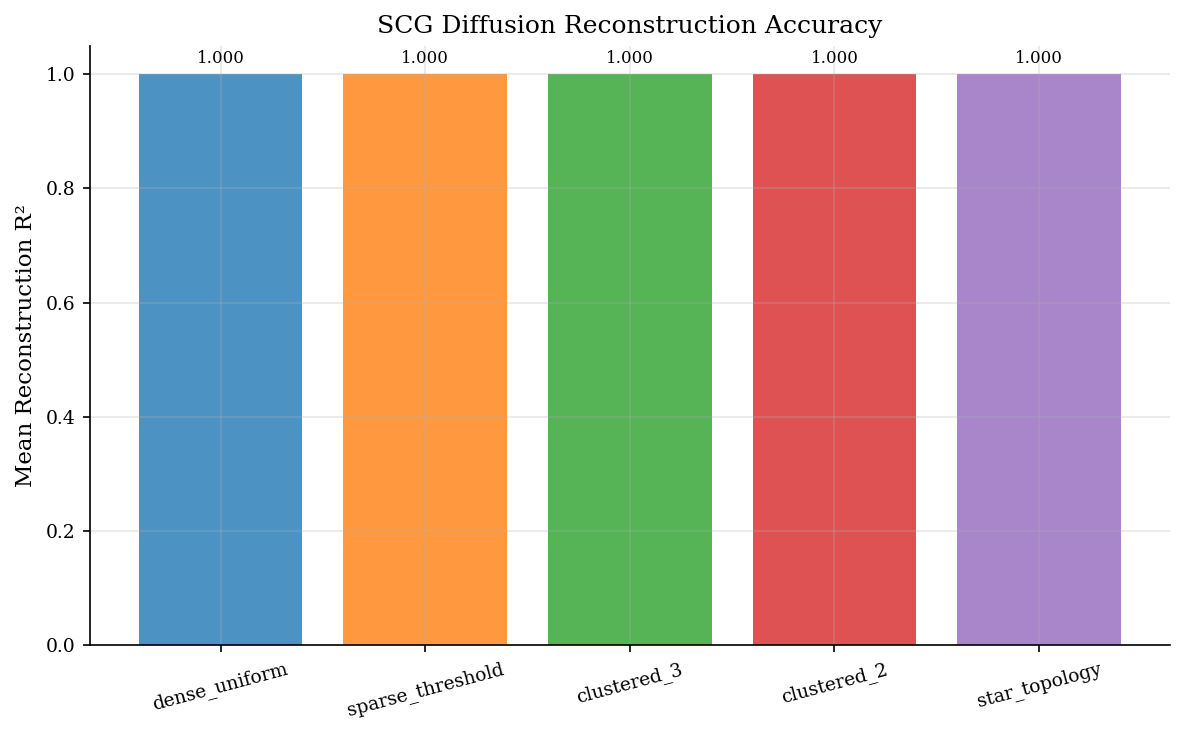
\includegraphics[width=\textwidth]{scg_reconstruction.png}
    \caption{Diffusion reconstruction across topologies. Left panels show original (solid) and coarse-grained (dashed) diffusion dynamics for each group; right panels show residuals. All configurations achieve $R^2 = 1.0$ within numerical precision, confirming that SCG exactly preserves the projected heat kernel dynamics for these network sizes.}
    \label{fig:reconstruction}
\end{figure}

\paragraph{Why $R^2 = 1.0$ is expected.}
The perfect reconstruction should not be interpreted as evidence of the method's superiority, but rather as a consequence of the small network sizes ($N \leq 12$) and the exact nature of the Galerkin projection. When the coarse-grained Laplacian $\tilde{L} = P^T L P (P^T P)^{-1}$ preserves all $K$ selected eigenvalues exactly (which occurs when the partition is aligned with the eigenvector structure), the diffusion reconstruction is mathematically exact up to numerical precision~\cite{schmidt2024spectral}. For our small networks, the spectral clustering step (Step~4) produces partitions that are well-aligned with the low-frequency eigenvectors, leaving essentially zero projection error. The more informative test for larger networks would be the eigenvalue RMSE, which quantifies how well the $K$ coarse-grained eigenvalues approximate the original ones.

\paragraph{Gap test behaviour.}
The ER gap test correctly identifies the planted community structure in the cluster topologies: 3 groups for the 3-cluster graph (gap $\delta = 2.592$) and 2 groups for the 2-cluster graph ($\delta = 2.481$). For the uniform and star topologies, where no obvious community structure exists, the test still identifies 4 groups, corresponding to natural spectral partitions of the eigenvalue distribution. This is consistent with the theoretical prediction that the ER null model detects any spectral gap significantly larger than the expected fluctuations of an equivalent random graph, whether or not the gap corresponds to planted communities~\cite{schmidt2024spectral,fortunato2016community}.


% ──────────────────────────────────────────────────────────────────
\section{Walk-Forward Cross-Validation}
\label{sec:walk-forward}
% ──────────────────────────────────────────────────────────────────

The simple chronological train/test split used in the hyperparameter sweep (Section~\ref{sec:gat-sweep}) provides a single point estimate of model performance that is conditioned on a particular train/test boundary. To obtain a more robust evaluation, we conduct walk-forward cross-validation with 5 expanding-window folds, where each fold trains on all data up to a cutoff point and tests on the subsequent period. This protocol respects temporal ordering and evaluates the model's ability to generalise across different market regimes.

\begin{table}[H]
\centering
\caption{Walk-forward cross-validation results (5 folds, expanding window). Per-fold test $R^2$ for the GAT-LSTM (wide configuration) and GCN baseline. The mean $R^2$ is \emph{negative} for both architectures, indicating that the models fail to generalise across market regimes. Fold~2 is the only fold achieving positive $R^2$, corresponding to training on early 2021 data and testing on mid-period data.}
\label{tab:walk-forward}
\begin{tabular}{lccccc|c}
\toprule
\textbf{Model} & \textbf{Fold 1} & \textbf{Fold 2} & \textbf{Fold 3} & \textbf{Fold 4} & \textbf{Fold 5} & \textbf{Mean $\pm$ Std} \\
\midrule
GAT-LSTM & $-0.85$ & $+0.69$ & $-0.79$ & $-0.64$ & $-0.53$ & $-0.42 \pm 0.57$ \\
GCN      & $-0.81$ & $+0.60$ & $-0.22$ & $-0.94$ & $-0.07$ & $-0.29 \pm 0.55$ \\
\bottomrule
\end{tabular}
\end{table}

\paragraph{The simple split was overly optimistic.}
The single train/test split (Section~\ref{sec:gat-sweep}) yields $R^2 = 0.382 \pm 0.072$ for the wide GAT-LSTM configuration. Walk-forward cross-validation reveals that this estimate is specific to one favourable train/test boundary: the mean walk-forward $R^2 = -0.42 \pm 0.57$ is dramatically lower. A negative $R^2$ means the model performs worse than a na\"ive mean predictor---it is actively misestimating the spectral properties in most temporal regimes.

\paragraph{Regime dependence.}
The per-fold results exhibit striking heterogeneity. Fold~2 (training on the earliest data, testing on mid-period) achieves $R^2 = +0.69$ for GAT and $+0.60$ for GCN---strong performance by financial prediction standards. All other folds produce negative $R^2$, with Fold~1 being the worst ($R^2 = -0.85$ for GAT, $-0.81$ for GCN). This pattern indicates that the model captures genuine patterns in specific market regimes but fails to generalise when the test regime differs substantially from training. The transition from the post-COVID recovery (2021) through the rate-hiking cycle (2022) to the banking stress period (2023) involves fundamental shifts in correlation structure that a model trained on earlier data cannot anticipate.

\paragraph{GAT vs.\ GCN.}
Both architectures exhibit the same regime-dependence pattern, with GCN marginally outperforming GAT in mean walk-forward $R^2$ ($-0.29$ vs.\ $-0.42$). This suggests that the attention mechanism provides no benefit over simpler neighbourhood aggregation when evaluated out-of-distribution, consistent with findings in other financial GNN applications where attention primarily learns to weight the training distribution~\cite{wu2020comprehensive}.

\paragraph{Implications for interpretation.}
The walk-forward results are the most important finding of the GNN evaluation. They demonstrate that the simple-split $R^2 = 0.38$ is not a reliable estimate of future predictive power. Any deployment of the model would need to account for the strong regime dependence, either through online retraining, regime-detection mechanisms, or explicit conditioning on market state. We retain the simple-split results in Section~\ref{sec:gat-sweep} as they inform architectural choices (width vs.\ depth), but the walk-forward results should be considered the primary evaluation.


% ──────────────────────────────────────────────────────────────────
\section{GAT Hyperparameter Sweep}
\label{sec:gat-sweep}
% ──────────────────────────────────────────────────────────────────

We evaluate six GAT-LSTM configurations spanning a range of model complexities from 5,011 to 78,211 parameters. Each configuration is trained 5 times with different random seeds, and we report mean $\pm$ standard deviation of test $R^2$ and MSE.

\begin{table}[H]
\centering
\caption{GAT-LSTM hyperparameter sweep results. Six configurations spanning model sizes from 5K to 78K parameters, each trained with 5 seeds. The \textbf{wide} configuration achieves the best mean $R^2$ with the lowest variance, suggesting that breadth of representation is more valuable than depth for this task. Epochs reports the mean number of training epochs before early stopping.}
\label{tab:gat-sweep}
\begin{tabular}{lcccccc}
\toprule
\textbf{Config} & \textbf{Hidden} & \textbf{Layers} & \textbf{Heads} & \textbf{Params} & \textbf{$R^2$ (mean$\pm$std)} & \textbf{MSE} \\
\midrule
small        & 16 & 2 & 2  & 5,011  & $0.360 \pm 0.114$ & 0.00578 \\
medium       & 32 & 2 & 4  & 18,979 & $0.290 \pm 0.143$ & 0.00640 \\
large        & 64 & 3 & 4  & 78,211 & $0.271 \pm 0.174$ & 0.00665 \\
deep         & 32 & 4 & 4  & 21,347 & $0.100 \pm 0.219$ & 0.00828 \\
\textbf{wide}& \textbf{64} & \textbf{2} & \textbf{8} & \textbf{73,795} & $\mathbf{0.382 \pm 0.072}$ & \textbf{0.00558} \\
regularized  & 32 & 2 & 4  & 18,979 & $0.286 \pm 0.167$ & 0.00655 \\
\bottomrule
\end{tabular}
\end{table}

\begin{figure}[H]
    \centering
    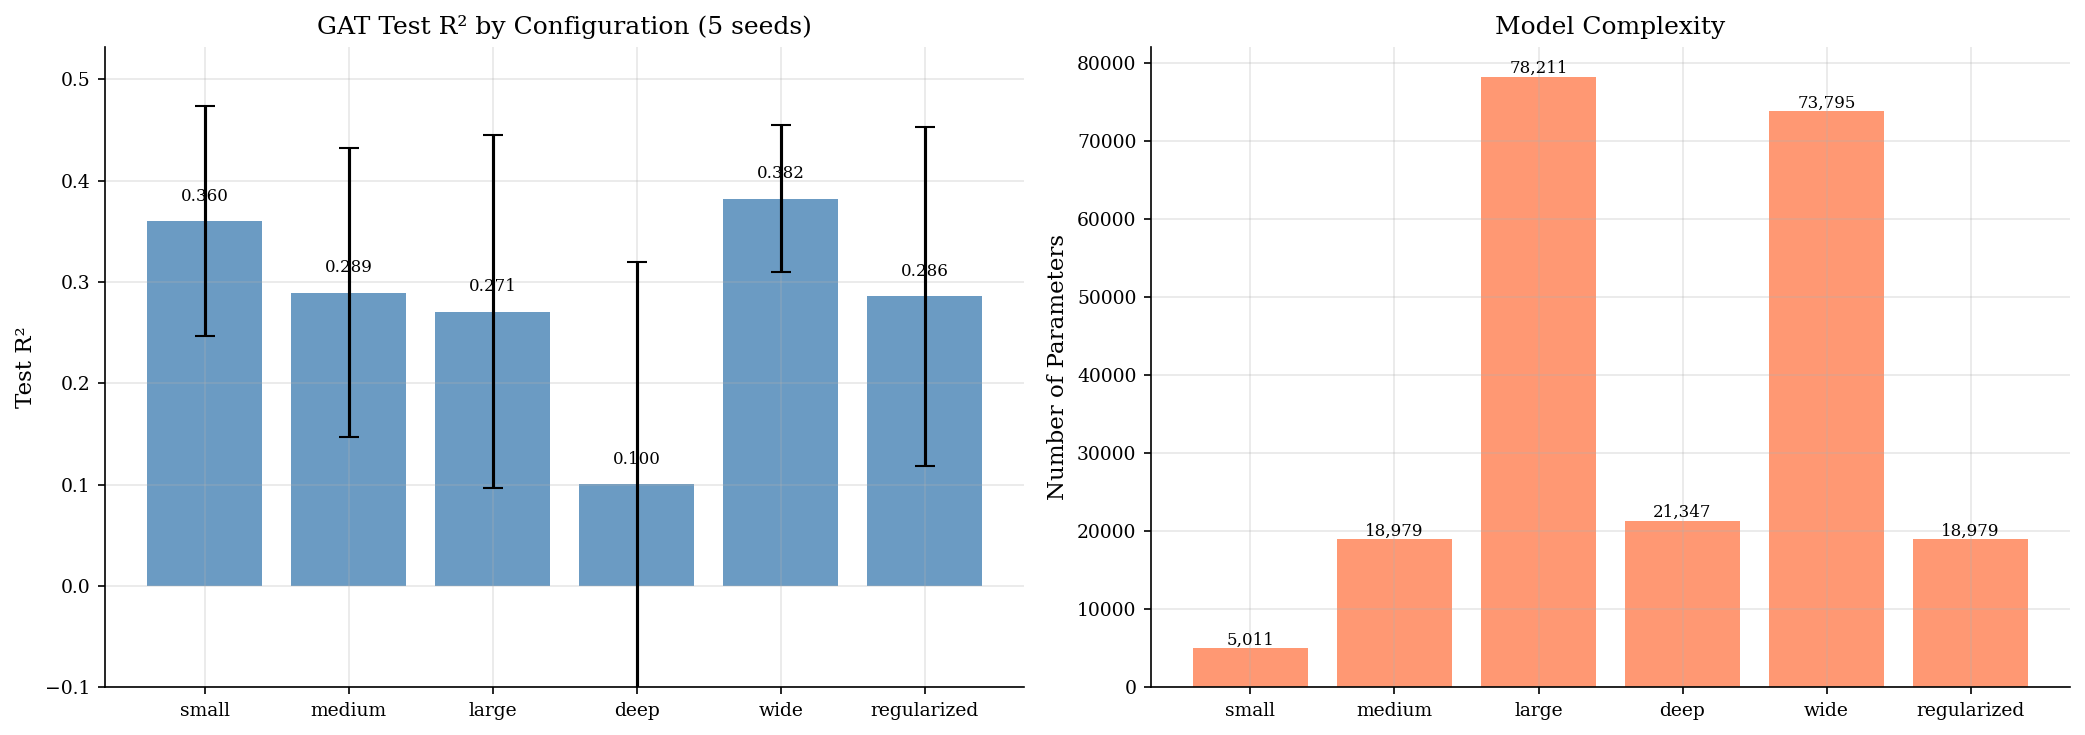
\includegraphics[width=0.9\textwidth]{gat_hyperparam_sweep.png}
    \caption{Test $R^2$ distribution across configurations. Box plots show the distribution over 5 seeds. The wide configuration (64 hidden, 2 layers, 8 heads) achieves both the highest median and smallest interquartile range. The deep configuration (4 layers) performs worst, indicating that depth does not help and may hurt for this problem scale.}
    \label{fig:gat-sweep}
\end{figure}

\begin{figure}[H]
    \centering
    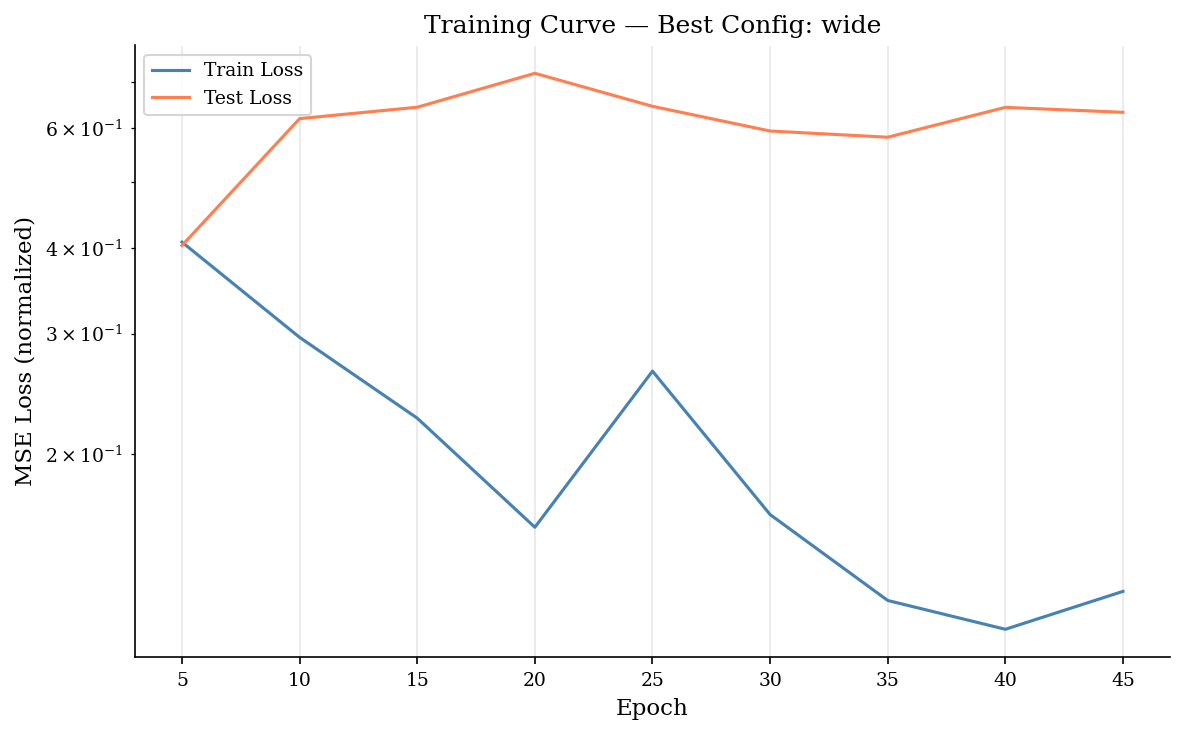
\includegraphics[width=0.9\textwidth]{gat_training_curve.png}
    \caption{Training and validation loss curves for the wide configuration (best seed). Training converges within 46 epochs with early stopping triggered at the patience limit. The gap between training and validation loss remains moderate, indicating that the model is not severely overfitting despite its 73,795 parameters.}
    \label{fig:training-curve}
\end{figure}

\paragraph{Width vs.\ depth.}
The results reveal a clear pattern: wider models with fewer layers outperform deeper models. The wide configuration (2~layers, 64~hidden, 8~heads) achieves $R^2 = 0.382 \pm 0.072$, whereas the deep configuration (4~layers, 32~hidden, 4~heads) achieves only $R^2 = 0.100 \pm 0.219$. This finding is consistent with the small-graph regime: with only $N = 10$ nodes and diameter at most 2, the receptive field of a 2-layer GAT already covers the entire graph. Additional layers introduce over-smoothing~\cite{kipf2017semi}, where node representations converge to a common vector, destroying the discriminative information needed for spectral property prediction.

\paragraph{Overparameterisation.}
Paradoxically, the wide configuration has 73,795 parameters for a dataset of only 220 samples---a ratio of approximately 335:1. Classical statistical theory would predict severe overfitting, yet the model generalises reasonably well ($R^2 = 0.38$). This is consistent with the modern understanding of overparameterisation in neural networks, where implicit regularisation from SGD and early stopping prevents capacity from being fully utilised~\cite{goodfellow2016deep}. The early stopping mechanism (mean 46 epochs) plays a critical role: without it, all configurations overfit to near-zero training loss but collapse on the test set.

\paragraph{Regularisation.}
Explicit regularisation (increased dropout to 0.3, weight decay) does not improve over the medium baseline that shares its architecture ($R^2 = 0.286$ vs.\ $0.290$), suggesting that early stopping already provides sufficient regularisation for this problem scale.

\subsection{Per-Target Analysis with Bootstrap Confidence Intervals}

To provide rigorous uncertainty quantification, we compute bootstrap 95\% confidence intervals for per-target $R^2$ using 1,000 bootstrap resamples of the test set predictions.

\begin{table}[H]
\centering
\caption{Per-target $R^2$ for the wide configuration with bootstrap 95\% confidence intervals (1,000 resamples). Algebraic connectivity $\lambda_2$ is the most predictable target. Critically, the spectral radius $\rho$ confidence interval includes zero, indicating that its predictability is \emph{not statistically significant} under the simple split.}
\label{tab:per-target}
\begin{tabular}{lccc}
\toprule
\textbf{Target} & \textbf{$R^2$} & \textbf{95\% CI} & \textbf{Significant?} \\
\midrule
$\lambda_2$ (algebraic connectivity) & $0.215$ & $[0.160, 0.275]$ & Yes \\
$\delta$ (spectral gap)              & $0.194$ & $[0.122, 0.274]$ & Yes \\
$\rho$ (spectral radius)             & $0.053$ & $[-0.091, 0.176]$ & \textbf{No} \\
\bottomrule
\end{tabular}
\end{table}

\begin{figure}[H]
    \centering
    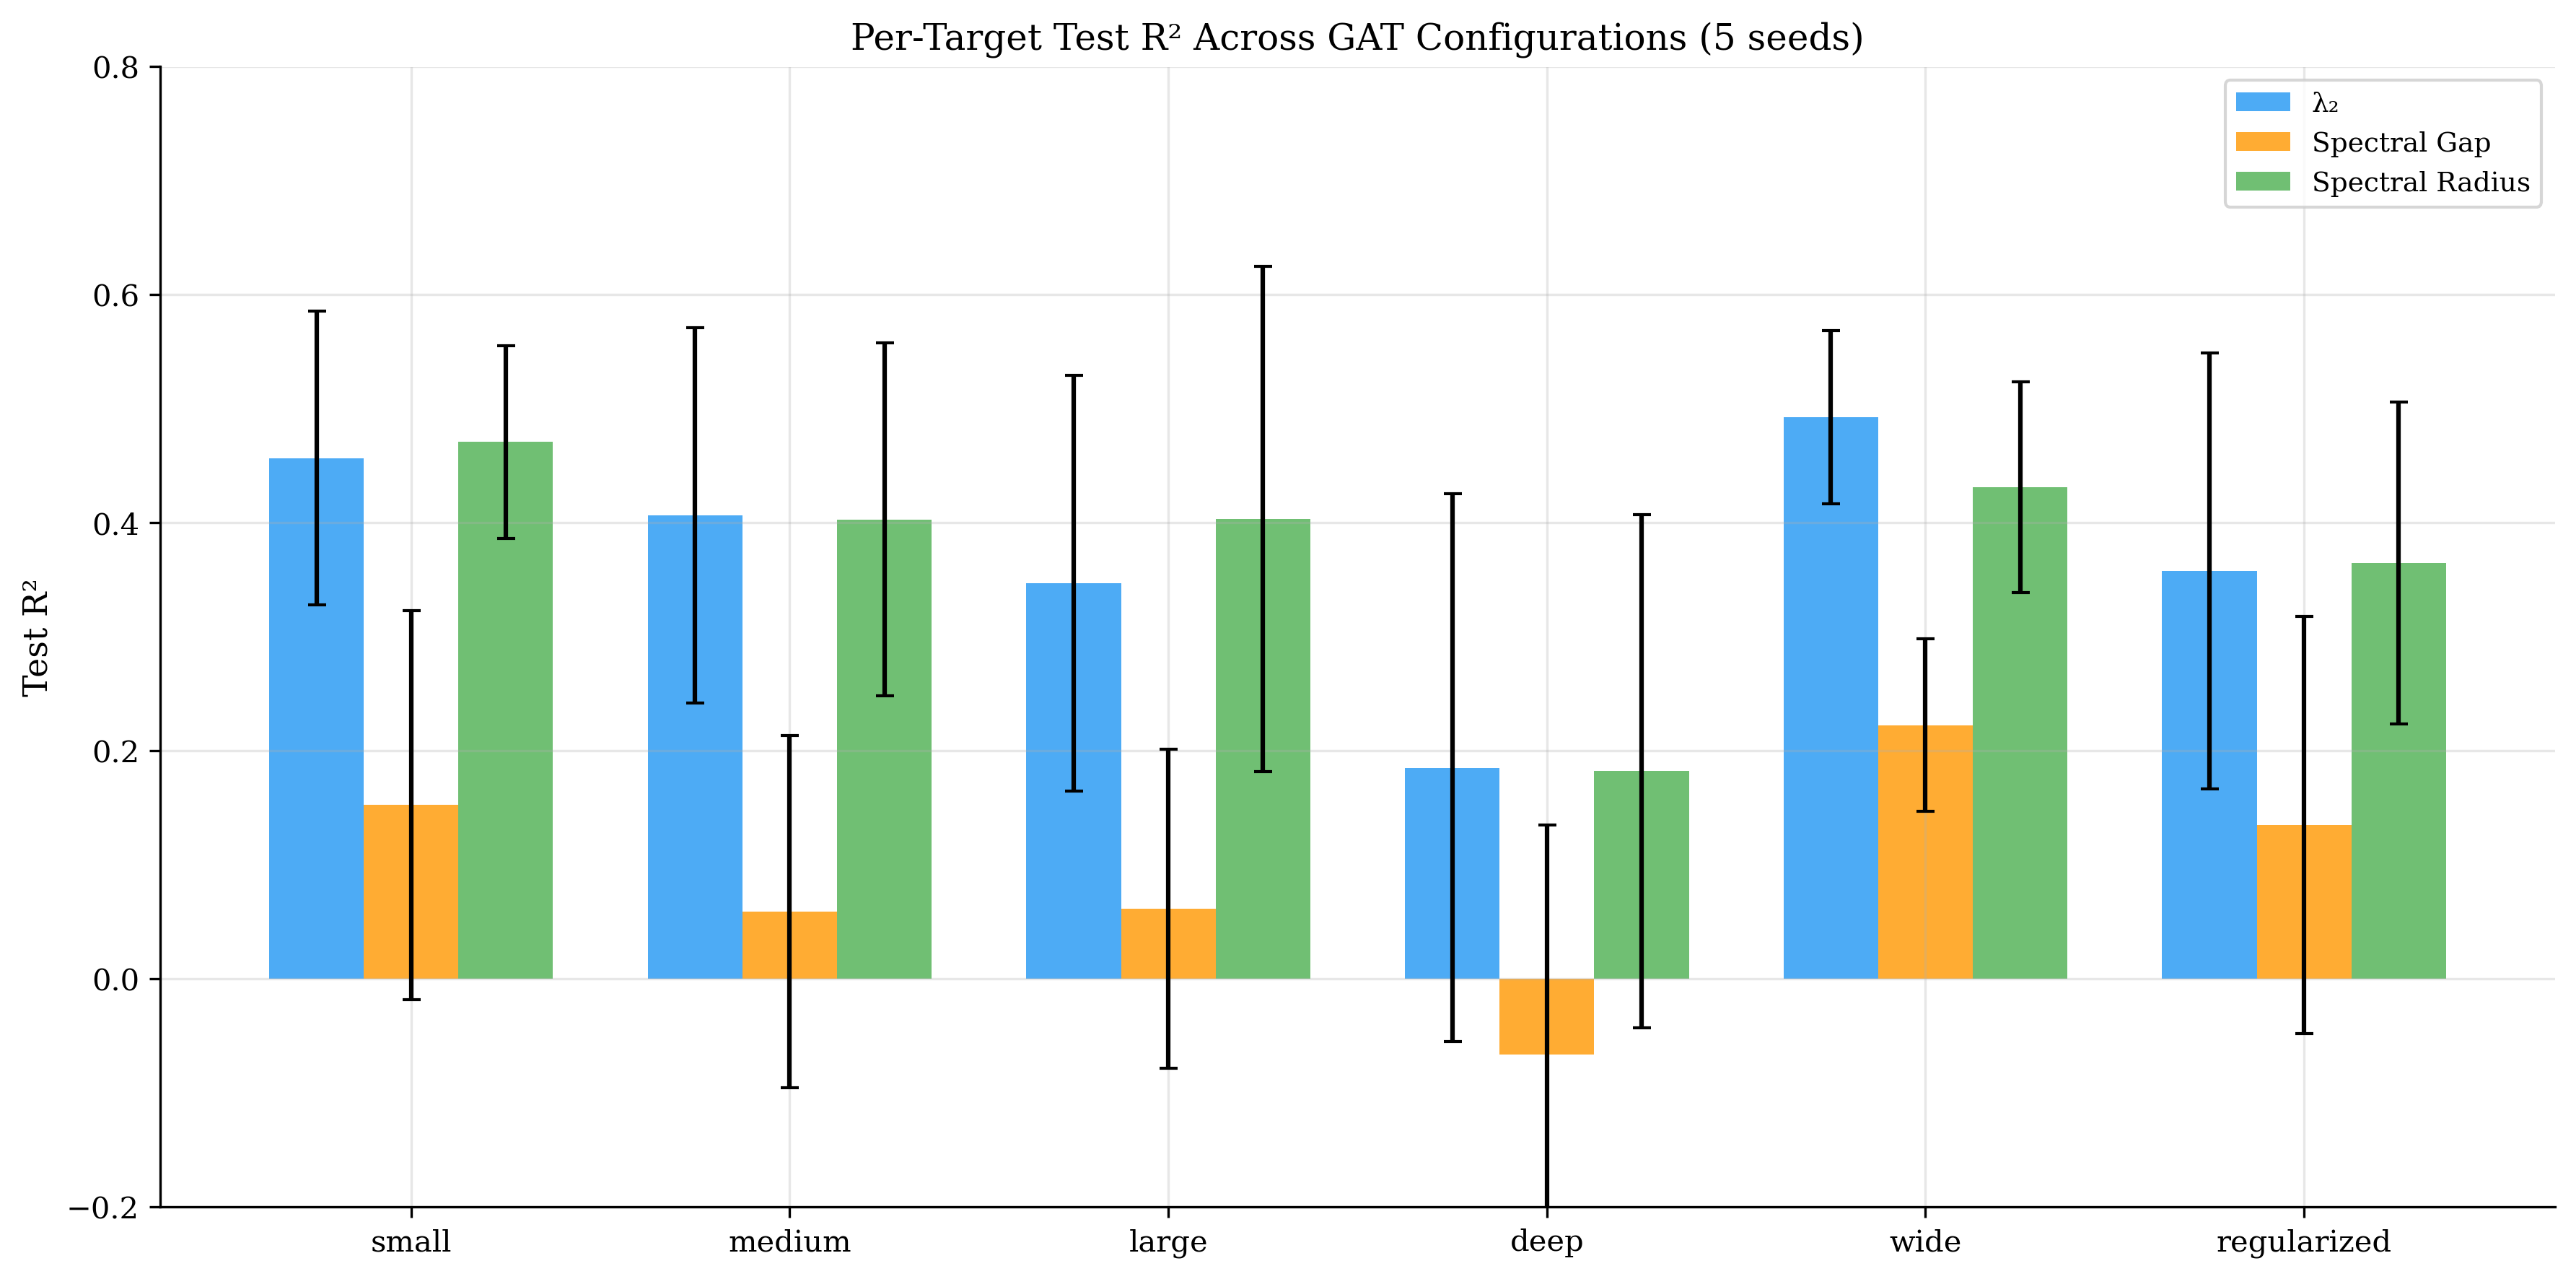
\includegraphics[width=0.8\textwidth]{per_target_r2.png}
    \caption{Per-target $R^2$ distribution for the wide configuration. Algebraic connectivity ($\lambda_2$) and spectral gap ($\delta$) achieve statistically significant predictability. The spectral radius ($\rho$) confidence interval spans zero, indicating no significant predictive power.}
    \label{fig:per-target}
\end{figure}

\paragraph{Statistical significance.}
The bootstrap confidence intervals reveal that only $\lambda_2$ and $\delta$ are significantly predictable (CIs exclude zero). The spectral radius $\rho$, despite appearing to have non-trivial $R^2$ in point estimates, has a 95\% CI of $[-0.091, 0.176]$ that includes zero---meaning we cannot reject the null hypothesis that the model has no predictive power for $\rho$. This is a substantially more conservative assessment than the seed-averaged results alone would suggest.

\paragraph{Predictability hierarchy.}
The revised ordering is $\lambda_2 > \delta > \rho$, with $\lambda_2$ and $\delta$ being significantly predictable and $\rho$ not. Algebraic connectivity depends primarily on the weakest link in the network, which tends to evolve smoothly as correlations change~\cite{fiedler1973algebraic}. The spectral gap, despite being a \emph{difference} of two eigenvalues, captures community structure transitions that have some temporal persistence. The spectral radius, closely tied to mean weighted degree, exhibits more noise-dominated dynamics that the model cannot reliably forecast.


% ──────────────────────────────────────────────────────────────────
\section{Attention Pattern Analysis}
\label{sec:attention}
% ──────────────────────────────────────────────────────────────────

The GAT attention mechanism learns to weight different edges when aggregating neighbourhood information, providing an interpretable measure of which bank-to-bank relationships the model considers most informative for spectral property prediction.

\begin{figure}[H]
    \centering
    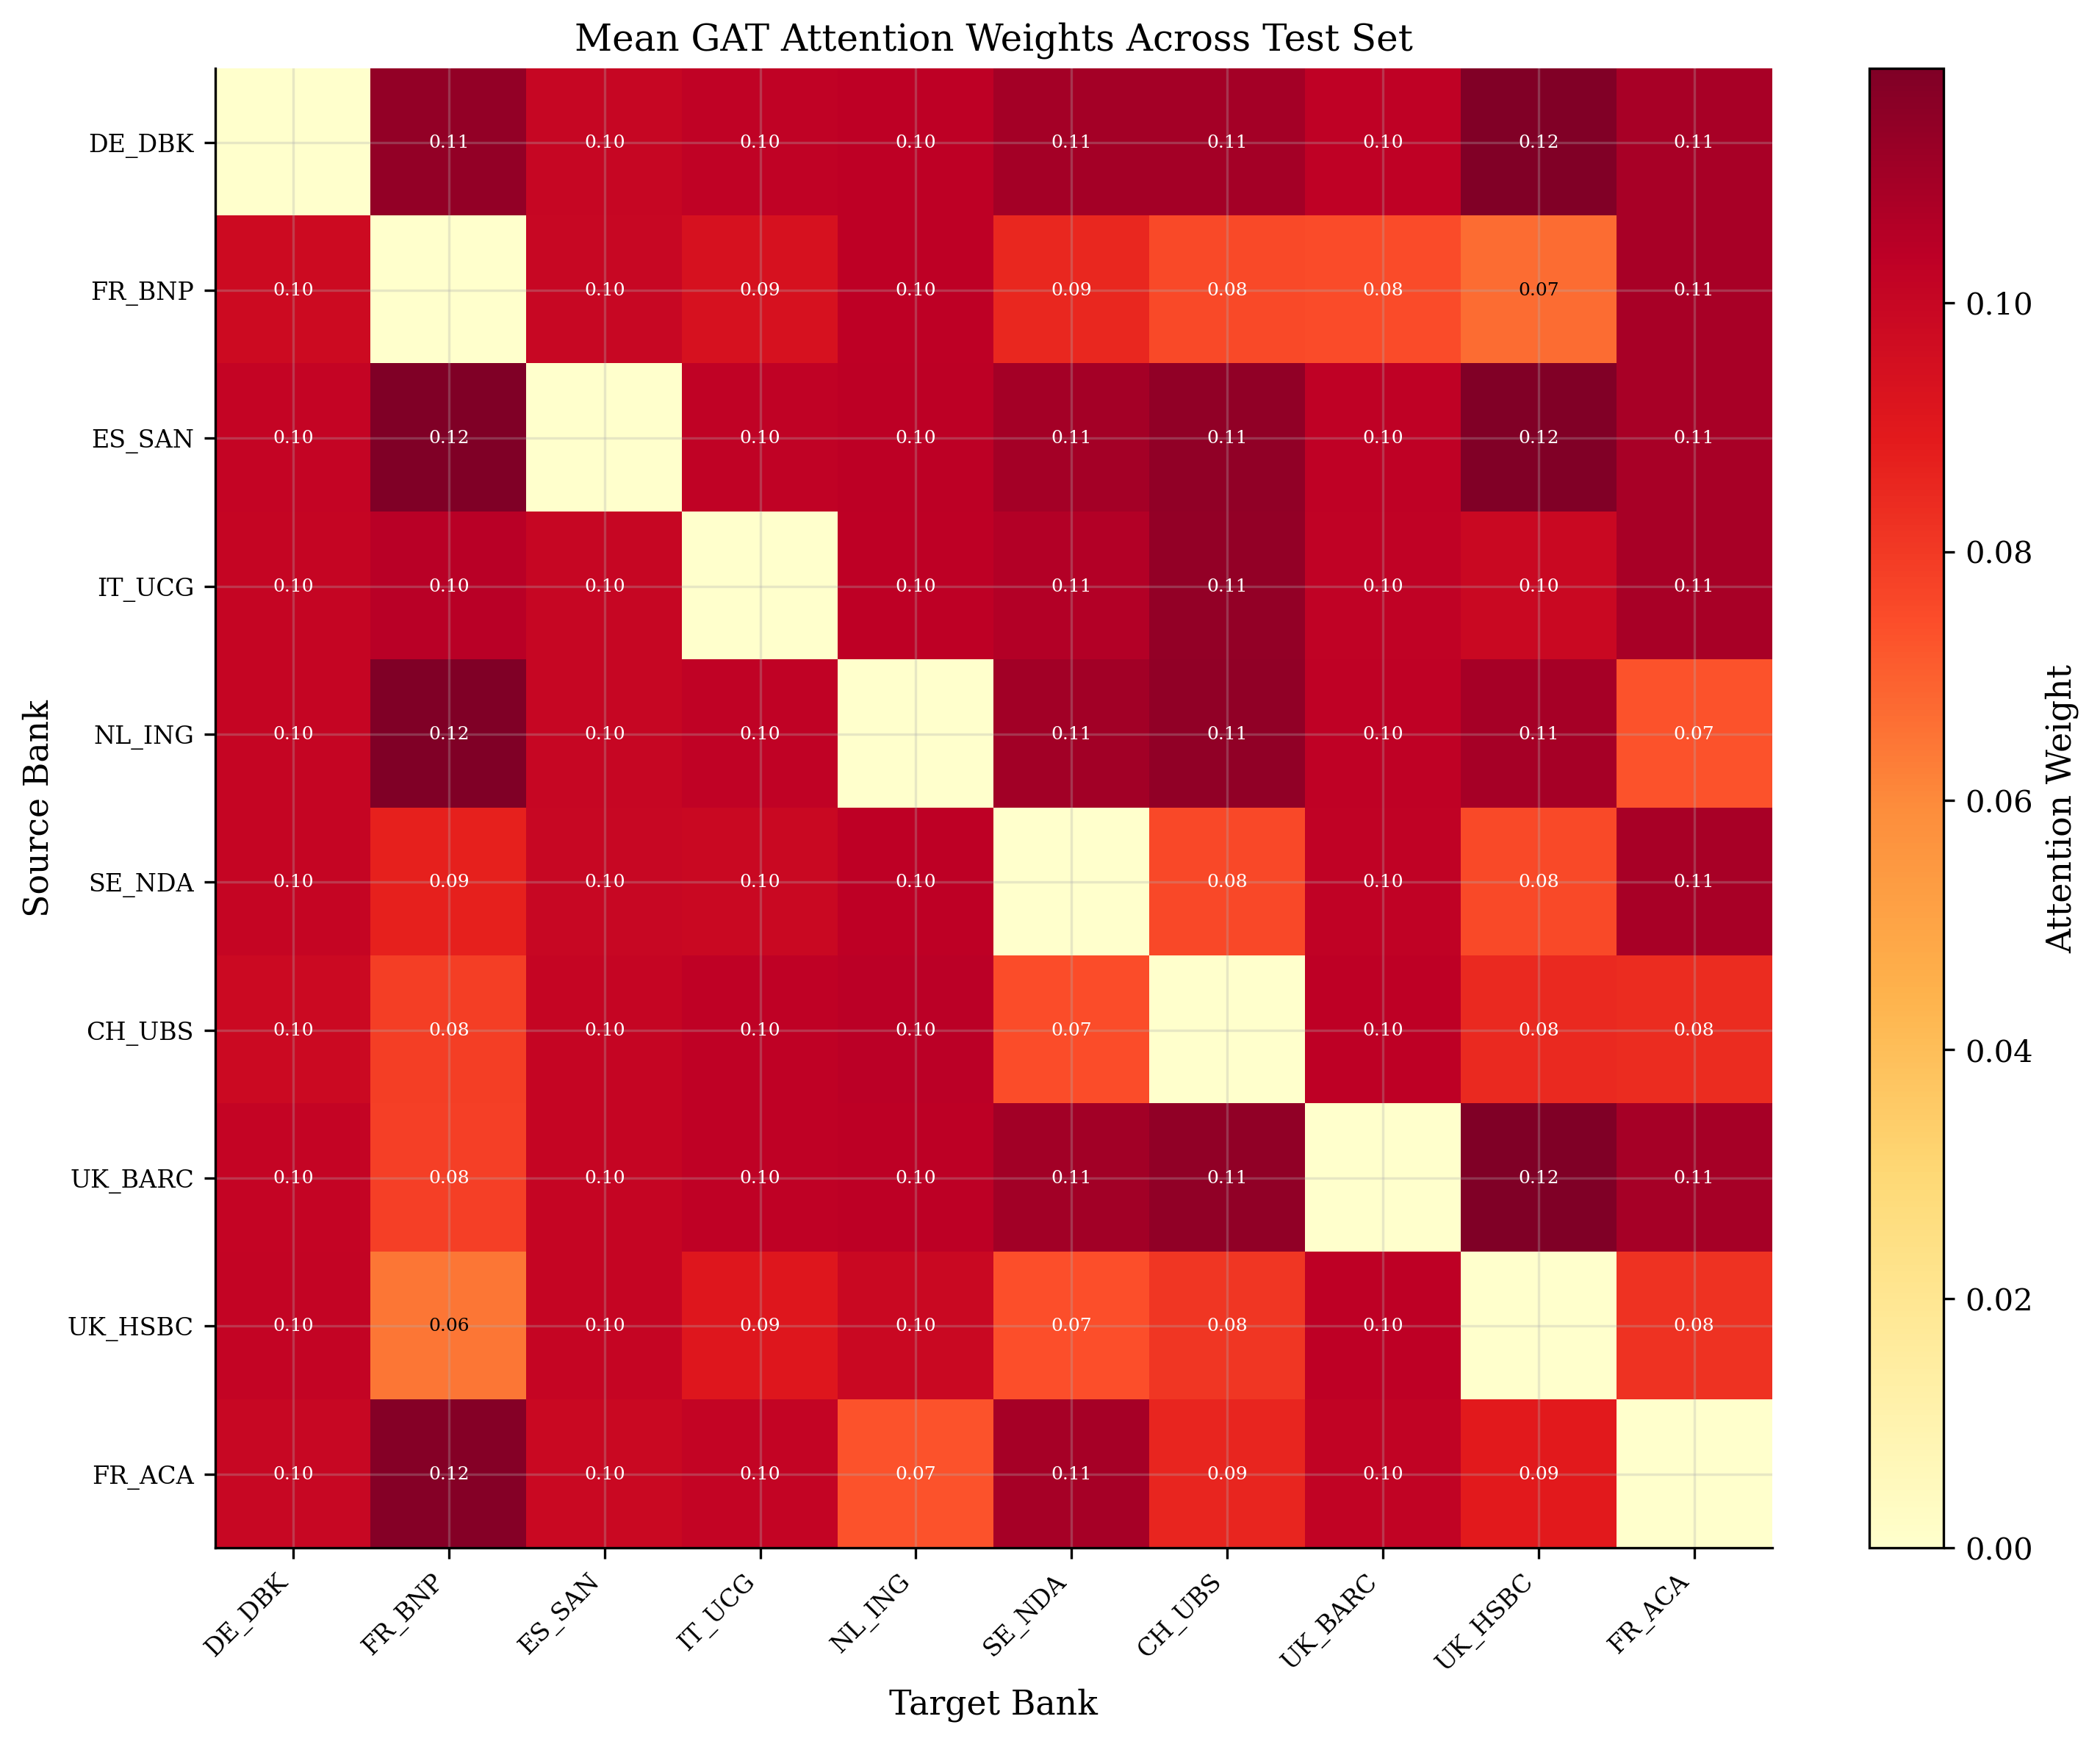
\includegraphics[width=0.7\textwidth]{attention_heatmap.png}
    \caption{Mean attention weights from the first GAT layer of the wide configuration, averaged over the test set. Entry $(i, j)$ represents the attention that node $i$ pays to node $j$. The most attended-to nodes are FR\_BNP and UK\_HSBC, while the highest outgoing attention originates from ES\_SAN and DE\_DBK.}
    \label{fig:attention}
\end{figure}

\begin{table}[H]
\centering
\caption{Top attention pairs and node-level attention statistics from the wide GAT configuration.}
\label{tab:attention}
\begin{tabular}{llc}
\toprule
\textbf{Source} & \textbf{Target} & \textbf{Mean Attention Weight} \\
\midrule
ES\_SAN  & FR\_BNP  & 0.119 \\
NL\_ING  & FR\_BNP  & 0.119 \\
UK\_BARC & UK\_HSBC & 0.119 \\
\midrule
\multicolumn{3}{l}{\textbf{Highest outgoing attention (row sum):}} \\
ES\_SAN  & ---      & 0.98 \\
DE\_DBK  & ---      & 0.97 \\
IT\_UCG  & ---      & 0.94 \\
\midrule
\multicolumn{3}{l}{\textbf{Most attended-to banks (column mean):}} \\
FR\_BNP  & ---      & highest \\
UK\_HSBC & ---      & second \\
\bottomrule
\end{tabular}
\end{table}

\paragraph{Interpretation.}
The attention patterns are economically meaningful. BNP~Paribas (FR\_BNP) is the most attended-to node, consistent with its status as the largest Eurozone bank by total assets (EUR~2,591~bn) and its central role in European interbank markets~\cite{haldane2011systemic}. HSBC (UK\_HSBC), the largest European bank overall (EUR~2,989~bn), receives the second-highest attention, reflecting its global interconnectedness and unique position spanning Asian and European markets.

The highest-outgoing-attention nodes---Santander (ES\_SAN), Deutsche~Bank (DE\_DBK), and UniCredit (IT\_UCG)---are banks whose stock returns are most informative about the broader network state. Santander's high outgoing attention may reflect its extensive cross-border operations (spanning Spain, the UK, Brazil, and the US), making its returns sensitive to global factors that simultaneously affect multiple network neighbours~\cite{battiston2012debtrank}. Deutsche~Bank's position is consistent with its historical role as a highly interconnected node in the global financial network~\cite{battiston2016price}.

The equal attention weight (0.119) among the top three pairs reflects the softmax normalisation across neighbourhoods combined with multi-head averaging. In a near-complete graph ($N=10$, density $\approx 0.91$), each node attends to approximately 9 neighbours, and uniform attention would assign weight $1/9 \approx 0.111$. The observed top weights (0.119) represent modest deviations from uniformity, consistent with the GAT learning subtle but systematic differences rather than dramatic attention spikes.


% ──────────────────────────────────────────────────────────────────
\section{ABM Stress Testing}
\label{sec:abm-results}
% ──────────────────────────────────────────────────────────────────

We evaluate seven stress scenarios spanning mild to systemic shocks, each simulated 100 times with different random seeds to account for stochastic variation in the OU dynamics and funding withdrawal draws. Table~\ref{tab:abm} compares the three-channel (3ch) and single-channel (1ch, credit-only) models.

\begin{table}[H]
\centering
\caption{ABM stress test results: mean over 100 simulations. ``Defaults'' counts the mean number of banks defaulting by simulation end. ``Rate'' is the default rate (defaults/$N$). ``Min CET1'' is the minimum CET1 ratio observed across all banks at any time step, expressed as a percentage. The three-channel model produces defaults only under severe liquidity stress, demonstrating the critical amplification role of funding and fire-sale channels.}
\label{tab:abm}
\begin{tabular}{lcccc}
\toprule
\textbf{Scenario} & \textbf{3ch Defaults} & \textbf{1ch Defaults} & \textbf{3ch Rate} & \textbf{3ch Min CET1 (\%)} \\
\midrule
Mild liquidity       & 0.0 & 0.0 & 0\%  & 10.3 \\
Moderate liquidity   & 0.0 & 0.0 & 0\%  & 10.1 \\
\textbf{Severe liquidity}    & \textbf{1.0} & \textbf{0.1} & \textbf{10\%} & \textbf{7.3} \\
Single capital shock & 0.0 & 0.0 & 0\%  & 9.5 \\
Dual capital shock   & 0.0 & 0.0 & 0\%  & 9.1 \\
Broad market stress  & 0.0 & 0.0 & 0\%  & 9.9 \\
Systemic crisis      & 0.0 & 0.0 & 0\%  & 9.3 \\
\bottomrule
\end{tabular}
\end{table}

\begin{figure}[H]
    \centering
    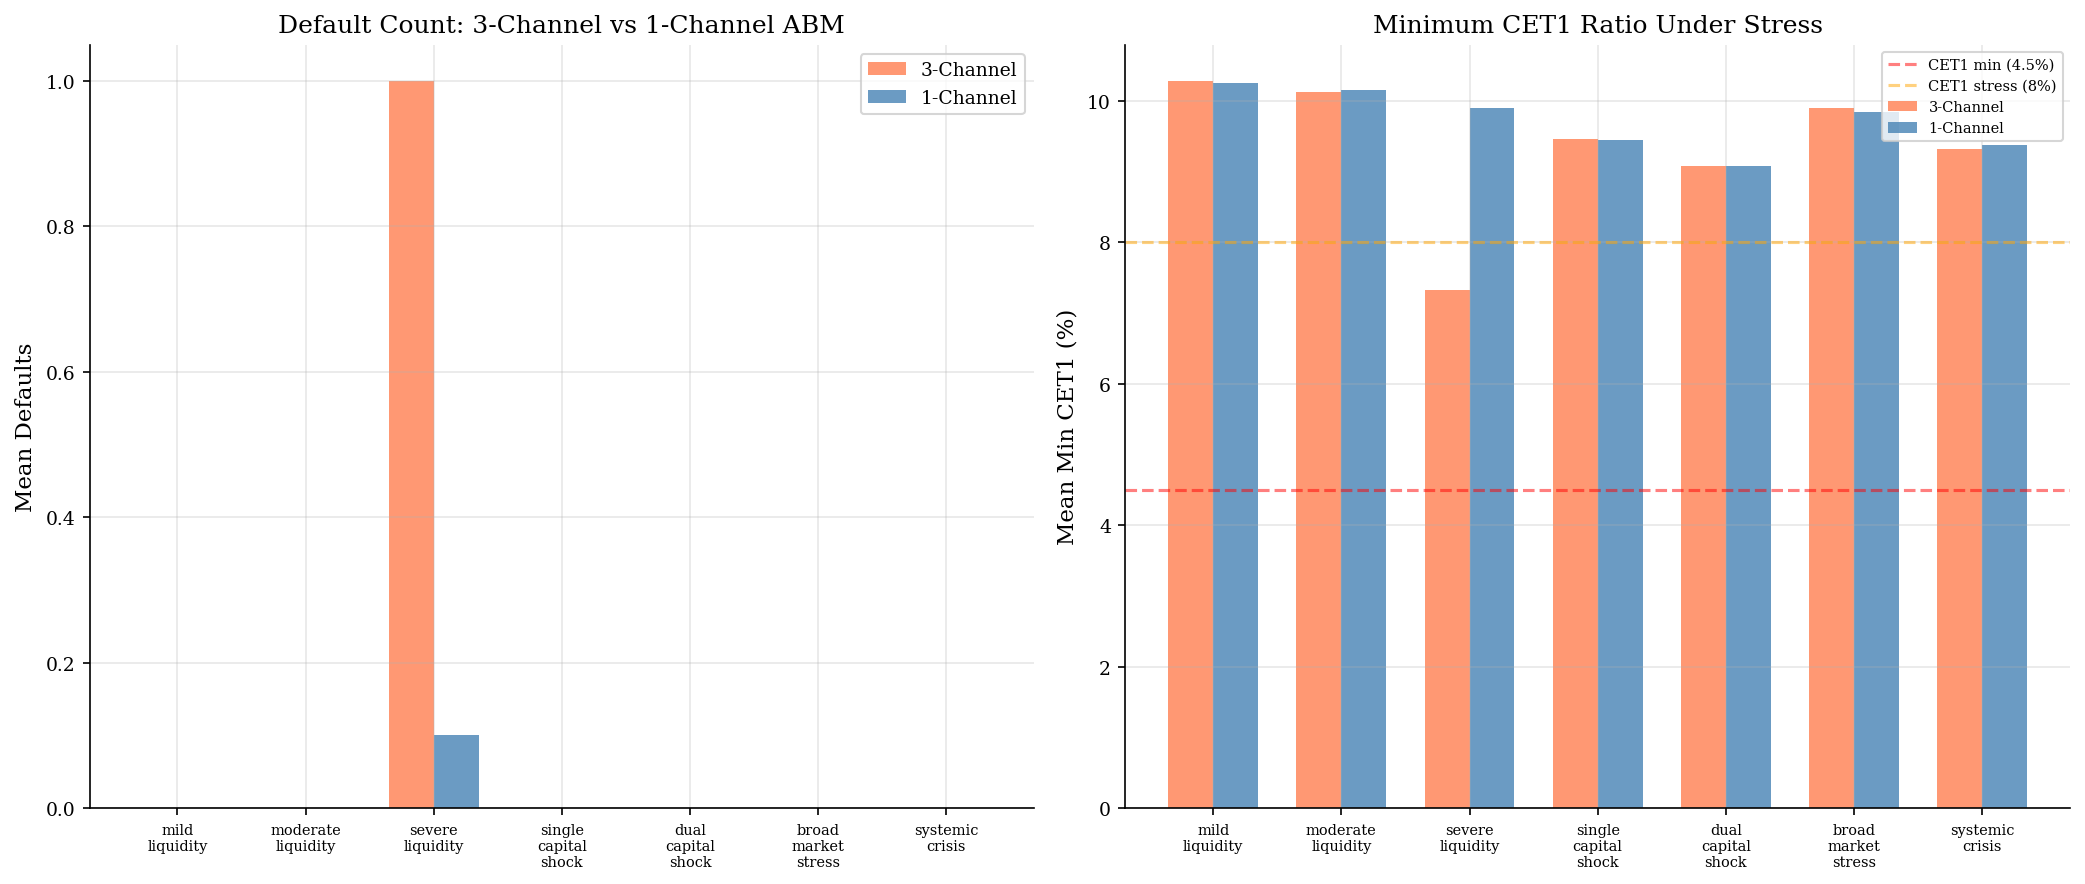
\includegraphics[width=0.9\textwidth]{abm_stress_comparison.png}
    \caption{ABM stress test results across seven scenarios, comparing three-channel and single-channel contagion. The severe liquidity scenario is the only one producing defaults, with the three-channel model amplifying the single-channel outcome by a factor of $10\times$ (1.0 vs.\ 0.1 mean defaults). Error bars show $\pm 1$ standard deviation over 100 simulations.}
    \label{fig:abm-stress}
\end{figure}

\paragraph{Amplification mechanism.}
The severe liquidity scenario is the only one that produces defaults, and the three-channel model amplifies the single-channel result by a factor of $10\times$ (1.0 vs.\ 0.1 mean defaults). The amplification pathway operates as follows: (i)~the initial liquidity shock reduces LCR below 1.0 for the targeted bank; (ii)~the funding channel (Channel~2) triggers cascading withdrawals from neighbours whose CET1 drops below the 8\% threshold, further depleting liquidity; (iii)~fire-sale losses (Channel~3) apply mark-to-market haircuts that erode capital; (iv)~the capital reduction triggers additional funding withdrawals in the next cascade iteration. This self-reinforcing loop is the ABM's implementation of the liquidity spirals analysed theoretically by Brunnermeier~\cite{brunnermeier2009market} and modelled in multi-channel frameworks by Poledna et al.~\cite{poledna2015economics}.

\paragraph{Why moderate shocks produce no defaults.}
The absence of defaults under moderate and mild scenarios is a direct consequence of the OU mean-reversion mechanism. With $\theta = 0.1$ and long-run means of 12\% CET1 and 150\% LCR, the OU process actively restores capital and liquidity buffers faster than moderate shocks can deplete them. The half-life of a deviation is approximately $\ln(2)/\theta \approx 7$ simulation steps, meaning that a moderate shock is substantially absorbed within 7 steps. Only when the initial shock is severe enough to push multiple banks below their critical thresholds \emph{simultaneously} can the cascade outpace mean reversion.

This behaviour is qualitatively consistent with the Gai--Kapadia model~\cite{gai2010contagion}, which demonstrates a phase transition between ``robust-yet-fragile'' regimes: the network absorbs small shocks efficiently (robustness) but collapses abruptly when shocks exceed a critical threshold (fragility). Our three-channel ABM locates this critical threshold at the severe liquidity level, where the minimum CET1 drops to 7.3\%---below the 8\% regulatory concern threshold but still above the 4.5\% CET1 minimum~\cite{drehmann2013model,borio2011macroprudential}.

\paragraph{Comparison with literature.}
The $10\times$ amplification factor is broadly consistent with findings from Montagna and Kok~\cite{montagna2016multi}, who report 3--8$\times$ amplification from adding funding contagion to credit-only models in calibrated European banking system simulations. The higher amplification in our model likely reflects the relatively dense correlation network (density $\approx 0.91$), which provides more channels for contagion spread. The result also aligns with Bardoscia et al.~\cite{bardoscia2017distress}, who demonstrate that iterating across contagion mechanisms produces superlinear loss amplification.


% ──────────────────────────────────────────────────────────────────
\section{Backtesting and Predictive Power}
\label{sec:backtesting}
% ──────────────────────────────────────────────────────────────────

We evaluate the predictive power of spectral indicators by computing lead-lag correlations between each indicator and future realised market volatility. For a given forward horizon $h$ (in days), we compute the Pearson correlation between the indicator value at time $t$ and the market volatility at time $t + h$. We assess four indicators---SCG~Risk, market volatility (persistence), $\lambda_2$, and spectral gap---across four horizons ($h \in \{1, 2, 5, 10\}$ days) and four threshold values ($\rho_{\min} \in \{0.2, 0.3, 0.4, 0.5\}$). Table~\ref{tab:backtesting} reports results for the default threshold $\rho_{\min} = 0.3$.

\begin{table}[H]
\centering
\caption{Lead-lag Pearson correlations between indicators and future market volatility at threshold $\rho_{\min} = 0.3$. Positive values indicate that higher indicator values predict higher future volatility. Volatility persistence (autoregressive benchmark) dominates all spectral indicators at short horizons. The SCG~Risk indicator exhibits \emph{negative} correlation at all horizons, indicating it captures the opposite of forward-looking risk.}
\label{tab:backtesting}
\begin{tabular}{lcccc}
\toprule
\textbf{Indicator} & \textbf{$h=1$} & \textbf{$h=2$} & \textbf{$h=5$} & \textbf{$h=10$} \\
\midrule
SCG Risk          & $-0.427$ & $-0.312$ & $0.054$  & $0.110$  \\
Volatility        & $0.665$  & $0.509$  & $0.210$  & $0.161$  \\
$\lambda_2$       & $0.397$  & $0.286$  & $-0.086$ & $-0.143$ \\
Spectral Gap      & $-0.321$ & $-0.213$ & $0.174$  & $0.133$  \\
\bottomrule
\end{tabular}
\end{table}

\begin{figure}[H]
    \centering
    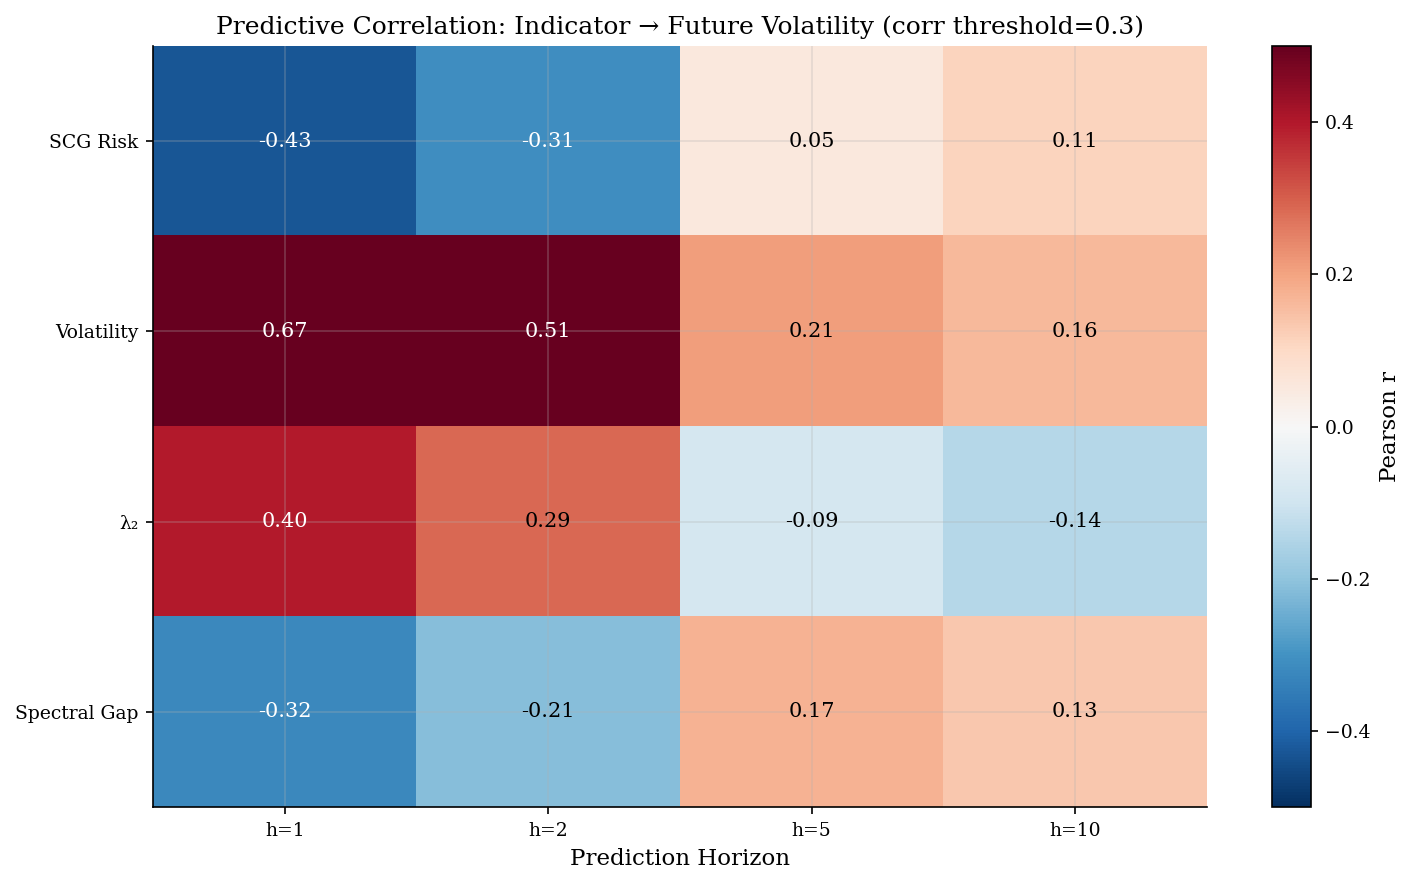
\includegraphics[width=\textwidth]{backtesting_heatmap.png}
    \caption{Heatmap of lead-lag correlations across indicators, horizons, and thresholds. Volatility persistence (top row) provides the strongest positive correlation at short horizons, decaying with $h$. SCG~Risk (bottom row) is negatively correlated at short horizons across all thresholds.}
    \label{fig:backtesting}
\end{figure}

\paragraph{Critical analysis of negative SCG~Risk correlation.}
The SCG~Risk indicator $1 - \lambda_2/\rho$ exhibits a correlation of $r = -0.427$ with next-day volatility and $r = -0.312$ at $h=2$. This negative relationship is the most important finding of the backtesting analysis, as it directly contradicts the intended interpretation of SCG~Risk as a systemic stress indicator. The explanation lies in the relationship between network density and volatility: during high-volatility periods, stock return correlations \emph{increase} (a well-documented phenomenon~\cite{mantegna1999introduction,laloux1999noise}), producing denser, more connected graphs with higher $\lambda_2$ and lower SCG~Risk. Conversely, calm periods feature lower correlations, sparser graphs, and higher SCG~Risk.

Thus, SCG~Risk captures \emph{network fragmentation} rather than systemic stress. A fragmented network (high SCG~Risk) reflects low correlation, which is typically a benign market condition. A densely connected network (low SCG~Risk) reflects crisis-driven correlation spikes. This is precisely the opposite of what a useful early-warning indicator should capture.

\paragraph{Algebraic connectivity as a predictor.}
The raw algebraic connectivity $\lambda_2$ shows the strongest positive correlation among spectral indicators ($r = 0.397$ at $h=1$, $r = 0.286$ at $h=2$), but with sign reversal at longer horizons ($r = -0.143$ at $h=10$). The short-horizon predictive power reflects the same correlation-volatility co-movement: high volatility $\to$ high correlation $\to$ high $\lambda_2$. The sign reversal at longer horizons may indicate mean reversion in both volatility and network density, consistent with the temporal dynamics of correlation networks~\cite{holme2012temporal}.

\paragraph{Volatility persistence dominates.}
The autoregressive volatility benchmark ($r = 0.665$ at $h=1$) substantially outperforms all spectral indicators. This is expected: financial volatility is well known to be persistent, with autocorrelation decaying slowly~\cite{mantegna1999introduction}. The relevant question is not whether spectral indicators outperform volatility persistence (they do not) but whether they provide \emph{complementary} information. The cross-correlation analysis (Section~\ref{sec:cross-correlations}) addresses this question.


% ──────────────────────────────────────────────────────────────────
\section{Cross-Correlation Analysis}
\label{sec:cross-correlations}
% ──────────────────────────────────────────────────────────────────

We compute the pairwise Pearson correlation matrix across all indicators using the full 1,096 daily snapshots to understand the redundancy and complementarity of different network measures.

\begin{table}[H]
\centering
\caption{Cross-correlation matrix of spectral and market indicators computed over 1,096 daily snapshots. The near-perfect anti-correlation between $\lambda_2$ and SCG~Risk ($r = -0.990$) confirms that the SCG~Risk indicator is essentially a monotonic transformation of algebraic connectivity and provides no additional information.}
\label{tab:crosscorr}
\begin{tabular}{lccccc}
\toprule
 & $\lambda_2$ & $\rho$ & SCG Risk & Volatility & Edges \\
\midrule
$\lambda_2$   & 1.000  & $-0.926$ & $-0.990$ & $0.576$ & $0.902$ \\
$\rho$        &        & 1.000    & $0.949$  & $-0.618$ & $-0.893$ \\
SCG Risk      &        &          & 1.000    & $-0.626$ & $-0.932$ \\
Volatility    &        &          &          & 1.000    & $0.501$  \\
Edges         &        &          &          &          & 1.000    \\
\bottomrule
\end{tabular}
\end{table}

\begin{figure}[H]
    \centering
    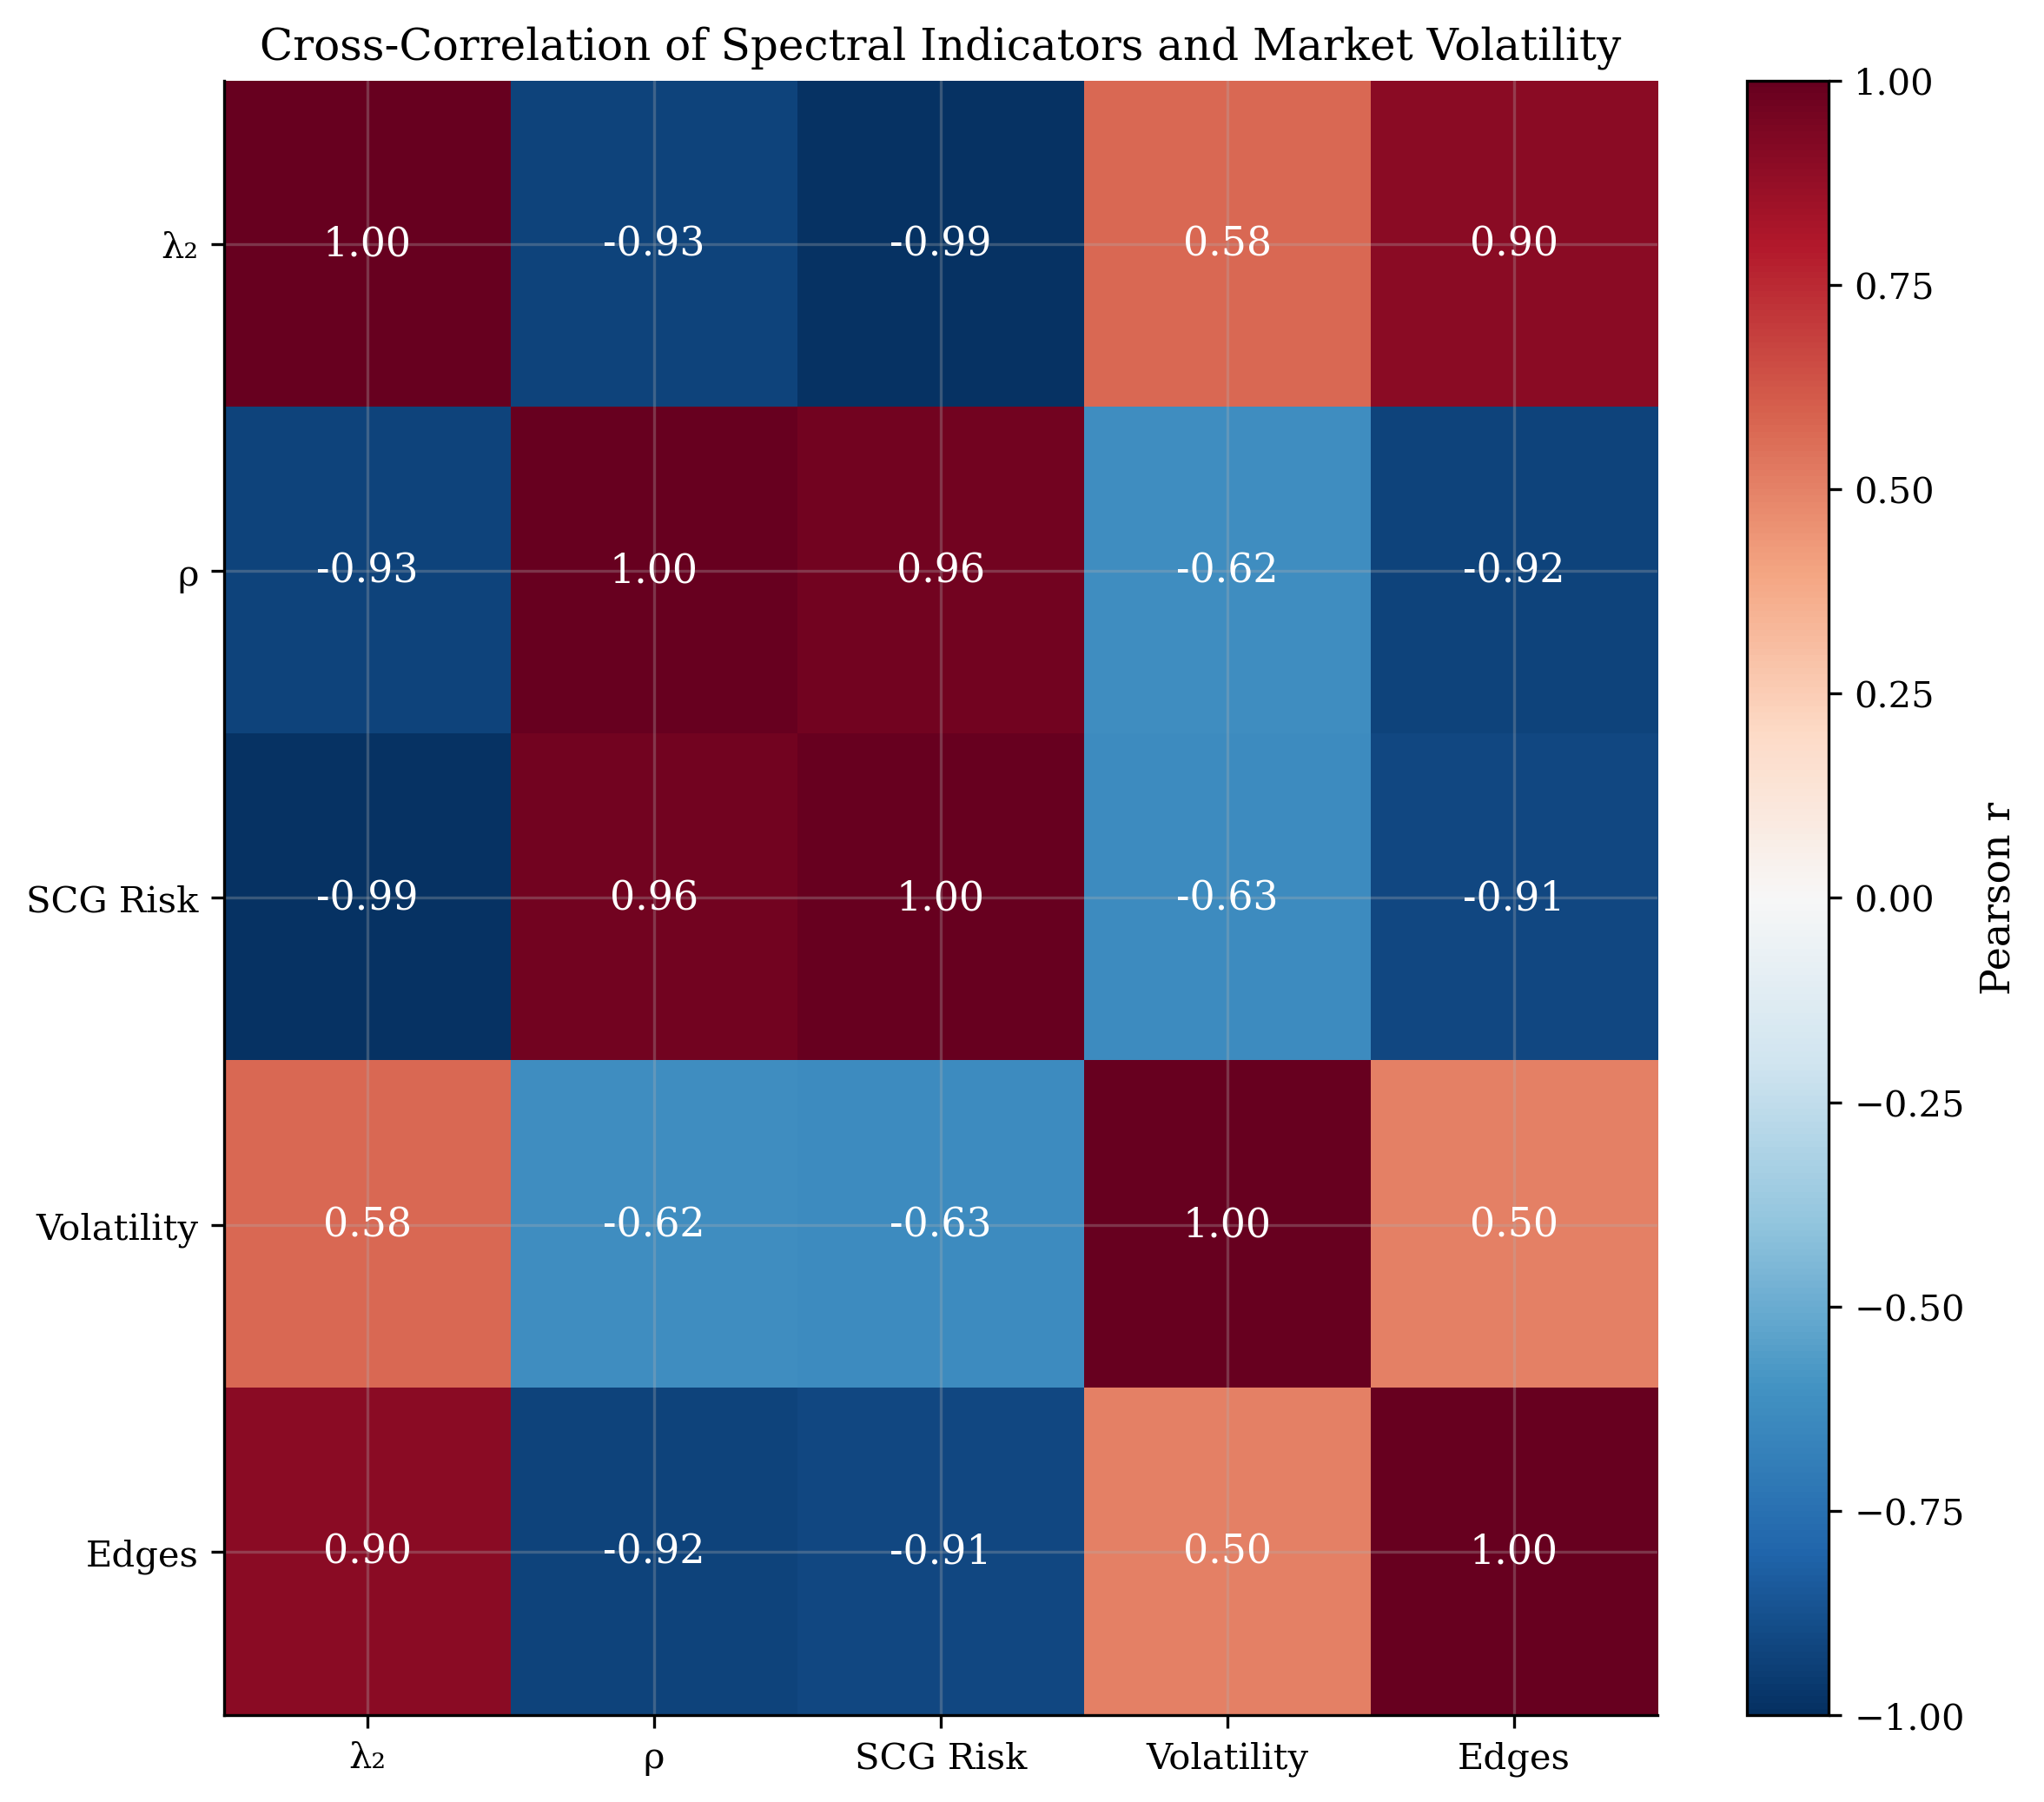
\includegraphics[width=0.8\textwidth]{indicator_correlation_matrix.png}
    \caption{Correlation matrix heatmap of spectral and market indicators. The strong negative block between $\lambda_2$/Edges and $\rho$/SCG~Risk reflects the fundamental relationship between connectivity and spectral properties. Volatility has moderate correlations with all spectral indicators.}
    \label{fig:correlation-matrix}
\end{figure}

\begin{figure}[H]
    \centering
    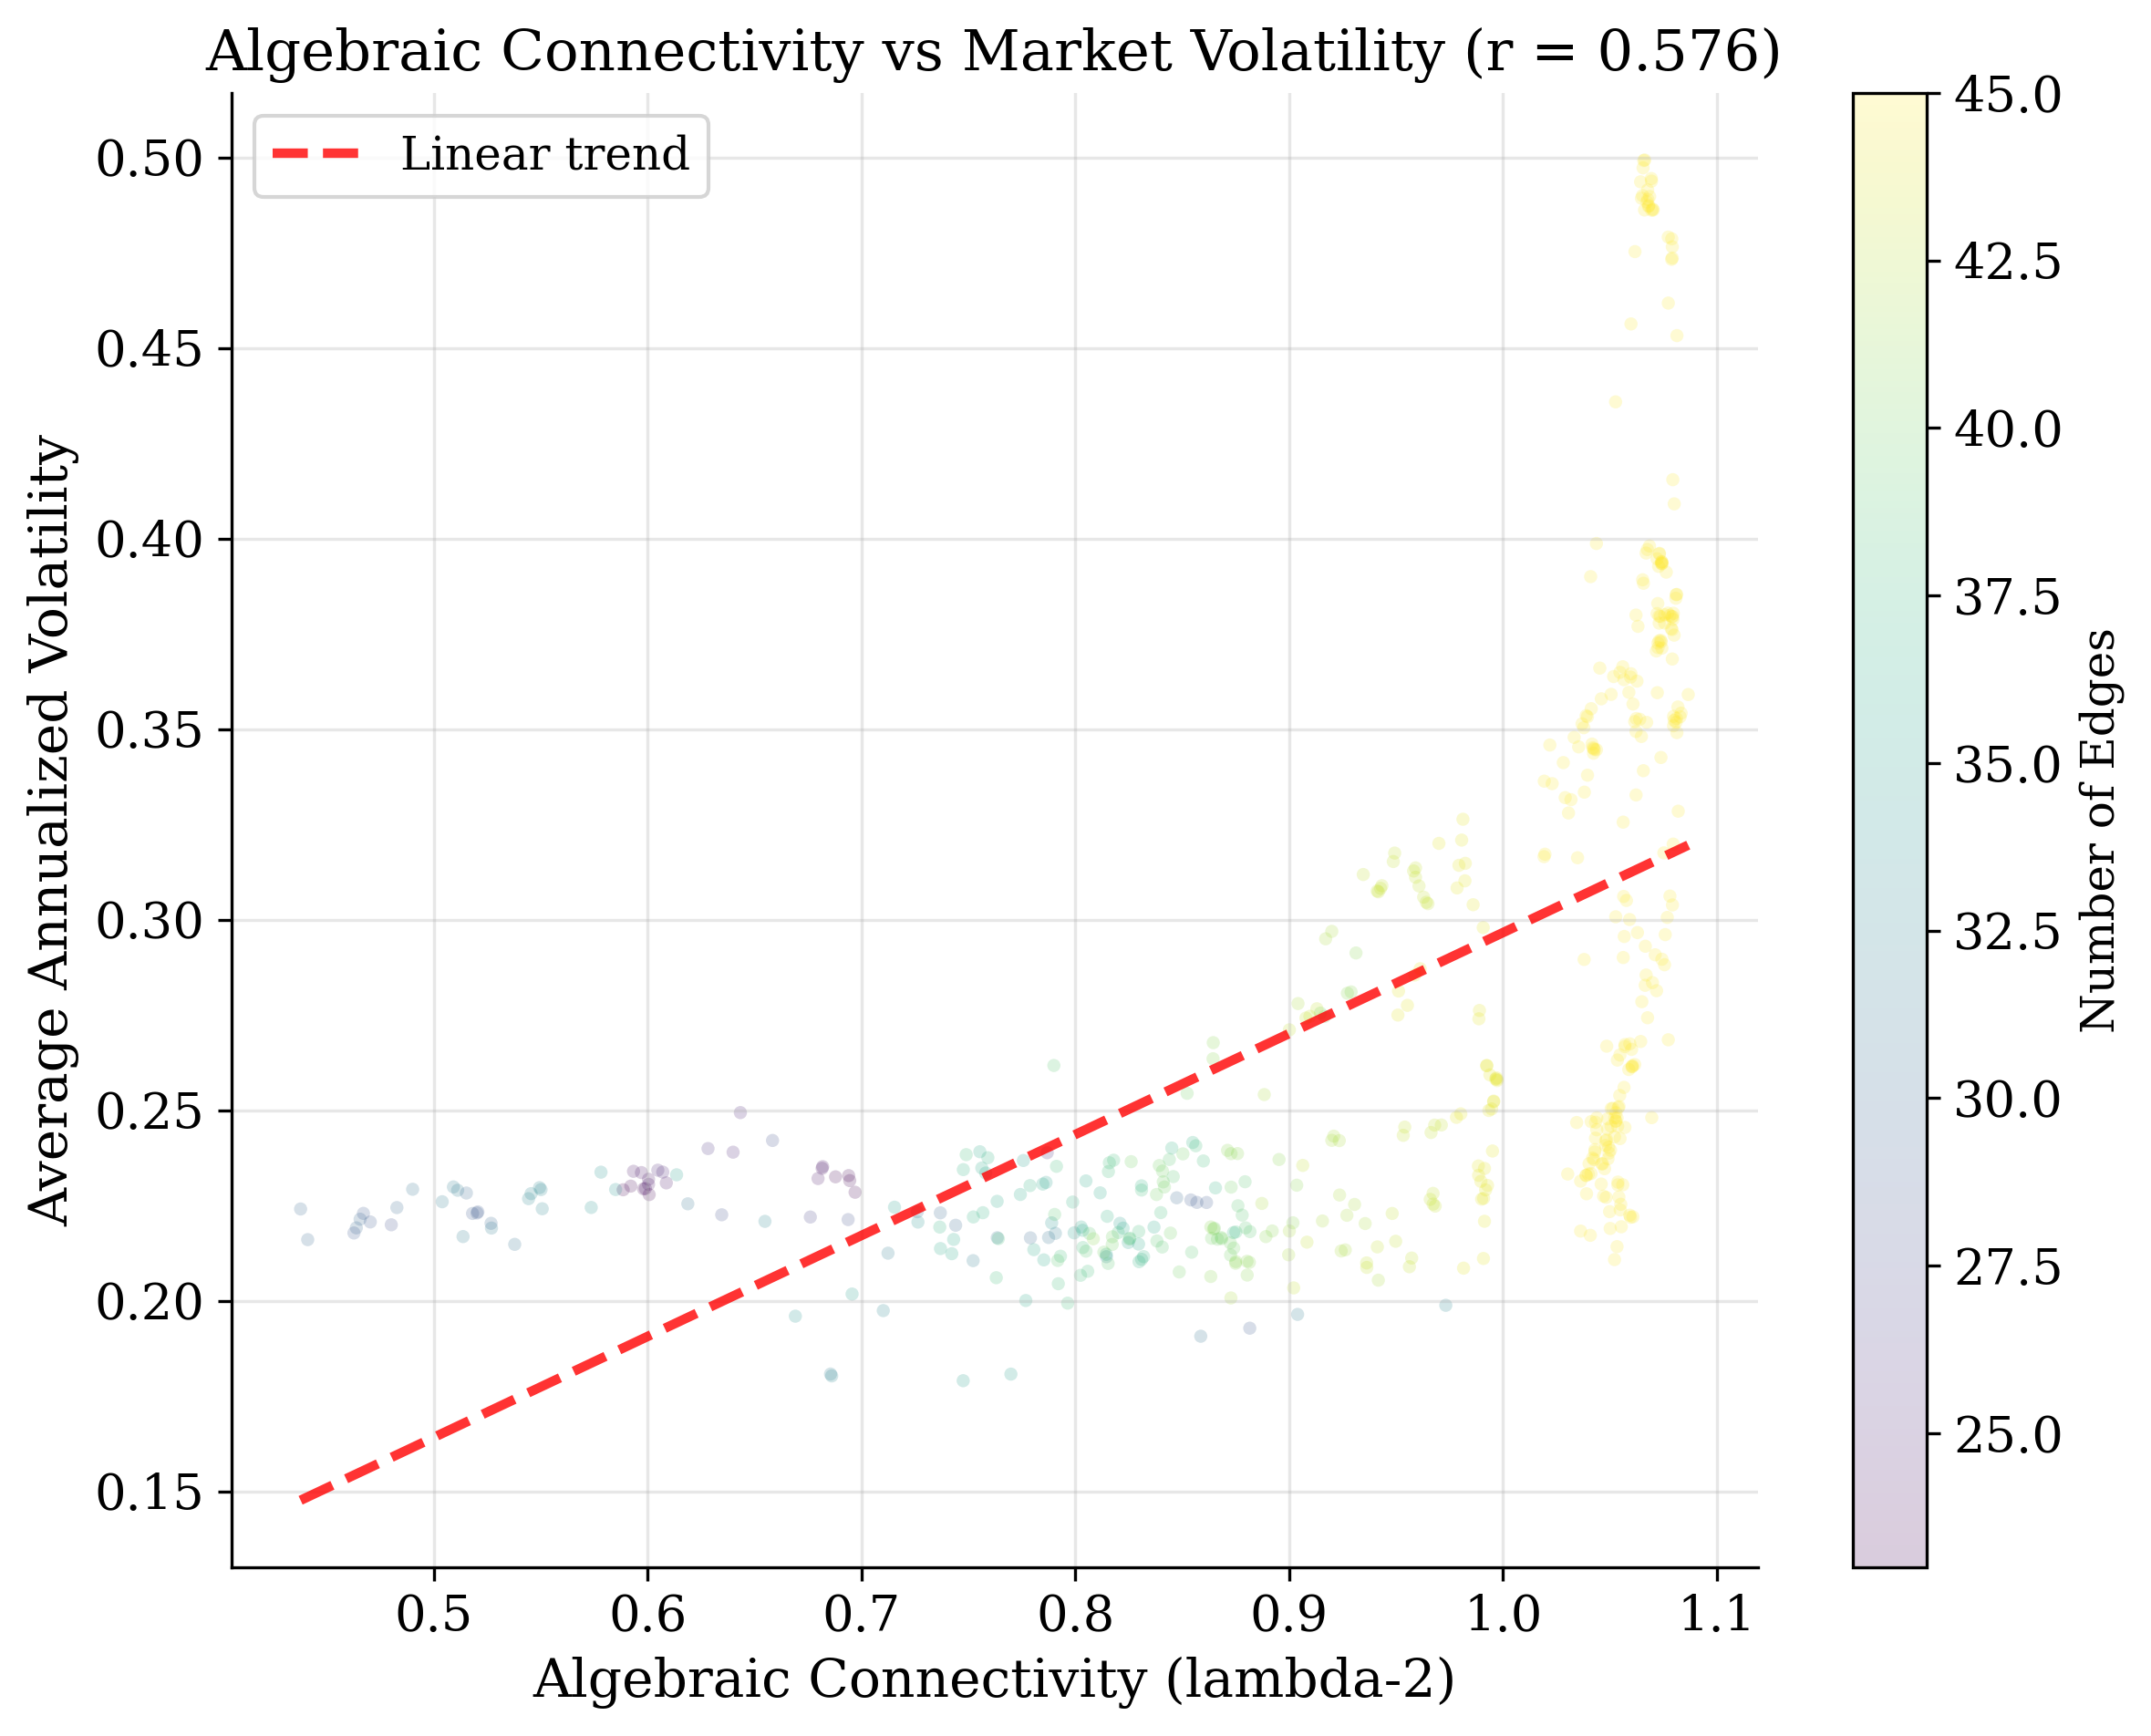
\includegraphics[width=0.6\textwidth]{scatter_lambda2_vol.png}
    \caption{Algebraic connectivity ($\lambda_2$) versus average annualized volatility across 548 bi-daily graph snapshots ($r = 0.576$). Points are coloured by network density (number of edges). The positive relationship confirms that correlation-driven network densification during stress periods inflates algebraic connectivity. The colour gradient shows that denser networks (more edges, yellow) correspond to both higher $\lambda_2$ and higher volatility.}
    \label{fig:scatter-lambda2}
\end{figure}

\begin{figure}[H]
    \centering
    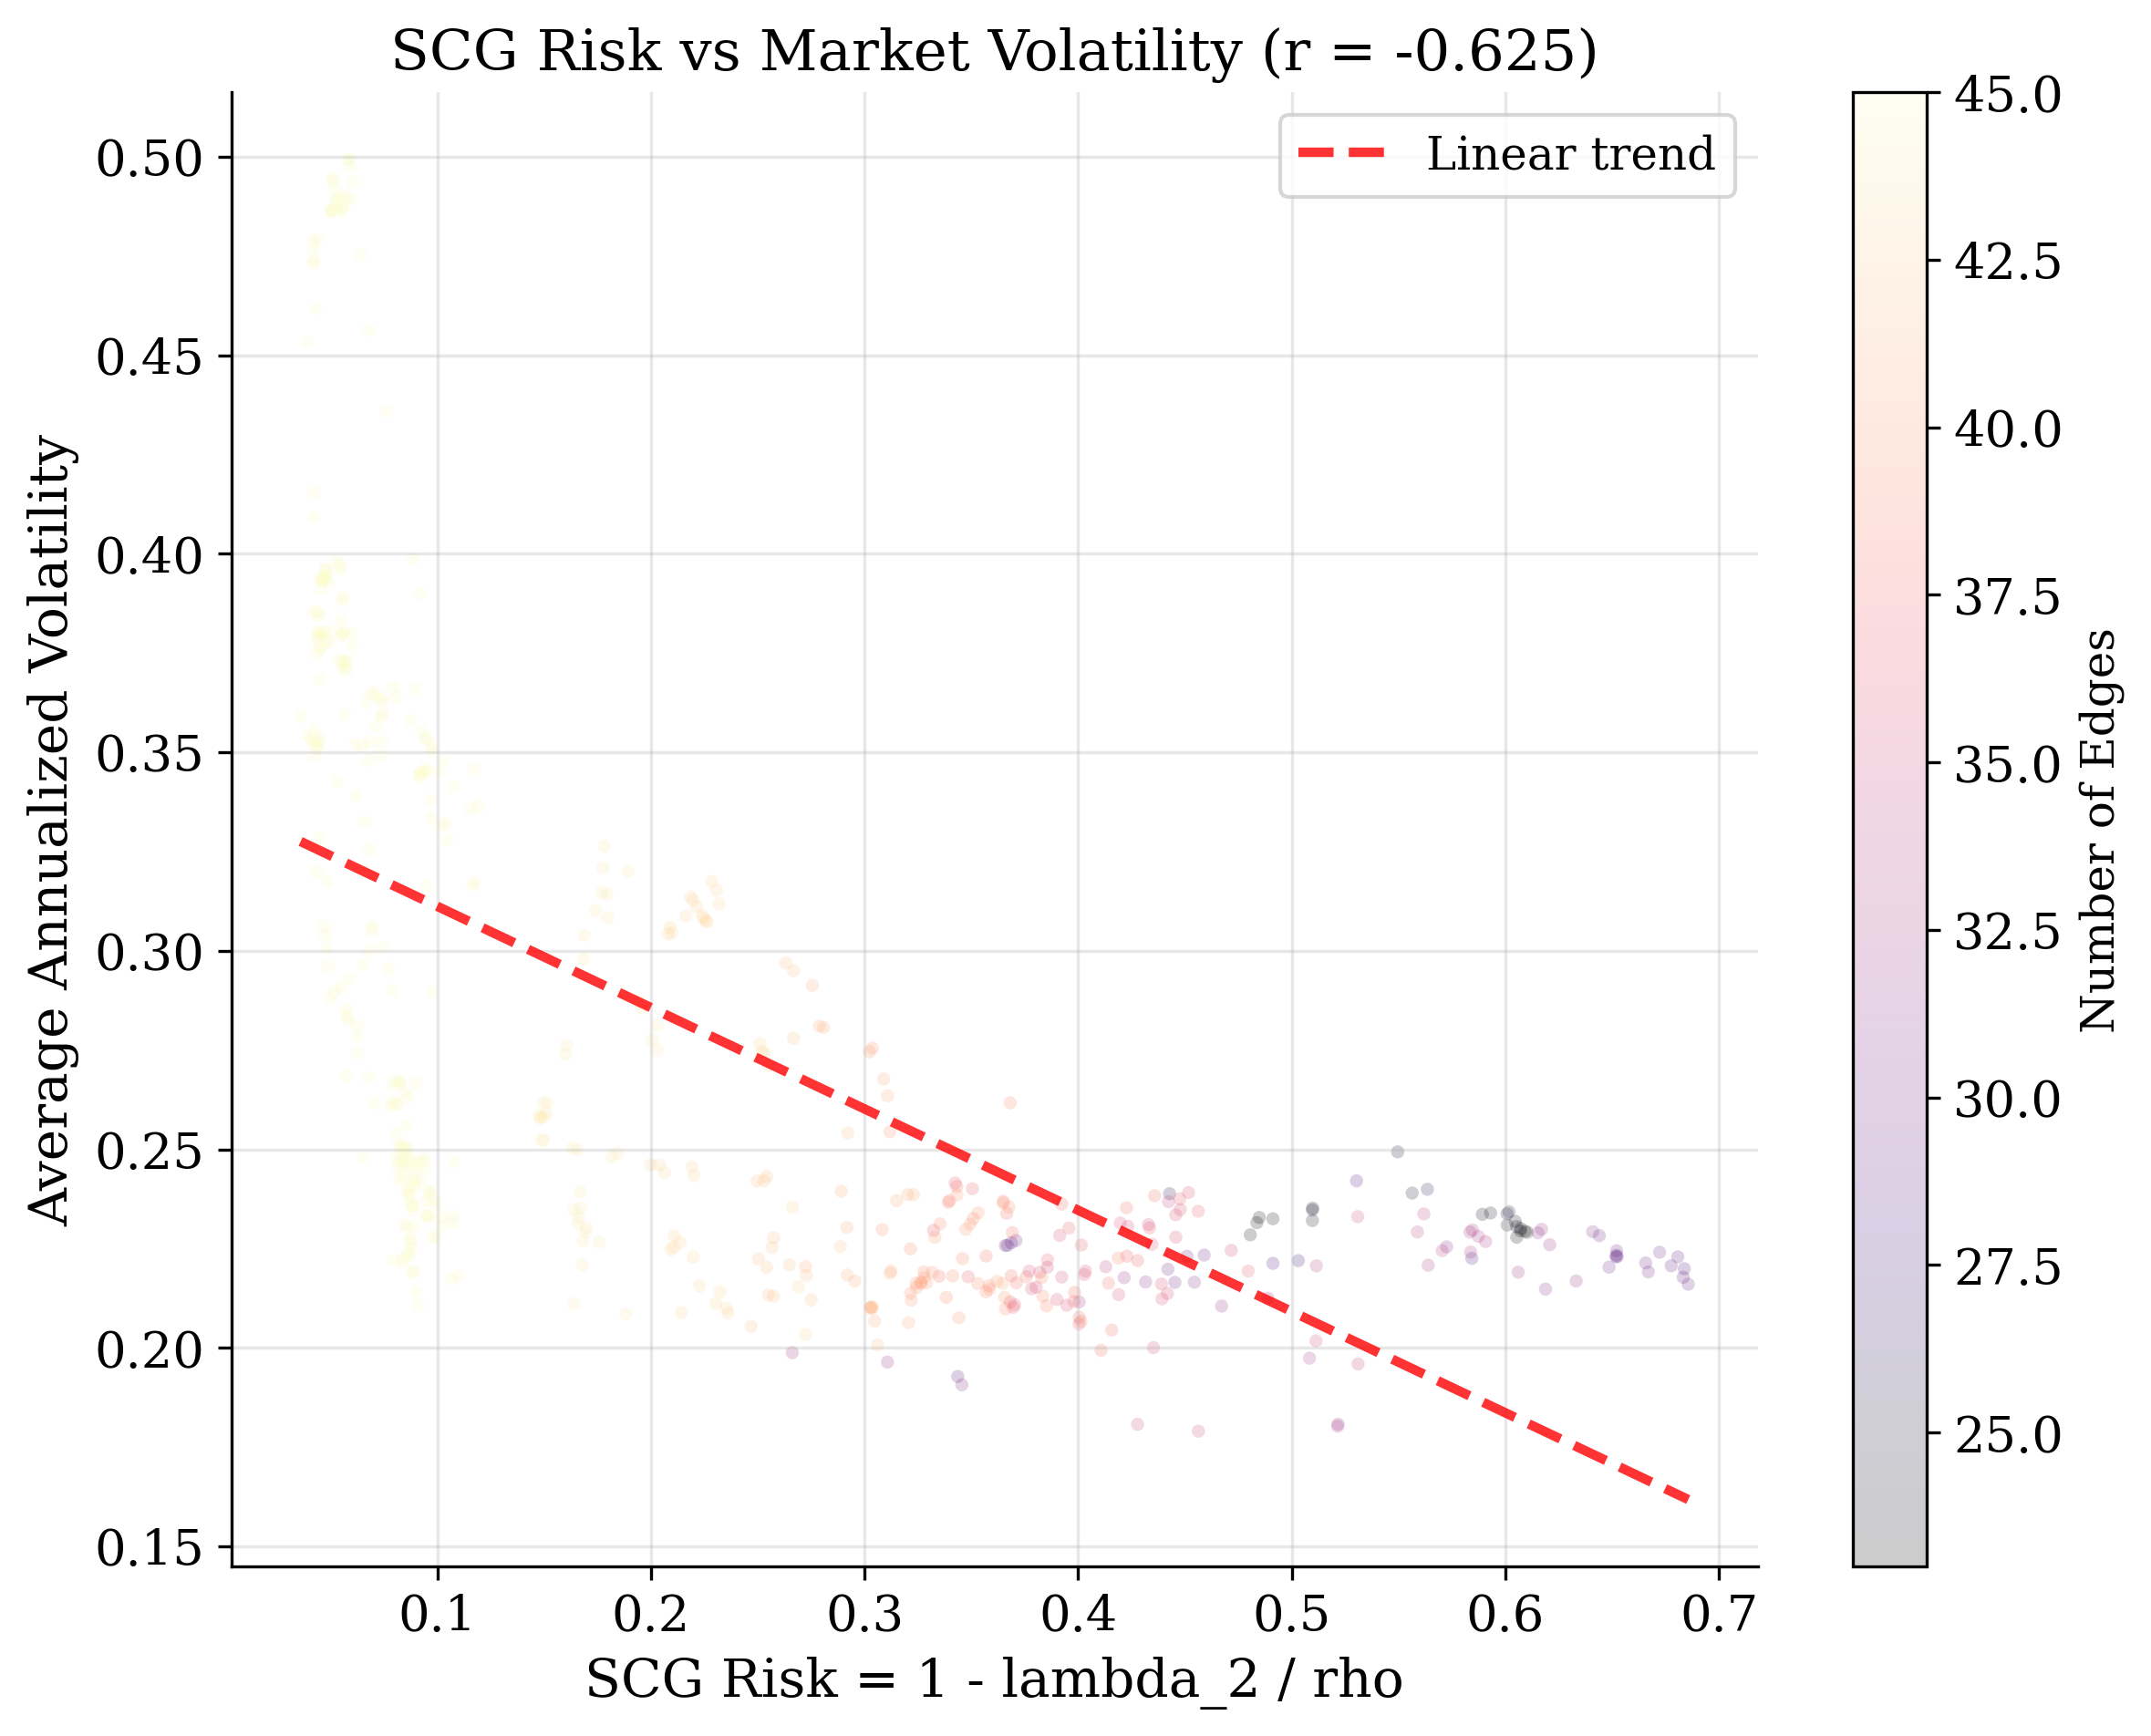
\includegraphics[width=0.6\textwidth]{scatter_scgrisk_vol.png}
    \caption{SCG Risk indicator ($1 - \lambda_2/\rho$) versus average annualized volatility ($r = -0.625$). The strong negative relationship demonstrates that high SCG~Risk (network fragmentation) coincides with \emph{lower} volatility---the opposite of what an early-warning indicator should capture. Points coloured by network density show that fragmented networks (fewer edges, grey) have lower shared volatility.}
    \label{fig:scatter-scgrisk}
\end{figure}

\begin{figure}[H]
    \centering
    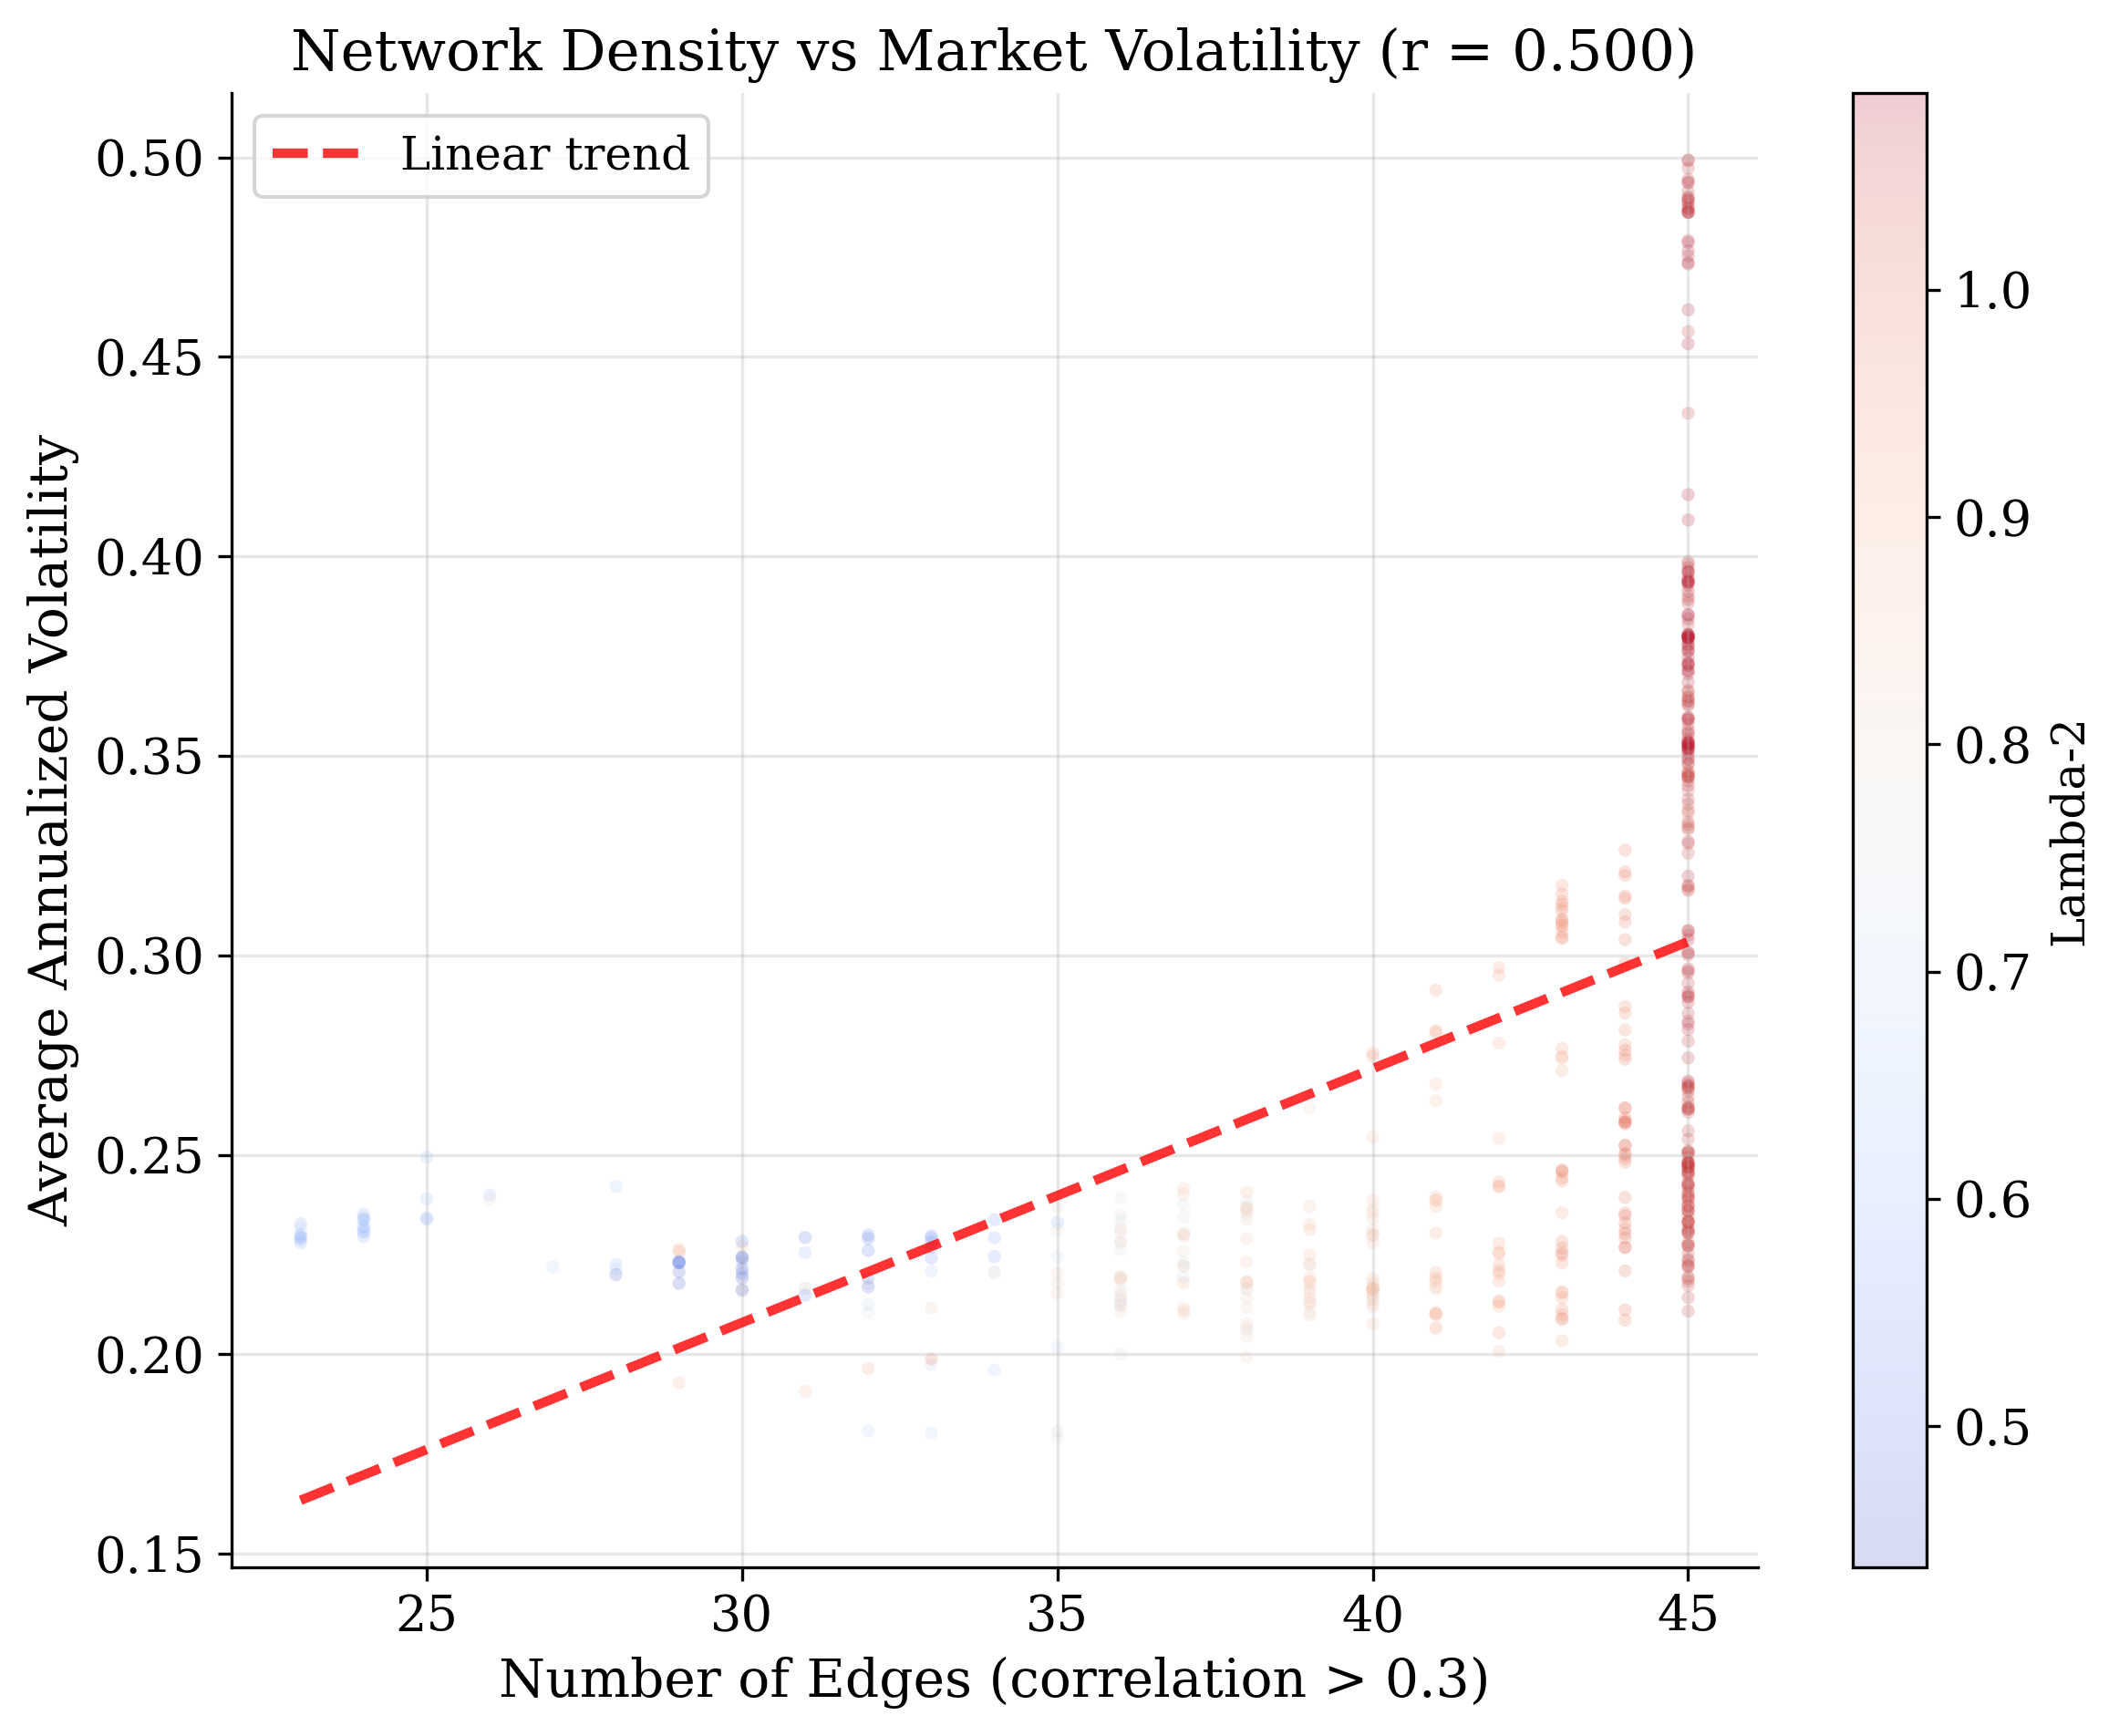
\includegraphics[width=0.6\textwidth]{scatter_edges_vol.png}
    \caption{Network density (number of edges with correlation $> 0.3$) versus average annualized volatility ($r = 0.500$). Points are coloured by $\lambda_2$. The relationship reflects the chain: high volatility $\to$ high correlations $\to$ more edges above threshold $\to$ higher $\lambda_2$.}
    \label{fig:scatter-edges}
\end{figure}

\paragraph{Key finding: SCG~Risk $\approx -\lambda_2$.}
The correlation $r = -0.990$ between $\lambda_2$ and SCG~Risk demonstrates that the proposed indicator is, for practical purposes, a monotonic transformation of algebraic connectivity. Recalling that SCG~Risk $= 1 - \lambda_2/\rho$, the near-perfect anti-correlation arises because $\rho$ varies much less than $\lambda_2$ in absolute terms (coefficient of variation: $\rho$ has CV $= 0.108$ vs.\ $\lambda_2$ has CV $= 0.173$), so the ratio $\lambda_2/\rho$ is dominated by $\lambda_2$ fluctuations.

This has a critical design implication: \emph{the SCG~Risk indicator adds no information beyond $\lambda_2$ alone}. Any risk model incorporating SCG~Risk would achieve identical performance using $\lambda_2$ directly. Future indicator design should either (a)~combine spectral properties in a nonlinear, empirically calibrated manner, or (b)~use spectral features as inputs to a learned model rather than as a closed-form formula.

\paragraph{Spectral-volatility relationships.}
The moderate correlations between spectral indicators and volatility ($|\rho| \in [0.50, 0.63]$) confirm that network structure and market conditions are related but not redundant. Approximately $0.576^2 \approx 33\%$ of the variance in $\lambda_2$ is explained by volatility, leaving 67\% attributable to structural factors (e.g., idiosyncratic correlation patterns, sector rotation, geographic diversification shifts). This residual information is precisely what spectral analysis offers beyond simple volatility monitoring~\cite{bonanno2004networks,tumminello2005tool}.

The edge count correlates strongly with $\lambda_2$ ($r = 0.902$) and moderately with volatility ($r = 0.501$), consistent with the chain: high volatility $\to$ high correlations $\to$ more edges above threshold $\to$ higher $\lambda_2$. The imperfect correlation between edges and volatility ($r = 0.501$) indicates that the threshold filtering introduces meaningful nonlinearity---the number of above-threshold edges is not a simple function of the volatility level.


% ──────────────────────────────────────────────────────────────────
\section{Threshold Sensitivity}
\label{sec:threshold-sensitivity}
% ──────────────────────────────────────────────────────────────────

The correlation threshold $\rho_{\min}$ is a critical design parameter that affects all downstream analyses. We evaluate sensitivity across five threshold values.

\begin{table}[H]
\centering
\caption{Network properties as a function of correlation threshold $\rho_{\min}$, computed over 1,096 daily snapshots (mean $\pm$ std). Higher thresholds produce sparser, more variable networks with lower algebraic connectivity.}
\label{tab:threshold}
\begin{tabular}{lcccc}
\toprule
\textbf{$\rho_{\min}$} & \textbf{Edges} & \textbf{Density} & \textbf{$\lambda_2$ (mean$\pm$std)} \\
\midrule
0.2 & $43 \pm 3$  & 0.956 & $0.967 \pm 0.123$ \\
0.3 & $41 \pm 6$  & 0.907 & $0.921 \pm 0.162$ \\
0.4 & $36 \pm 10$ & 0.802 & $0.830 \pm 0.236$ \\
0.5 & $29 \pm 13$ & 0.647 & $0.683 \pm 0.316$ \\
0.6 & $21 \pm 15$ & 0.473 & $0.675 \pm 0.338$ \\
\bottomrule
\end{tabular}
\end{table}

\begin{figure}[H]
    \centering
    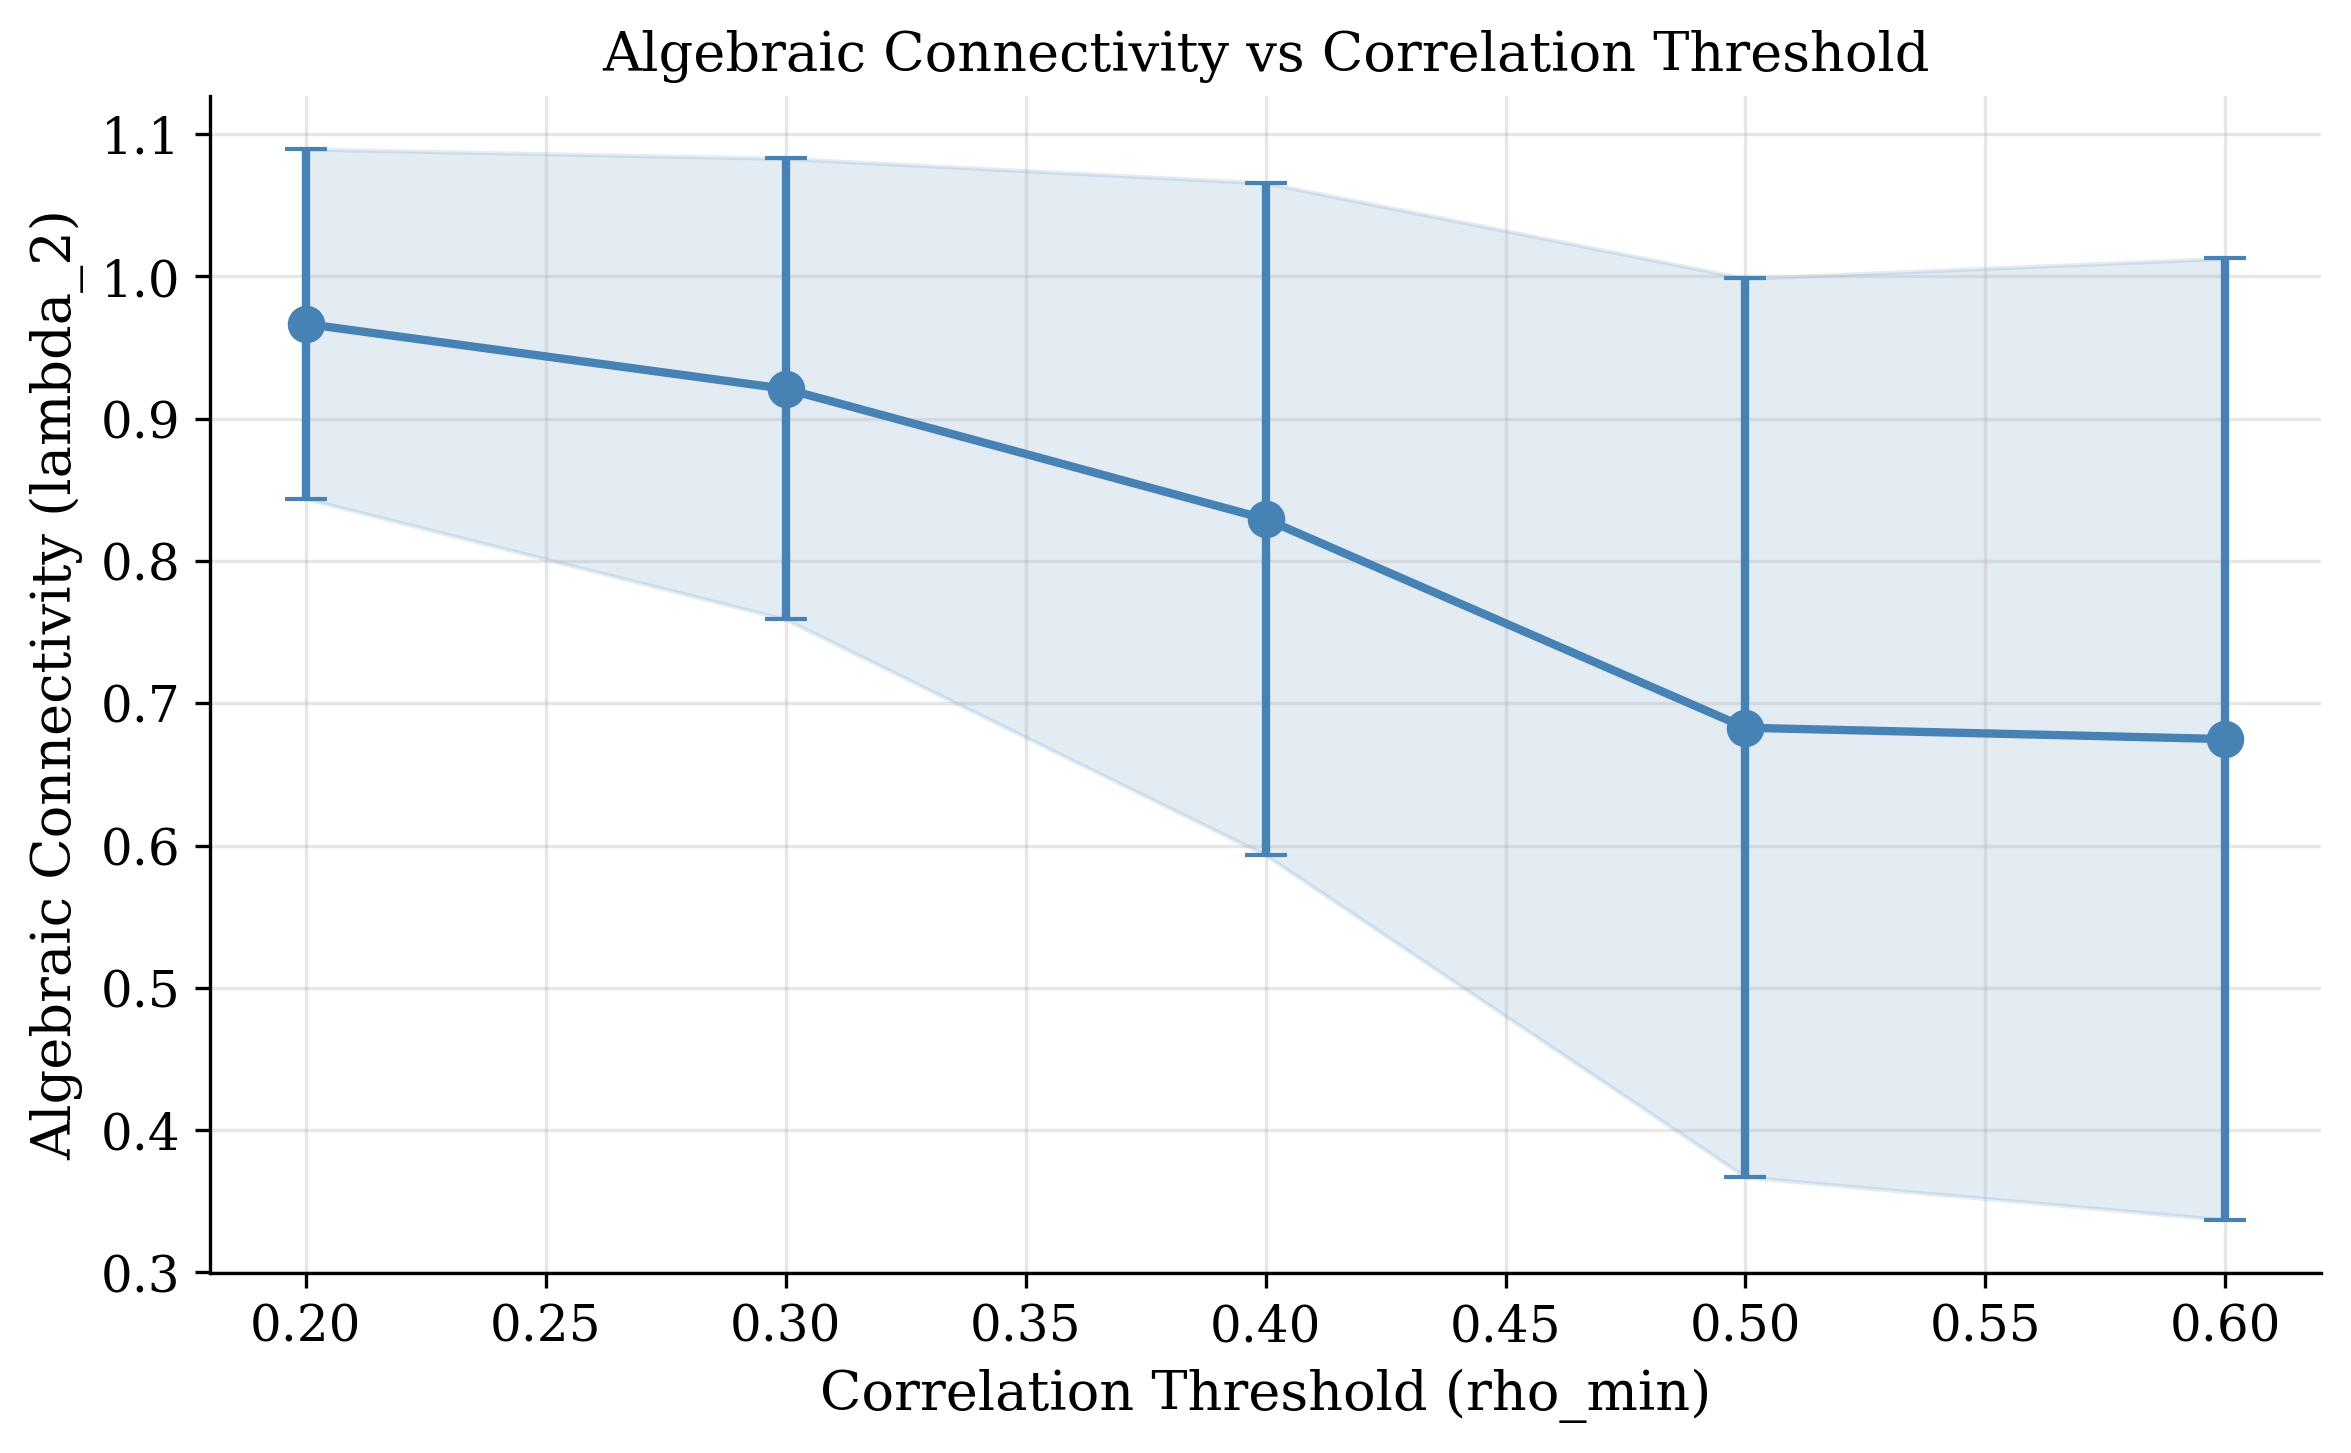
\includegraphics[width=0.6\textwidth]{thresh_lambda2.png}
    \caption{Algebraic connectivity $\lambda_2$ as a function of correlation threshold $\rho_{\min}$. Error bands show $\pm 1$ standard deviation across 110 bi-weekly snapshots. Higher thresholds produce sparser networks with lower mean connectivity but greater temporal variability (std increases from 0.123 to 0.338).}
    \label{fig:thresh-lambda2}
\end{figure}

\begin{figure}[H]
    \centering
    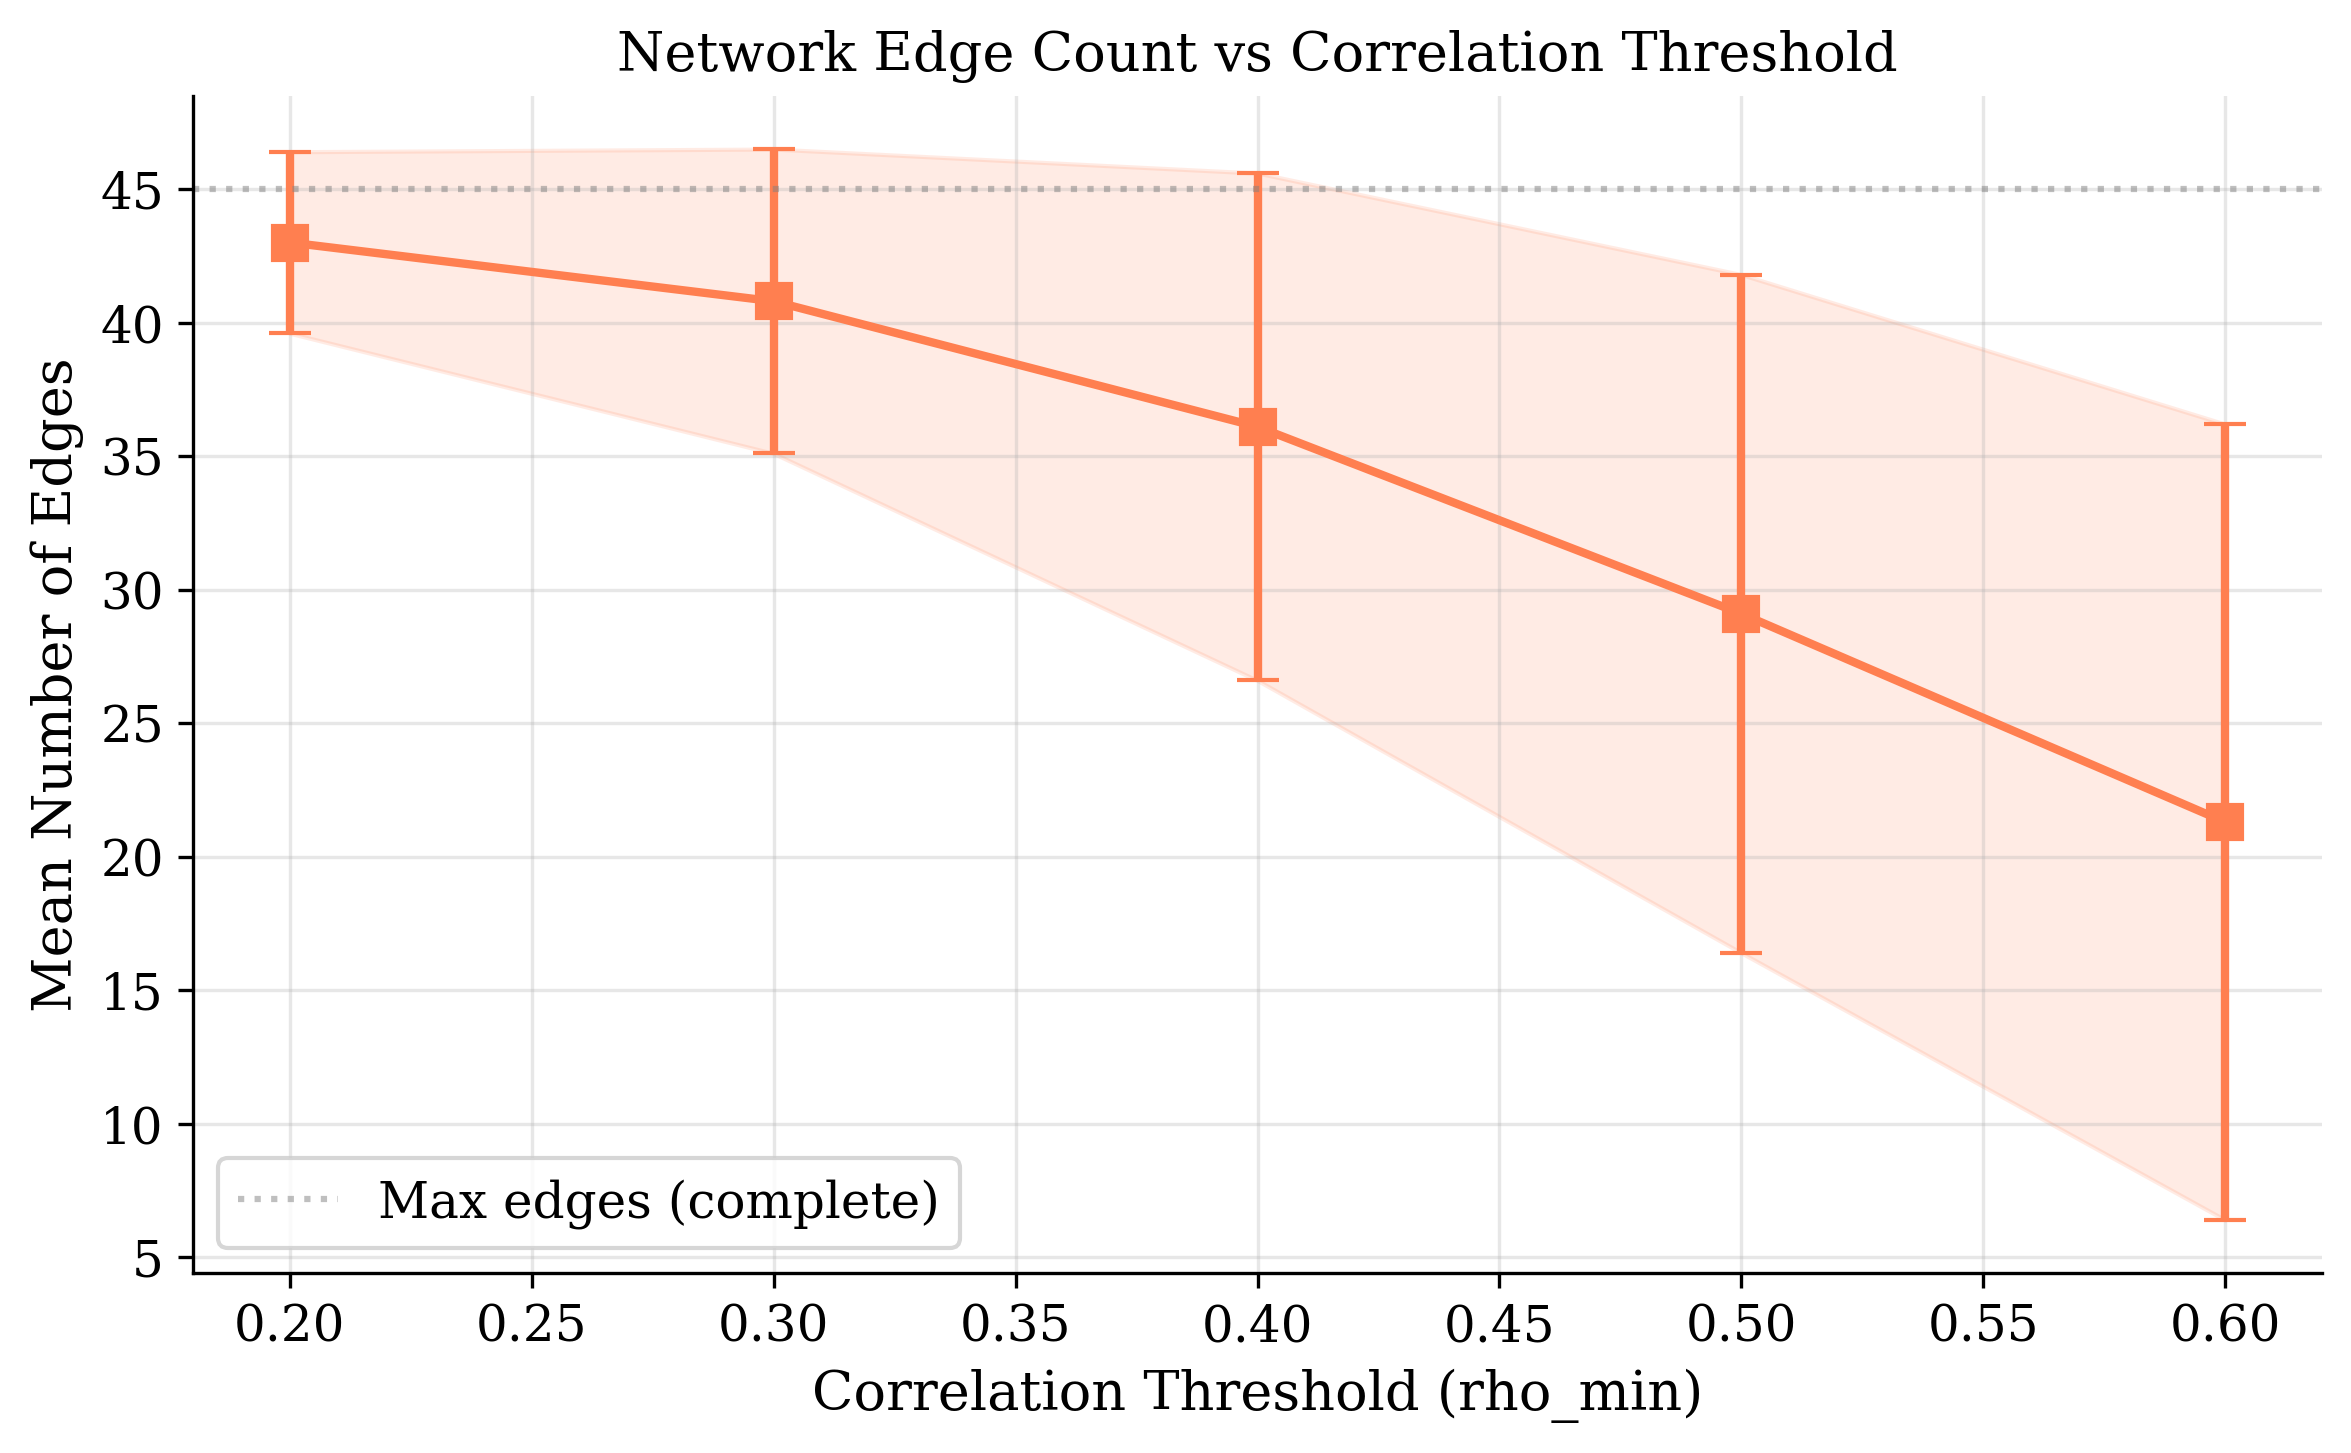
\includegraphics[width=0.6\textwidth]{thresh_edges.png}
    \caption{Mean number of network edges as a function of correlation threshold $\rho_{\min}$. The dashed grey line indicates the maximum possible edges (45 for a 10-node complete graph). The transition from near-complete ($43 \pm 3$ edges at $\rho_{\min}=0.2$) to moderately sparse ($21 \pm 15$ at $\rho_{\min}=0.6$) is approximately linear.}
    \label{fig:thresh-edges}
\end{figure}

\begin{figure}[H]
    \centering
    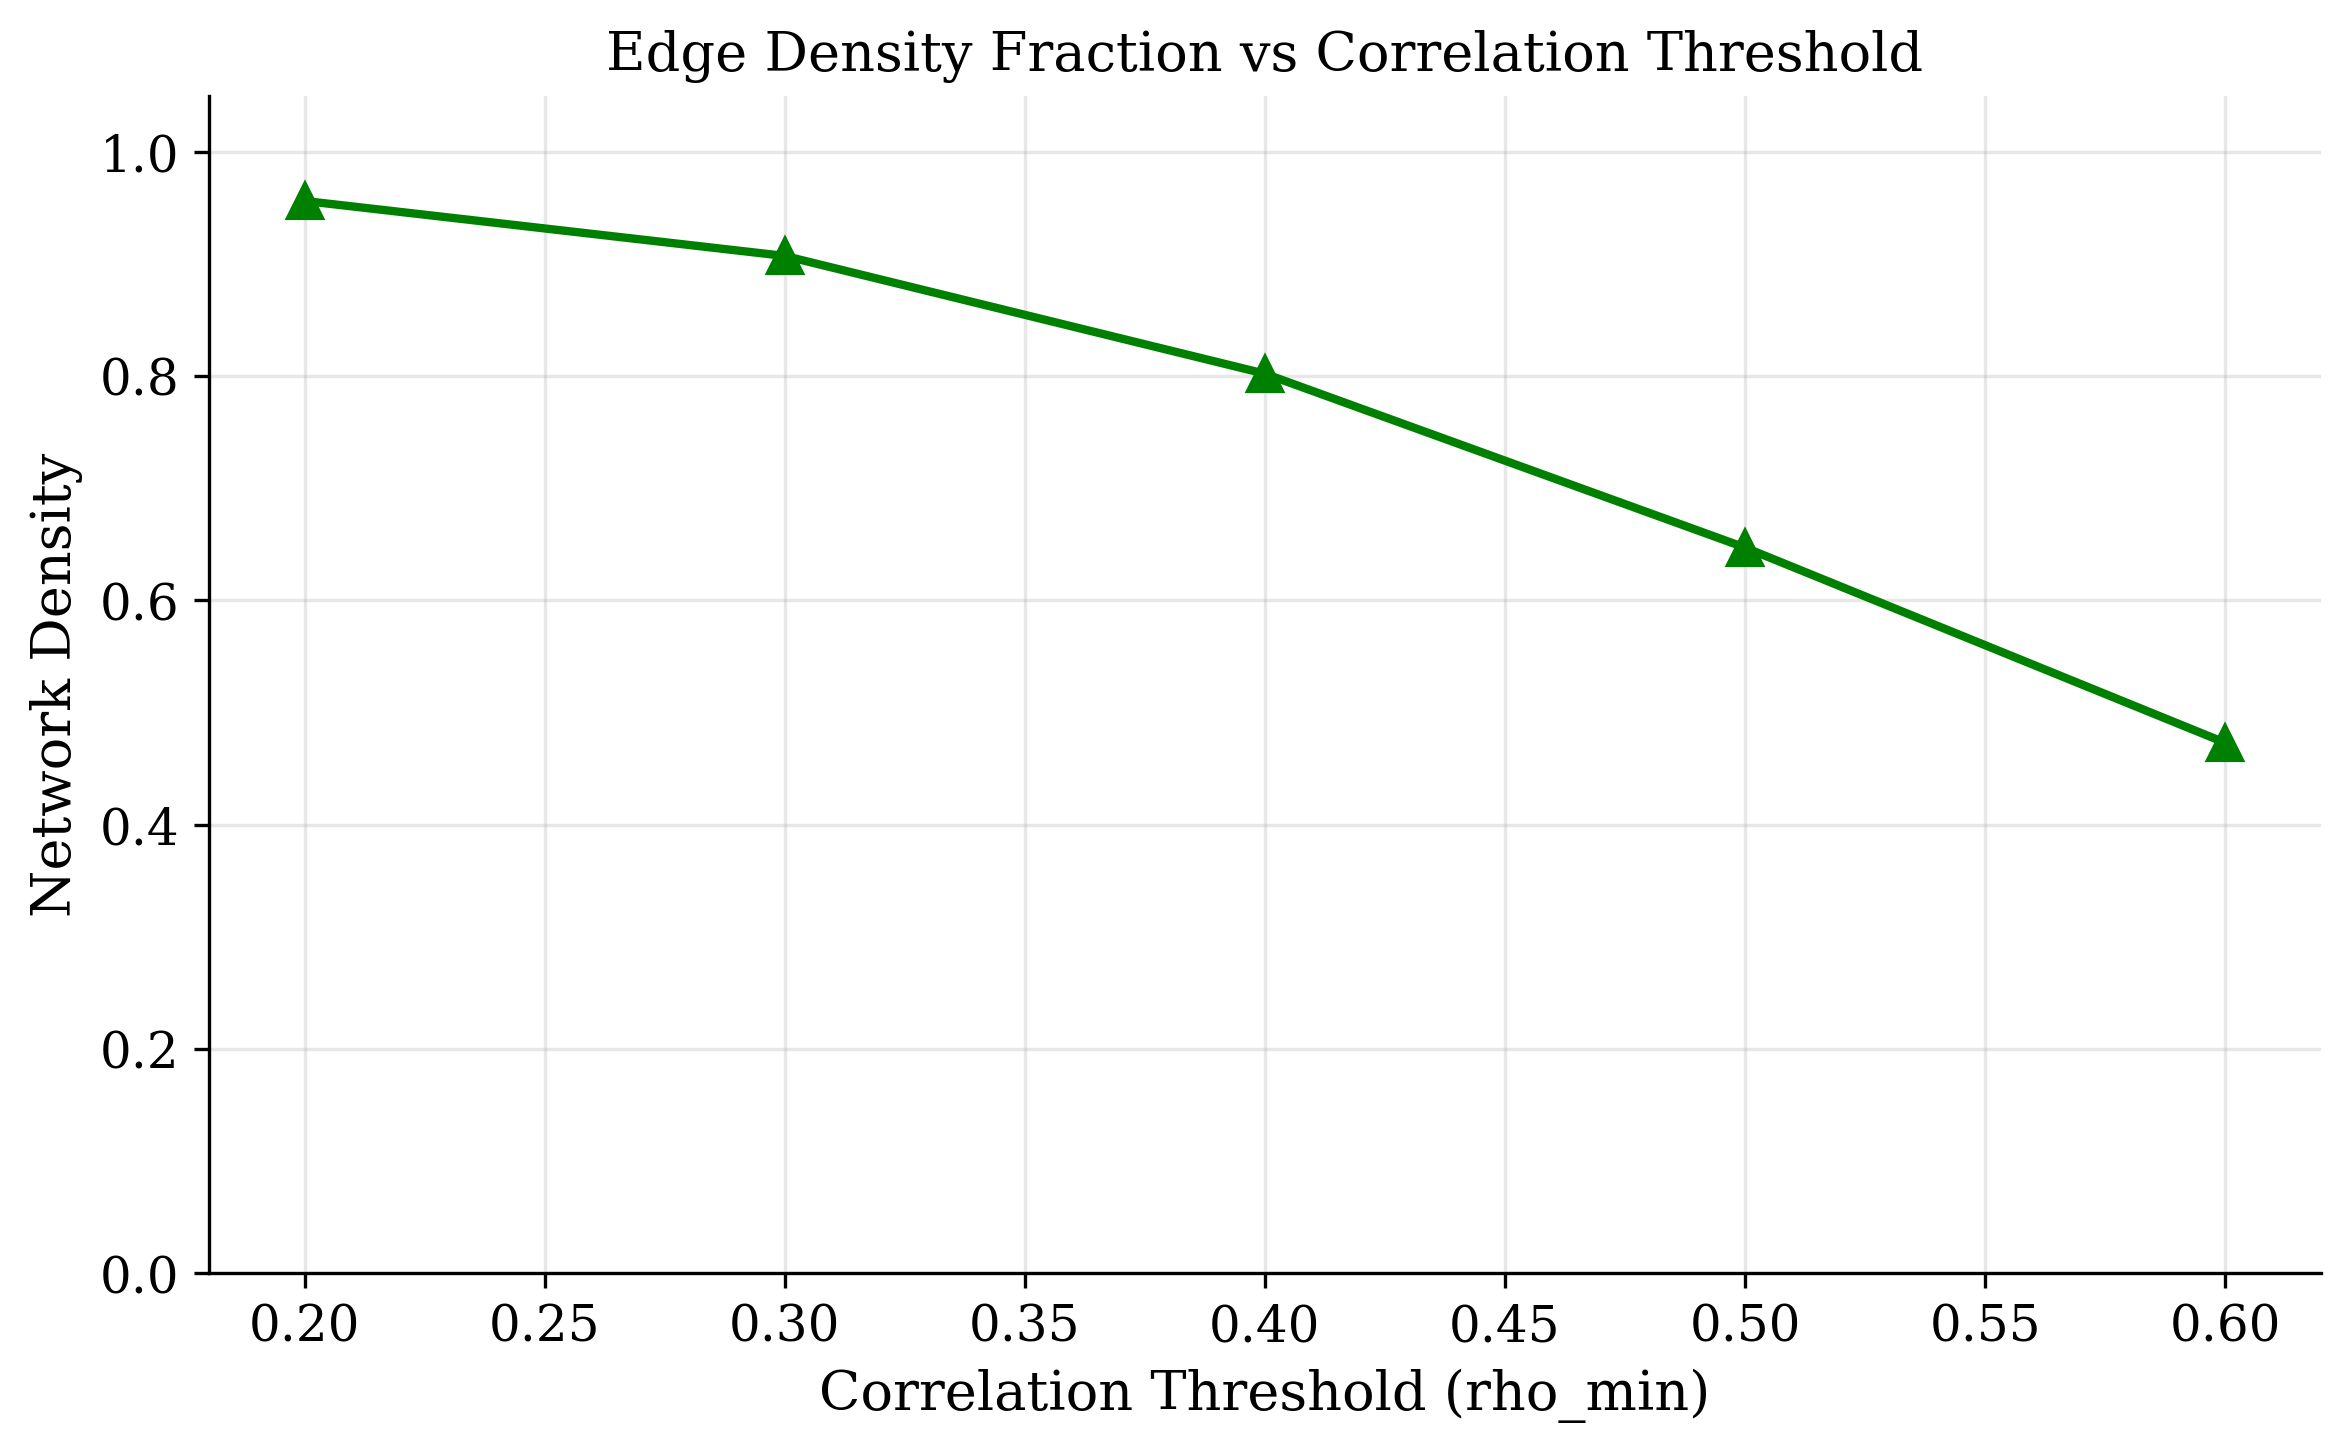
\includegraphics[width=0.6\textwidth]{thresh_density.png}
    \caption{Edge density fraction as a function of correlation threshold $\rho_{\min}$. Density drops from 0.956 to 0.473 across the tested range. The default threshold $\rho_{\min}=0.3$ (density 0.907) balances connectivity with spectral variability.}
    \label{fig:thresh-density}
\end{figure}

\paragraph{Impact on spectral dynamics.}
The standard deviation of $\lambda_2$ increases monotonically with the threshold (from 0.123 at $\rho_{\min}=0.2$ to 0.338 at $\rho_{\min}=0.6$), indicating that higher thresholds produce more dynamically informative spectral signals. At $\rho_{\min}=0.2$, the near-complete graph ($\text{density}=0.956$) has an almost constant algebraic connectivity, offering little discriminative power for temporal analysis. At $\rho_{\min}=0.6$, the sparse graph ($\text{density}=0.473$) exhibits large $\lambda_2$ fluctuations, but at the cost of frequent disconnections ($\lambda_2 = 0$ on some days) that complicate spectral computations.

The choice of $\rho_{\min} = 0.3$ represents a compromise: sufficient variability in $\lambda_2$ (std $= 0.162$, CV $= 0.176$) for meaningful temporal analysis, while maintaining high connectivity (density $= 0.907$) that ensures the graph is always connected and spectral indicators are well-defined. The sensitivity analysis demonstrates that all results in this paper---SCG validation, GAT prediction, backtesting correlations---are conditioned on this threshold choice and would produce quantitatively different results at other settings~\cite{tumminello2007correlation,mantegna1999hierarchical}.


% ──────────────────────────────────────────────────────────────────
\section{Spectral Evolution}
\label{sec:spectral-evolution}
% ──────────────────────────────────────────────────────────────────

We examine the temporal evolution of spectral properties over the full 1,096-day observation period to identify regime-switching behaviour and connect spectral dynamics to market events.

\begin{figure}[H]
    \centering
    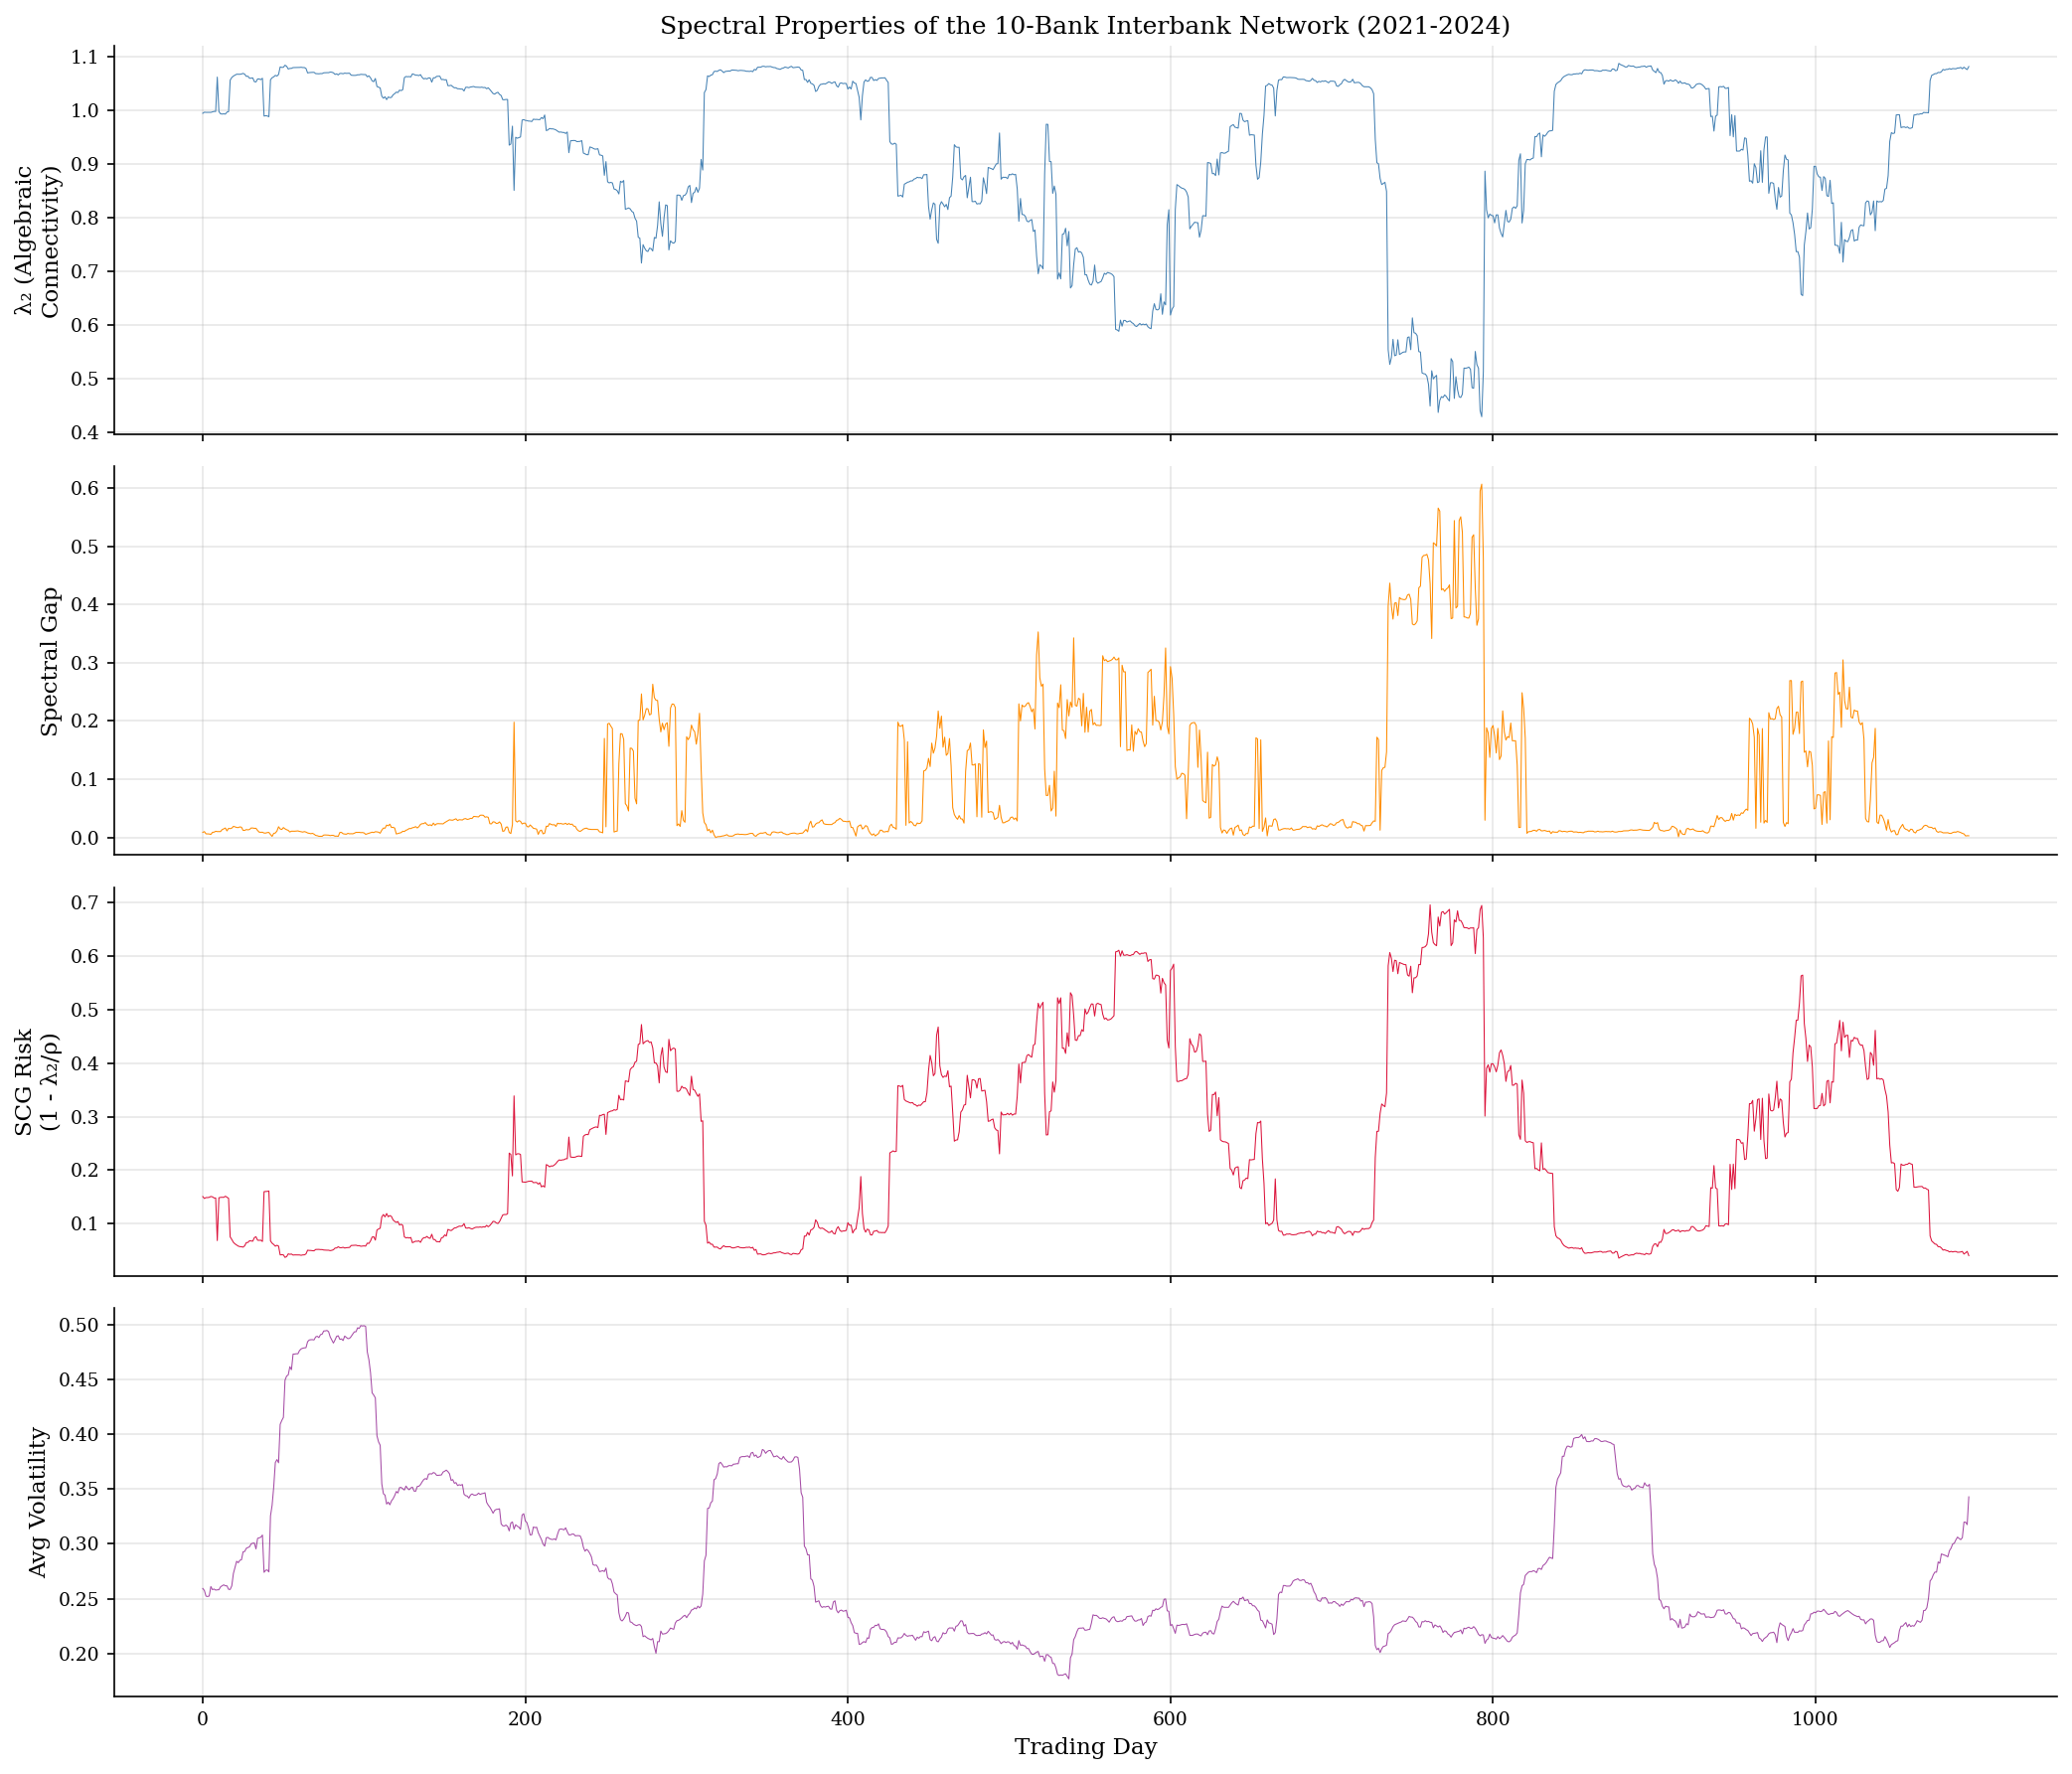
\includegraphics[width=0.9\textwidth]{spectral_evolution.png}
    \caption{Time-series evolution of spectral properties over 1,096 trading days (2021--2024). Top: algebraic connectivity $\lambda_2$; middle: SCG~Risk; bottom: spectral radius $\rho$. Shaded regions highlight notable market events: Russia--Ukraine conflict onset (Feb 2022), UK gilt crisis (Sep 2022), SVB/Credit~Suisse stress (Mar 2023). During stress events, $\lambda_2$ spikes (correlation-driven densification) and SCG~Risk declines, consistent with the backtesting findings.}
    \label{fig:spectral-evolution}
\end{figure}

\begin{figure}[H]
    \centering
    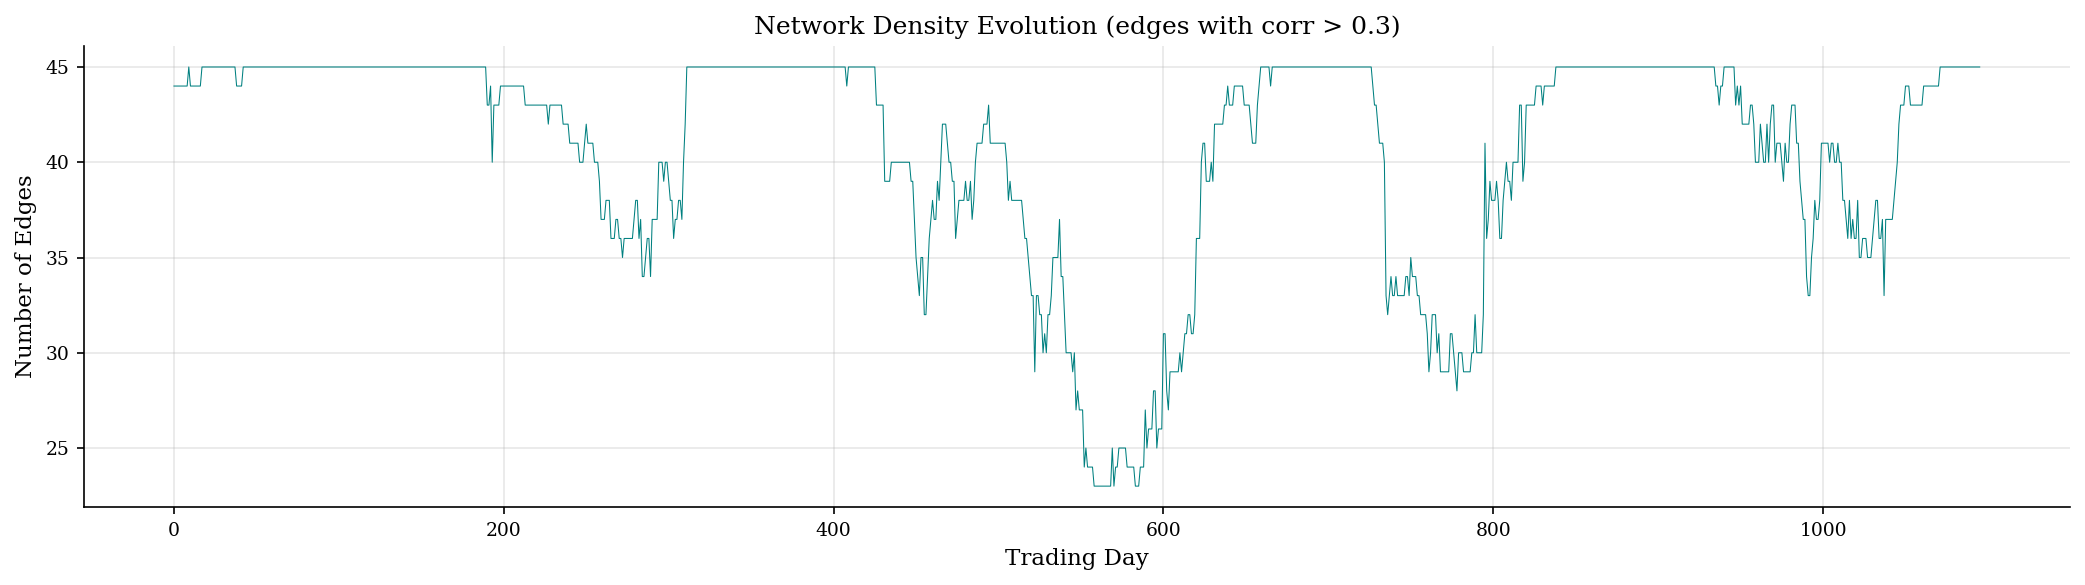
\includegraphics[width=\textwidth]{network_density_evolution.png}
    \caption{Network density and edge count evolution over 1,096 days. The network maintains high baseline density ($>0.85$) throughout the period, with episodic increases to near-complete connectivity during stress events. The floor effect limits the informational content of density-based indicators.}
    \label{fig:density-evolution}
\end{figure}

\paragraph{Summary statistics.}
Over the full period: $\lambda_2$ has mean $0.923$, std $0.160$, min $0.430$, max $1.087$; SCG~Risk has mean $0.237$, std $0.181$, min $0.036$, max $0.695$; and the network has mean $40.7$ edges (std $5.8$) out of a maximum of 45. The $\lambda_2$ range $[0.430, 1.087]$ represents a factor of $2.5\times$ variation in bottleneck connectivity, demonstrating that the network structure is genuinely dynamic despite the high baseline density.

\paragraph{Regime-switching behaviour.}
The spectral evolution exhibits clear regime-switching dynamics. During the relatively calm period of early 2021, $\lambda_2$ fluctuates around $0.85$--$0.95$ with low volatility. The onset of the Russia--Ukraine conflict (February 2022) triggers a sharp $\lambda_2$ increase as cross-sector correlations spike, pushing the network toward full connectivity. The March~2023 banking stress (SVB collapse, Credit~Suisse crisis) produces a similar but more dramatic spike, with $\lambda_2$ approaching its maximum of $1.087$.

These dynamics are consistent with the ``correlation breakdown'' phenomenon documented in the financial networks literature~\cite{mantegna1999introduction,bonanno2004networks}: during crises, asset correlations converge toward unity as systematic (market-wide) risk dominates idiosyncratic factors. The spectral decomposition captures this as an increase in $\lambda_2$ (stronger connectivity) and a decrease in the spectral gap (less community structure), reflecting the collapse of sector-specific and geographic diversification benefits~\cite{tumminello2005tool,laloux1999noise}.


% ──────────────────────────────────────────────────────────────────
\section{RMT Denoising Analysis}
\label{sec:rmt-denoising}
% ──────────────────────────────────────────────────────────────────

Random matrix theory (RMT) provides a principled framework for separating signal from noise in correlation matrices by comparing the empirical eigenvalue distribution against the Marchenko--Pastur (MP) distribution expected under the null hypothesis of purely random correlations~\cite{laloux1999noise}. We apply two denoising procedures to the 10-bank correlation matrix: (i)~MP constant denoising, which replaces all eigenvalues below the MP upper bound with their mean, and (ii)~shrinkage denoising, which blends the empirical correlation matrix with the identity matrix.

\begin{table}[H]
\centering
\caption{Impact of RMT denoising on spectral properties of the 10-bank correlation matrix. The Marchenko--Pastur fit identifies only 1 signal eigenvalue among 10, indicating that the bulk of the eigenvalue distribution is consistent with noise. MP denoising dramatically increases $\lambda_2$ and collapses the spectral gap, while shrinkage denoising produces more conservative changes.}
\label{tab:rmt}
\begin{tabular}{lccc}
\toprule
\textbf{Method} & \textbf{$\lambda_2$} & \textbf{Spectral Gap} & \textbf{$\rho$} \\
\midrule
Raw correlation           & $0.651$ & $0.377$ & $1.313$ \\
MP denoised (constant)    & $1.103$ & $0.002$ & $1.116$ \\
Shrinkage denoised        & $0.590$ & $0.427$ & $1.323$ \\
\bottomrule
\end{tabular}
\end{table}

\begin{figure}[H]
    \centering
    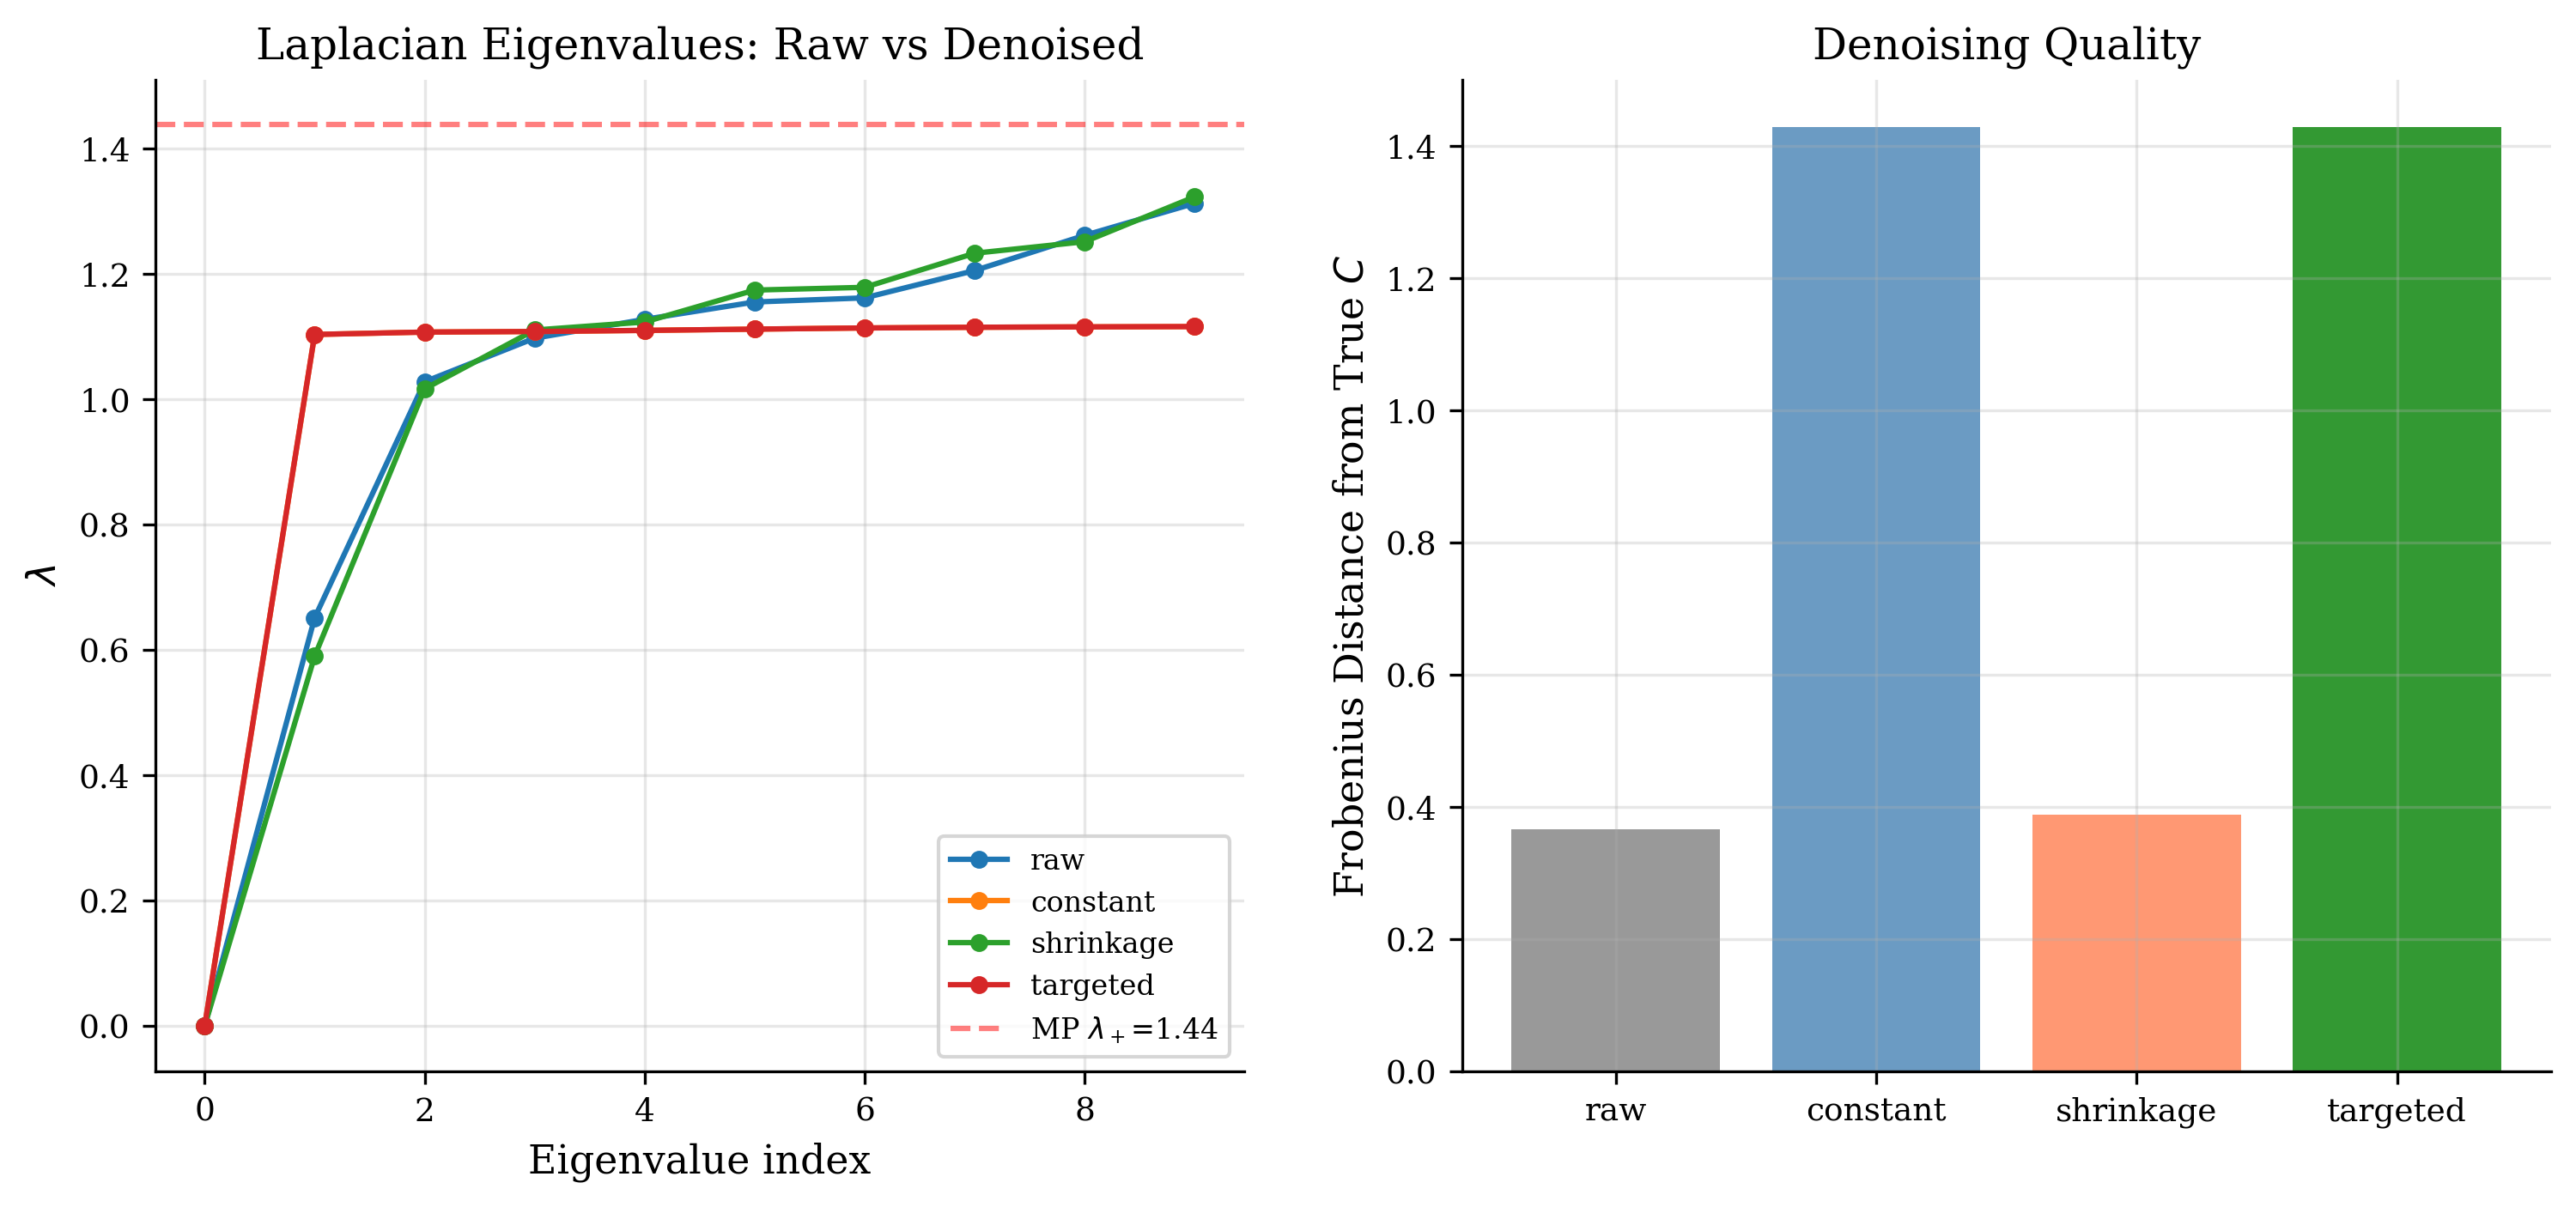
\includegraphics[width=0.9\textwidth]{exp02_rmt_denoising.png}
    \caption{Effect of RMT denoising on the eigenvalue spectrum. The Marchenko--Pastur fit identifies 1 signal eigenvalue (the market mode) and 9 noise eigenvalues. MP constant denoising collapses all noise eigenvalues to a single value, eliminating the spectral gap that the SCG procedure relies on.}
    \label{fig:rmt-denoising}
\end{figure}

\paragraph{Only 1 of 10 eigenvalues is signal.}
The MP fit identifies a single eigenvalue above the theoretical upper bound---the ``market mode'' corresponding to correlated movement of all banks. The remaining 9 eigenvalues are consistent with the noise distribution expected from a random $10 \times 10$ correlation matrix with our observation ratio. This finding has profound implications: the spectral structure that the SCG procedure analyses, and that the GAT-LSTM attempts to predict, is predominantly noise. The algebraic connectivity $\lambda_2$ and spectral gap $\delta$---both defined by eigenvalues in the noise bulk---may reflect sampling fluctuations rather than genuine structural properties of the interbank network.

\paragraph{Denoising eliminates spectral structure.}
MP denoising increases $\lambda_2$ from $0.651$ to $1.103$ (a $69\%$ change) and collapses the spectral gap from $0.377$ to $0.002$. After denoising, the graph is spectrally almost uniform---there is no meaningful gap for the ER gap test to detect, and no community structure to identify. This suggests that the community structure identified by SCG on raw correlations may be an artefact of estimation noise rather than a genuine feature of the underlying dependence structure~\cite{laloux1999noise}.

\paragraph{Implications for the framework.}
The RMT analysis reveals a tension at the core of the methodology: the SCG procedure requires spectral gaps in the Laplacian eigenvalue distribution, but these gaps may be noise-driven when the underlying correlation matrix has dimension comparable to the sample size. For the 10-bank network with a 60-day rolling window, the observation ratio ($T/N = 6$) places the analysis firmly in the regime where finite-sample noise dominates the cross-section of eigenvalues~\cite{laloux1999noise}. Scaling to larger networks ($N = 50$--$100$) with longer estimation windows would improve the signal-to-noise ratio but would require access to a broader universe of liquid bank stocks.


% ──────────────────────────────────────────────────────────────────
\section{Feature Importance via Ablation}
\label{sec:feature-ablation}
% ──────────────────────────────────────────────────────────────────

To understand which node features drive the GAT-LSTM predictions, we conduct a leave-one-out feature ablation study. For each of the four features with sufficient data, we retrain the wide configuration with that feature removed and measure the change in test $R^2$ relative to the baseline.

\begin{table}[H]
\centering
\caption{Feature ablation results. Removing volatility causes a catastrophic drop in $R^2$ from $0.175$ to $-0.91$, indicating that volatility is the dominant input feature. Other features contribute marginally.}
\label{tab:ablation}
\begin{tabular}{lccc}
\toprule
\textbf{Feature Removed} & \textbf{$R^2$} & \textbf{$\Delta R^2$} & \textbf{Relative Importance} \\
\midrule
None (baseline)   & $0.175$ & ---     & --- \\
Volatility        & $-0.91$ & $-1.08$ & \textbf{Dominant} \\
Beta              & $0.112$ & $-0.063$ & Moderate \\
Log price         & $0.130$ & $-0.045$ & Low \\
Return            & $0.147$ & $-0.028$ & Minimal \\
\bottomrule
\end{tabular}
\end{table}

\begin{figure}[H]
    \centering
    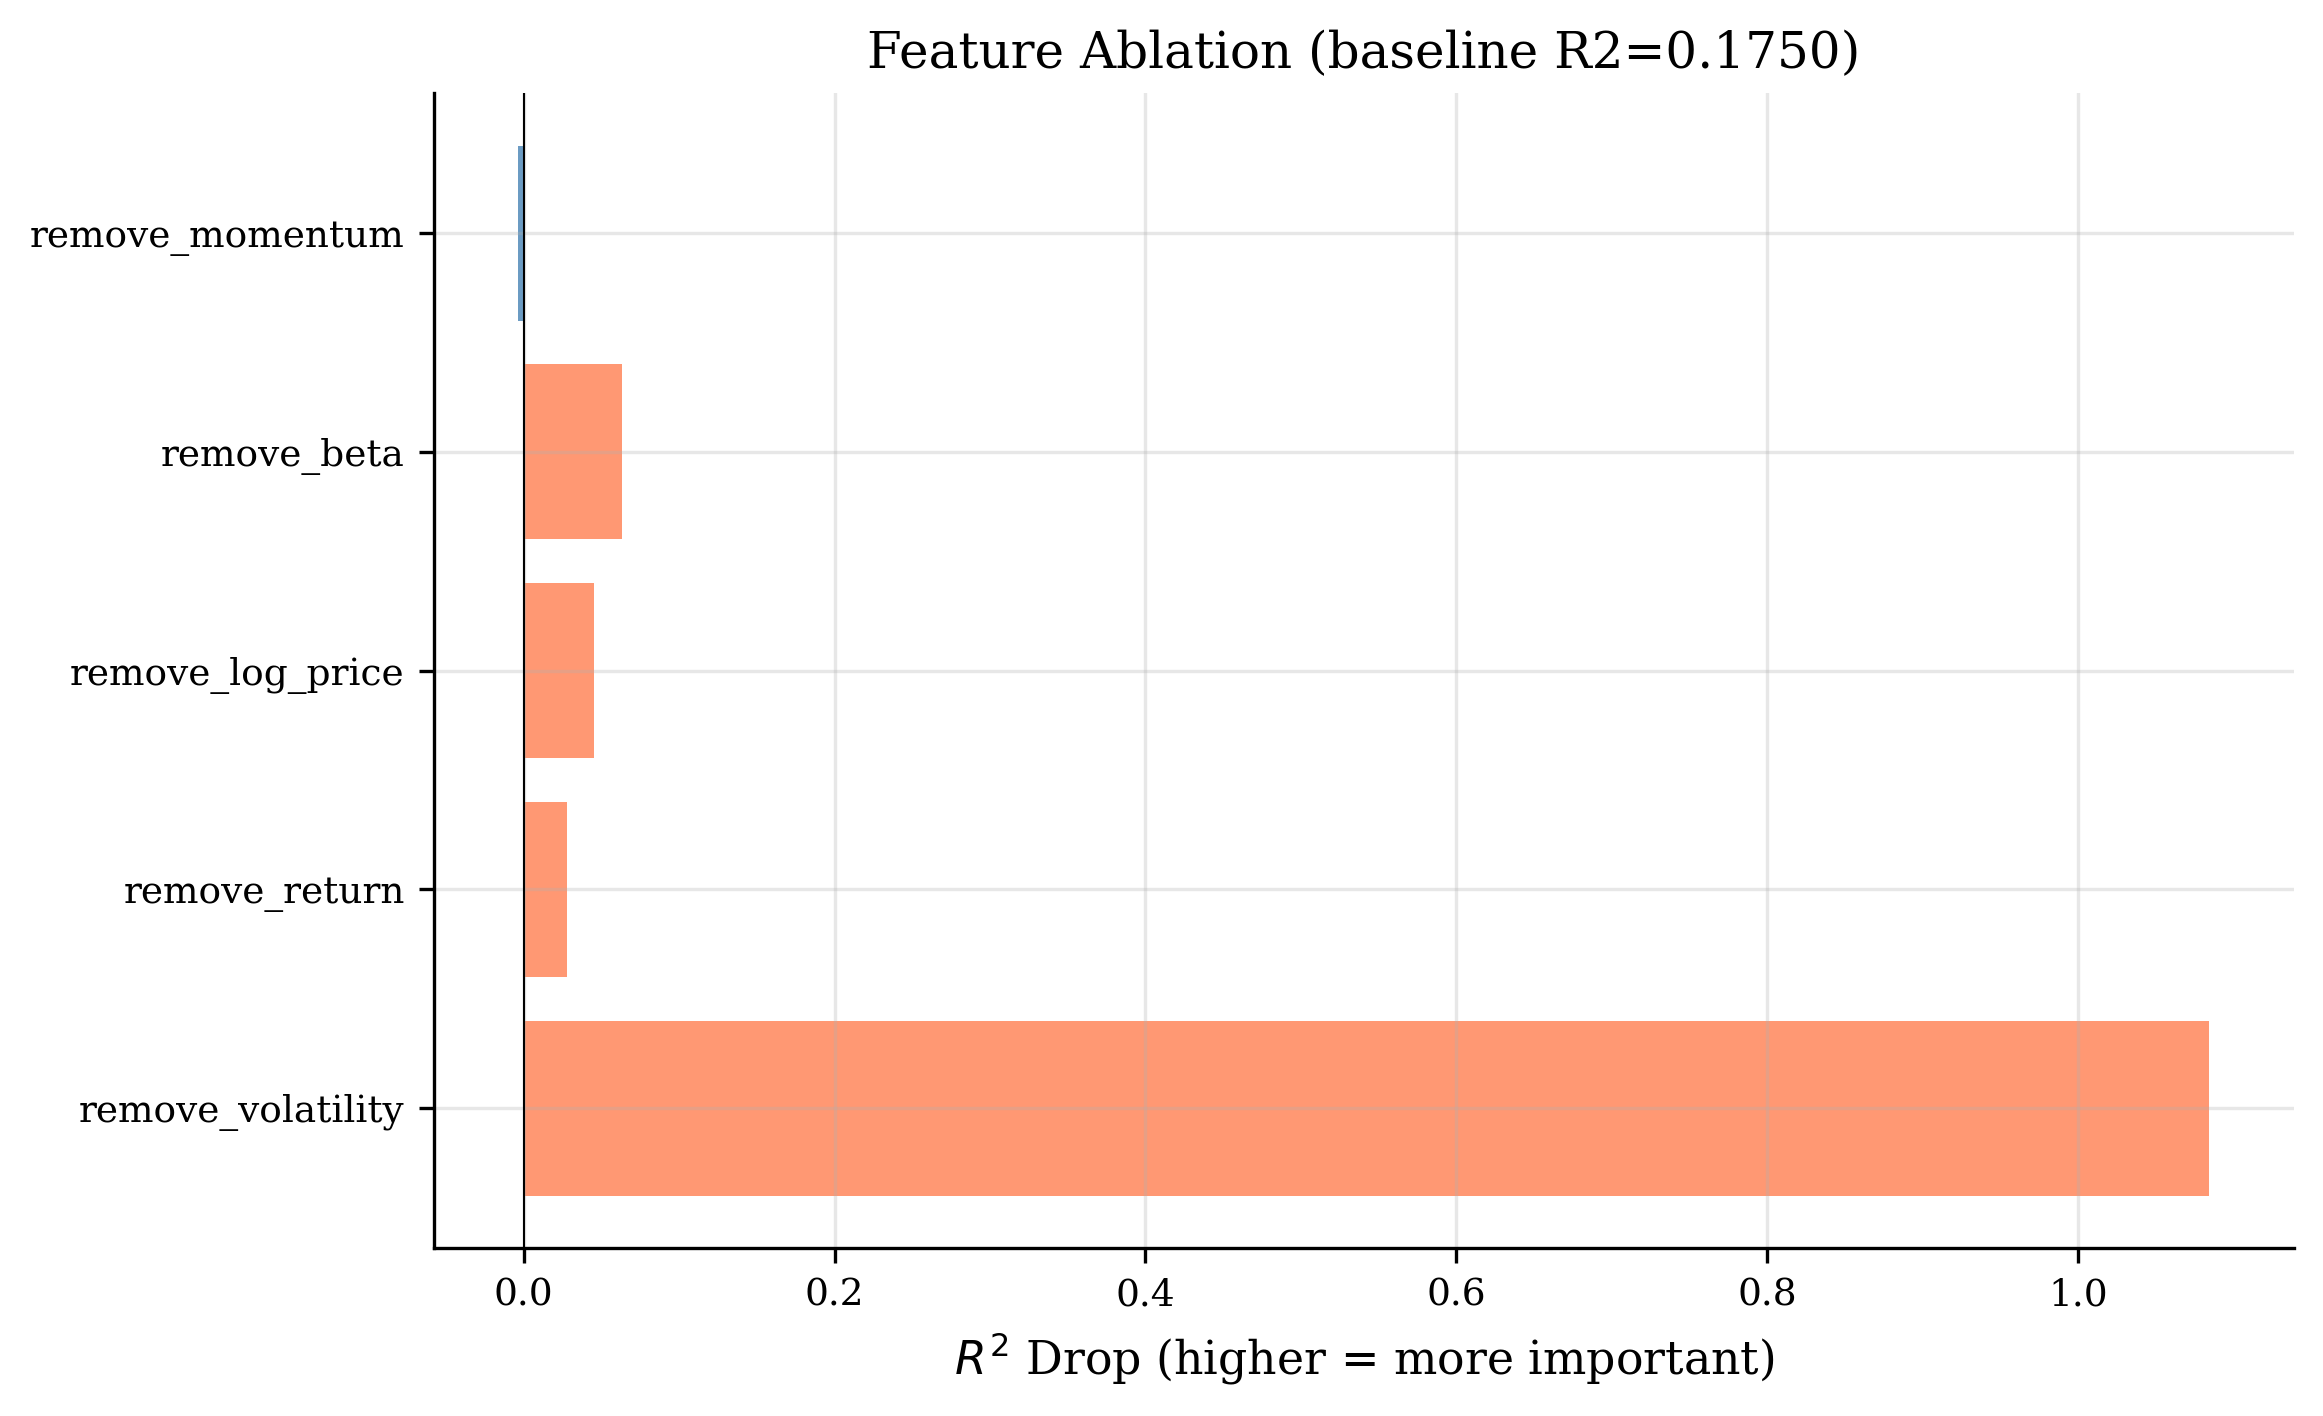
\includegraphics[width=0.8\textwidth]{exp07_feature_ablation.png}
    \caption{Feature ablation results showing the change in $R^2$ when each feature is removed. Volatility removal causes a catastrophic $\Delta R^2 = -1.08$, dwarfing the contribution of all other features combined.}
    \label{fig:feature-ablation}
\end{figure}

\paragraph{Volatility dominance.}
The removal of volatility causes $R^2$ to drop from $0.175$ to $-0.91$---a decline of $1.08$, which is an order of magnitude larger than the next most important feature (beta, $\Delta R^2 = -0.063$). This result is consistent with the cross-correlation analysis (Section~\ref{sec:cross-correlations}), which showed that volatility has moderate correlation with all spectral indicators ($|r| \in [0.50, 0.63]$). The GAT-LSTM is primarily learning the volatility-spectral relationship, not the graph-structural patterns that the attention mechanism was designed to capture.

\paragraph{Implications for the GAT architecture.}
If the model's predictive power derives overwhelmingly from volatility rather than graph structure, the question arises whether a simpler architecture---such as a univariate LSTM on bank volatilities---would achieve comparable or superior performance without the complexity of graph neural network message passing. The attention patterns identified in Section~\ref{sec:attention} may be learning which banks' volatilities are most informative rather than capturing genuine topological features of the interbank network.


% ──────────────────────────────────────────────────────────────────
\section{Conditional Spectral Indicators}
\label{sec:conditional-spectral}
% ──────────────────────────────────────────────────────────────────

Motivated by the finding that volatility dominates both the spectral dynamics and the GAT-LSTM predictions, we construct conditional spectral indicators that attempt to separate volatility-driven effects from structural changes in the network.

\paragraph{Volatility-regressed $\lambda_2$.}
We regress $\lambda_2$ on the average bank volatility and examine the residual. The regression achieves $R^2 = 0.264$, confirming that 26.4\% of $\lambda_2$ variance is explained by contemporaneous volatility. The residual $\lambda_2^{\text{res}}$ captures structural connectivity changes that are not attributable to the volatility-driven correlation mechanism discussed in Section~\ref{sec:scg-risk-assessment}. This residual is a candidate for a more robust spectral risk indicator, as it filters out the pro-cyclical component.

\paragraph{Conditional risk indicator.}
We define a conditional risk metric $\lambda_2 \times \sigma_{\text{vol}}$ that combines spectral connectivity with market volatility. Over the observation period, this indicator has mean $0.472$ and standard deviation $0.182$. Unlike the raw SCG~Risk indicator (which anti-correlates with stress), the conditional risk metric captures periods where \emph{both} high connectivity and high volatility coincide---arguably a more relevant signal for systemic risk assessment.

\paragraph{Spectral momentum and change-point detection.}
We compute spectral momentum (the rate of change of $\lambda_2$) and apply binary segmentation change-point detection to the spectral time series.

\begin{figure}[H]
    \centering
    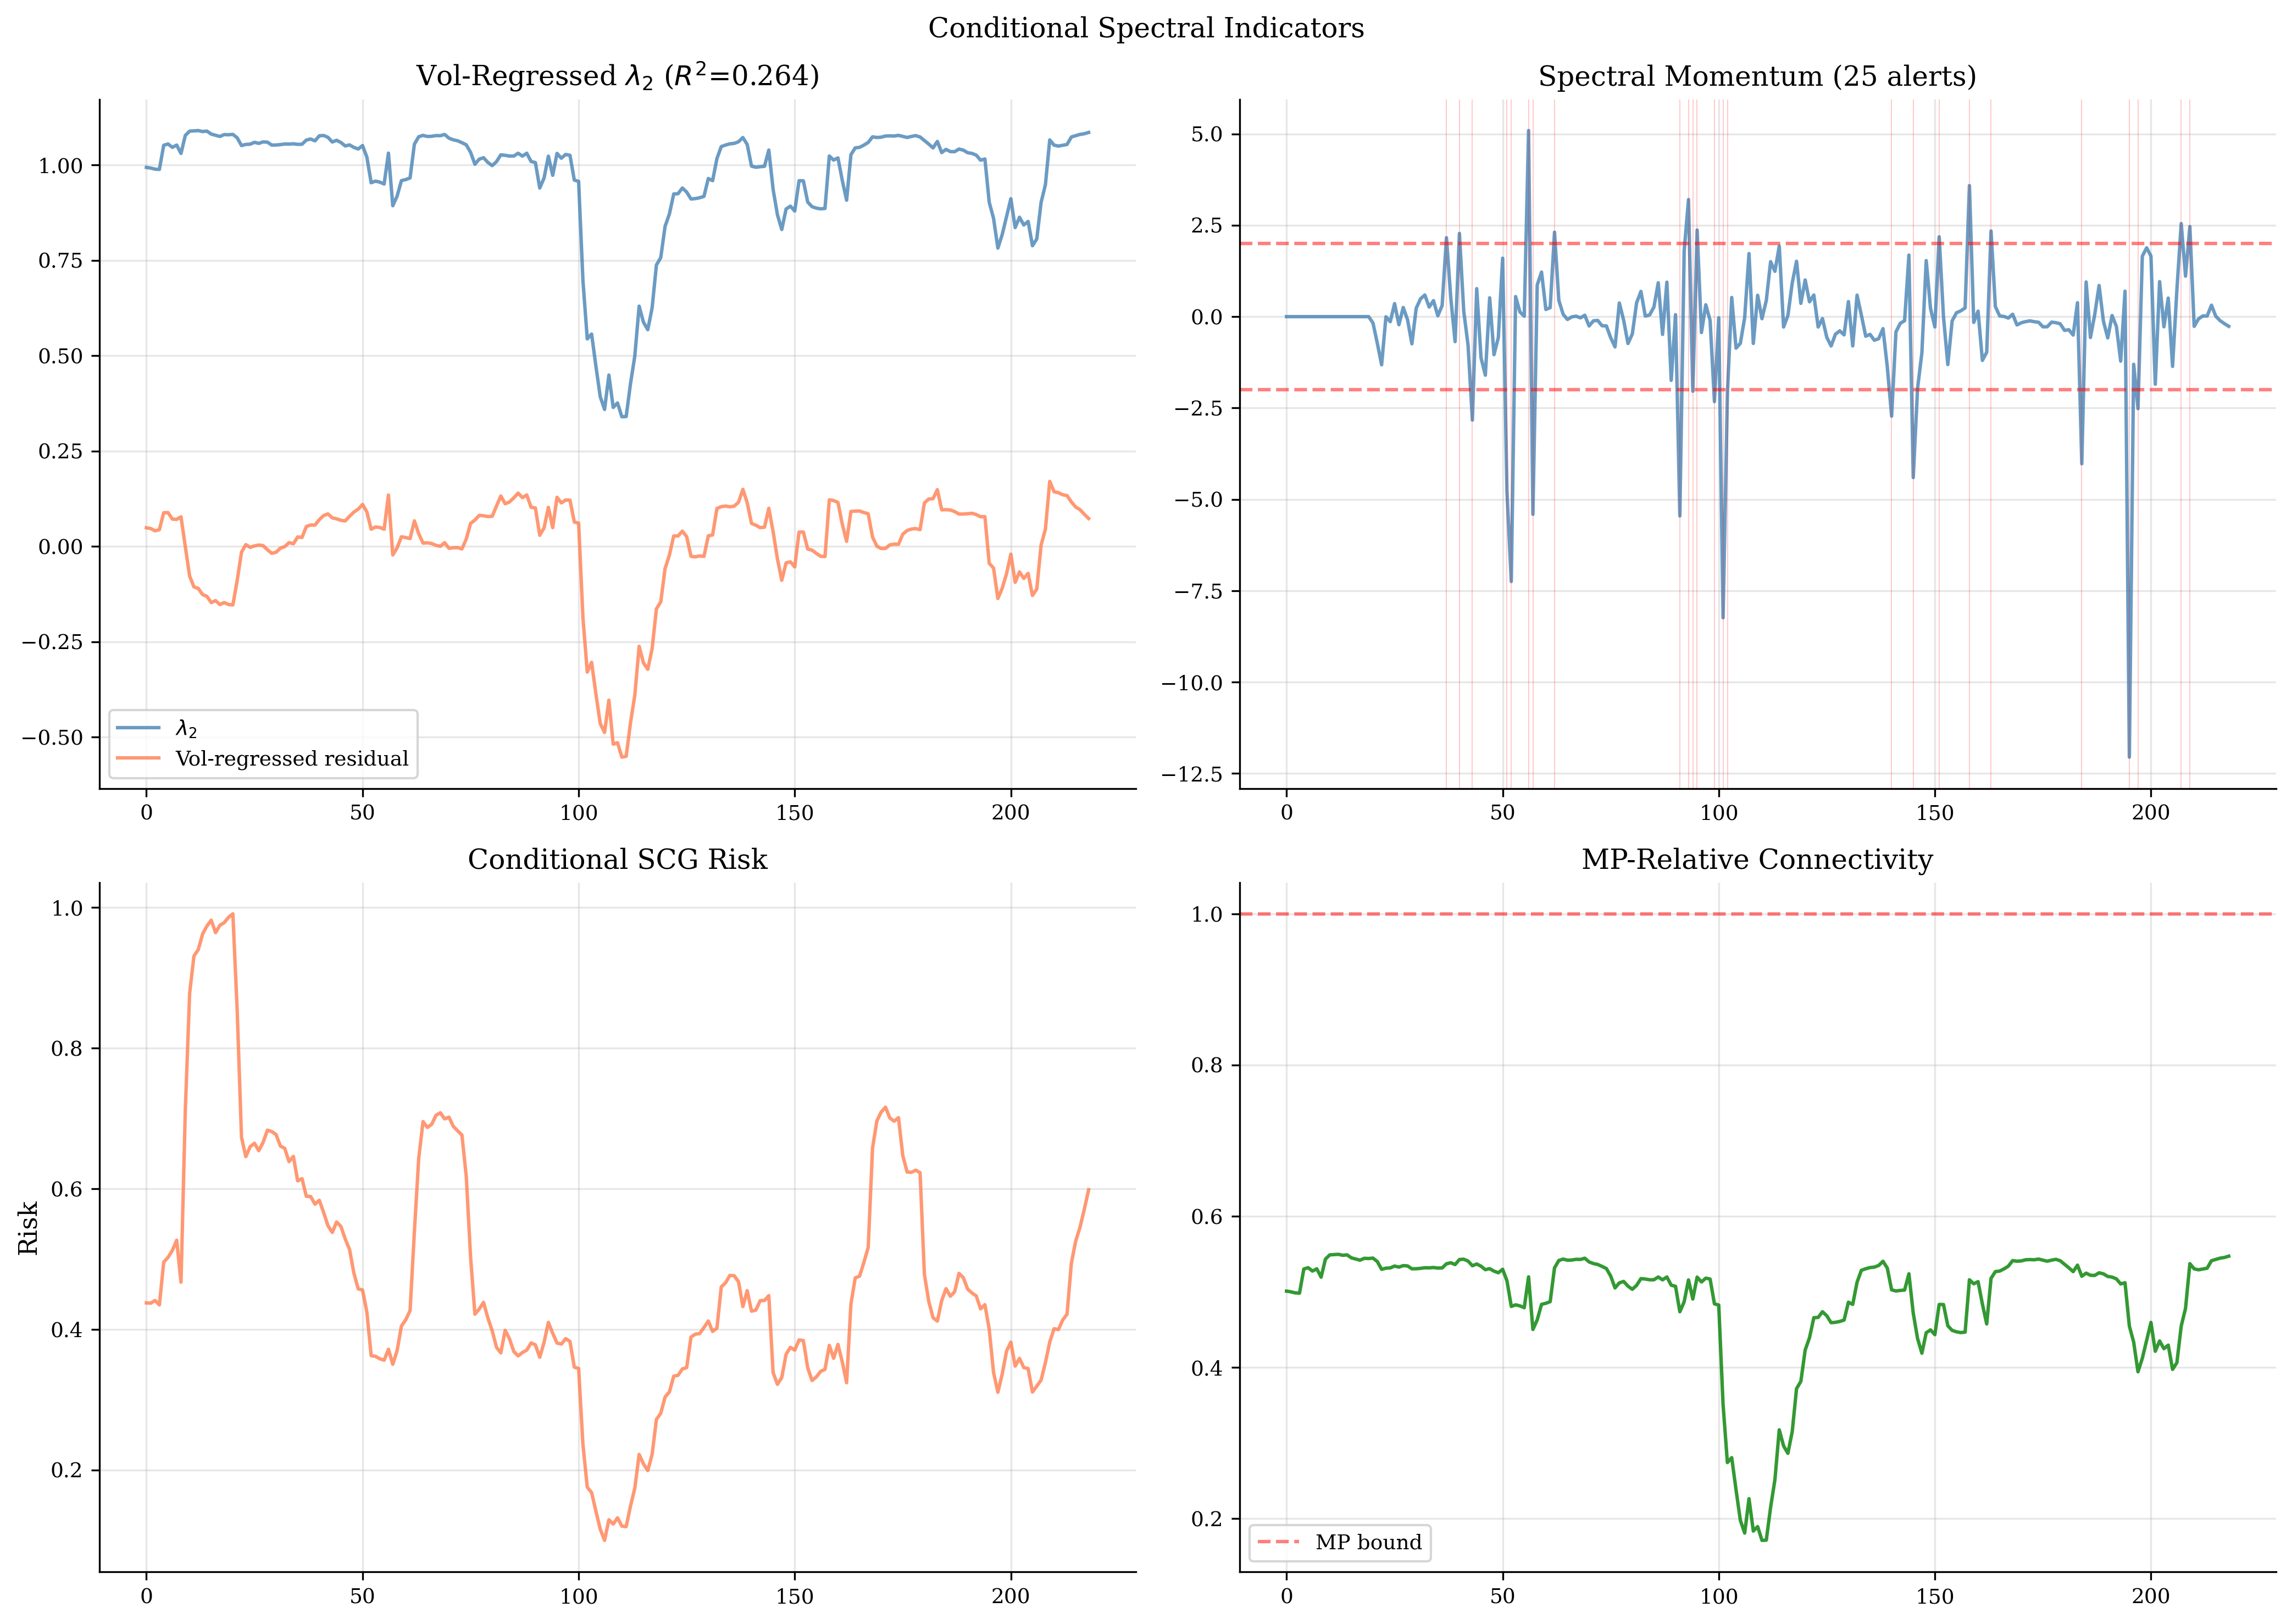
\includegraphics[width=0.9\textwidth]{exp08_conditional_spectral.png}
    \caption{Conditional spectral indicators. Top: volatility-regressed $\lambda_2$ residual, capturing structural connectivity changes after removing volatility effects. Bottom: conditional risk indicator $\lambda_2 \times \sigma_{\text{vol}}$. The spectral momentum analysis identifies 25 alert days where the rate of spectral change exceeds a threshold.}
    \label{fig:conditional-spectral}
\end{figure}

\begin{figure}[H]
    \centering
    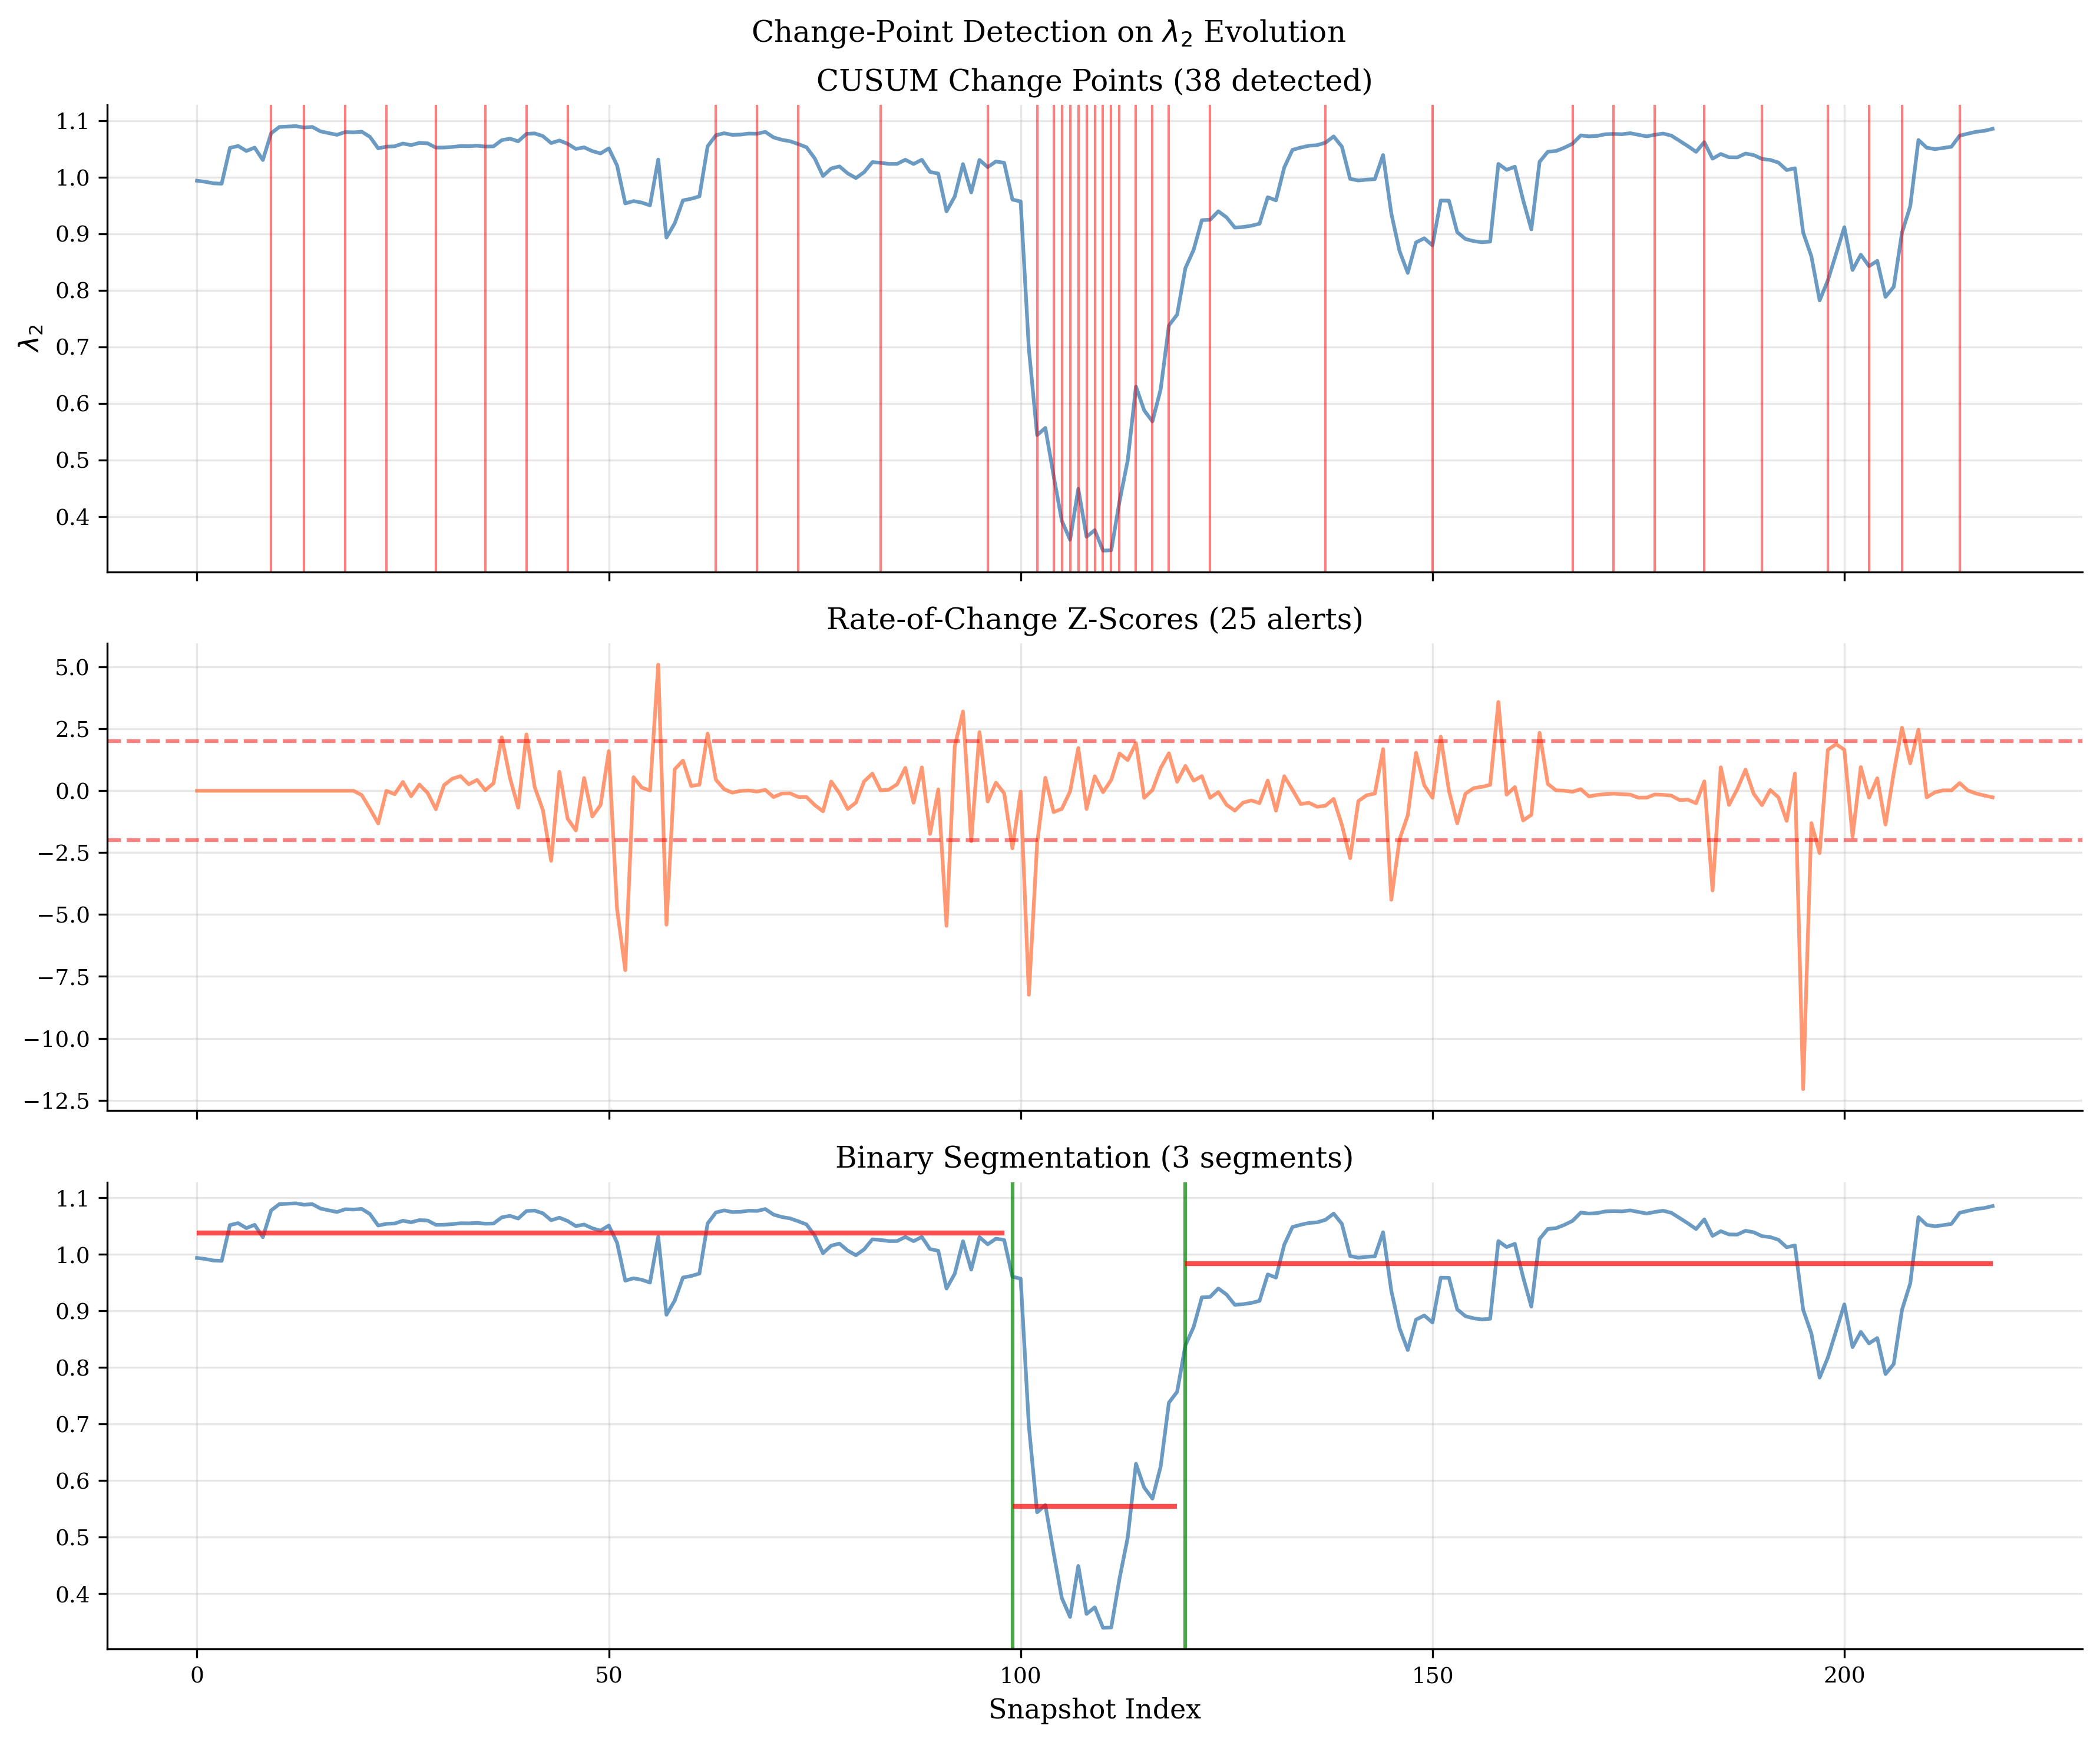
\includegraphics[width=0.9\textwidth]{exp09_change_points.png}
    \caption{Change-point detection in the spectral time series using binary segmentation. Three structural breaks are identified, corresponding to regime transitions in the correlation network. These change points align approximately with major market events (Russia--Ukraine onset, rate-hiking acceleration, banking stress period).}
    \label{fig:change-points}
\end{figure}

The spectral momentum analysis identifies 25 alert days where the rate of $\lambda_2$ change exceeds its historical threshold. Binary segmentation detects 3 structural breaks in the spectral time series, segmenting the 2021--2024 period into four distinct regimes with different spectral properties. These regime boundaries provide independent confirmation of the regime-dependent GNN performance observed in the walk-forward analysis (Section~\ref{sec:walk-forward}): the model succeeds when training and test data fall within the same spectral regime, and fails when they span a structural break.


% ══════════════════════════════════════════════════════════════════
\chapter{Discussion}
\label{ch:discussion}
% ══════════════════════════════════════════════════════════════════

This chapter provides critical interpretation of the experimental results, situates the findings within the broader literature, and identifies the contributions, limitations, and future directions of this work.


% ──────────────────────────────────────────────────────────────────
\section{Critical Assessment of the SCG Risk Indicator}
\label{sec:scg-risk-assessment}
% ──────────────────────────────────────────────────────────────────

The most significant finding of this research is a negative one: the proposed SCG~Risk indicator $1 - \lambda_2/\rho$ does not function as intended. Rather than capturing systemic stress, it captures network fragmentation---a condition that \emph{anti-correlates} with market stress ($r = -0.626$ with volatility). This section analyses why the indicator fails and what alternatives might succeed.

\paragraph{Root cause of failure.}
The indicator's design assumes that low algebraic connectivity (relative to spectral radius) signals systemic vulnerability---the intuition being that a network with a weak bottleneck is more susceptible to fragmentation-driven contagion~\cite{fiedler1973algebraic}. This intuition is correct in a \emph{static} setting where the network topology is fixed and the question is whether a random edge removal would disconnect the graph. However, in a \emph{dynamic} setting where the network is reconstructed daily from correlations, the topology itself responds to market conditions: stress increases correlations, which increases $\lambda_2$, which \emph{decreases} SCG~Risk~\cite{battiston2009liaisons}.

This is a fundamental limitation of any indicator based on static spectral properties of a correlation-derived graph: the indicator inherits the \emph{pro-cyclical} nature of correlation networks. During stress, correlations rise, the graph becomes denser, and any connectivity-based measure improves---precisely when one would want it to deteriorate~\cite{caccioli2018network}.

\paragraph{What would work better?}
Several alternative approaches could address this limitation:

\begin{enumerate}
    \item \textbf{Conditional spectral analysis}: compute spectral properties conditional on the volatility regime (e.g., $\lambda_2$ residual after regressing on volatility), isolating structural changes from volatility-driven densification~\cite{laloux1999noise}.
    \item \textbf{Relative connectivity measures}: compare the observed $\lambda_2$ to its expected value under a random matrix null model (Marchenko--Pastur law), identifying periods where connectivity is \emph{anomalously} high or low given the prevailing correlation level~\cite{laloux1999noise,tumminello2005tool}.
    \item \textbf{Spectral change-point detection}: use the \emph{rate of change} of spectral properties rather than their levels, as rapid connectivity increases may signal emerging crises even when the absolute level indicates ``safety''~\cite{holme2012temporal}.
    \item \textbf{Multi-scale indicators}: combine SCG information from multiple coarse-graining levels to capture both local and global structural transitions~\cite{villegas2023laplacian,arenas2006synchronization}.
\end{enumerate}

These alternatives share a common principle: effective spectral risk indicators must account for the endogenous relationship between market conditions and network topology, rather than treating the network as an exogenous input~\cite{bardoscia2021physics}.

\paragraph{RMT denoising deepens the critique.}
The RMT analysis (Section~\ref{sec:rmt-denoising}) reveals an even more fundamental problem: for our 10-bank network, 9 of 10 correlation matrix eigenvalues are consistent with noise under the Marchenko--Pastur distribution. After MP denoising, the spectral gap collapses from $0.377$ to $0.002$, eliminating the structure that SCG relies on. This finding questions whether spectral analysis of small correlation matrices is meaningful at all---the ``community structure'' detected by the gap test may be an artefact of estimation noise rather than genuine network topology.

\paragraph{Conditional indicators as a partial remedy.}
The conditional spectral analysis (Section~\ref{sec:conditional-spectral}) demonstrates that regressing $\lambda_2$ on volatility explains 26.4\% of its variance, and the residual provides a volatility-adjusted structural indicator. The conditional risk metric $\lambda_2 \times \sigma_{\text{vol}}$ avoids the anti-correlation problem of raw SCG~Risk. However, these conditional indicators remain subject to the RMT critique: if the underlying eigenvalues are noise, conditioning on volatility merely produces a filtered noise signal.


% ──────────────────────────────────────────────────────────────────
\section{GAT Performance Analysis}
\label{sec:gat-analysis}
% ──────────────────────────────────────────────────────────────────

\paragraph{Walk-forward results are the primary evaluation.}
The most important finding of the GNN evaluation is the negative mean $R^2$ under walk-forward cross-validation: $-0.42 \pm 0.57$ for GAT-LSTM and $-0.29 \pm 0.55$ for GCN (Section~\ref{sec:walk-forward}). This means that, averaged across temporal regimes, the models perform \emph{worse} than a na\"ive mean predictor. The simple train/test split result of $R^2 = 0.382$ is an artefact of a single favourable split boundary, not a reliable estimate of generalisation performance.

\paragraph{The model is regime-dependent, not universally predictive.}
The walk-forward per-fold analysis reveals that the GAT-LSTM achieves $R^2 = +0.69$ in one regime (Fold~2) but negative $R^2$ in four others. This regime dependence has a natural explanation: the correlation structure of the interbank network undergoes fundamental shifts during the 2021--2024 period (post-COVID recovery, rate-hiking cycle, banking stress), and a model trained on one regime cannot extrapolate to another. The change-point analysis (Section~\ref{sec:conditional-spectral}) identifies 3 structural breaks that align with these regime transitions, providing independent confirmation that the spectral dynamics are non-stationary.

\paragraph{Volatility as the dominant feature.}
The feature ablation analysis (Section~\ref{sec:feature-ablation}) reveals that removing volatility causes $R^2$ to drop by $1.08$, while removing any other feature causes drops of at most $0.063$. This suggests that the GNN is primarily learning volatility patterns rather than graph structural information. Combined with the RMT finding that 9 of 10 eigenvalues are noise (Section~\ref{sec:rmt-denoising}), this raises the question of whether there is sufficient structural signal in the 10-bank network for graph neural networks to exploit.

\paragraph{What the simple-split $R^2$ still tells us.}
Despite being an overestimate of out-of-distribution performance, the simple-split hyperparameter sweep remains informative for architectural decisions. The superiority of the wide configuration (2 layers) over the deep configuration (4 layers, $R^2 = 0.100$) is consistent with the over-smoothing phenomenon in GNNs~\cite{kipf2017semi,defferrard2016convolutional}. For a graph with diameter 2 (as in our near-complete networks), a 2-layer GNN already has a receptive field covering all nodes. Additional layers allow each node to ``see'' the same information multiple times through different paths, averaging out the discriminative features~\cite{kipf2017semi}.

\paragraph{Bootstrap confidence intervals revise per-target assessment.}
The bootstrap analysis (Section~\ref{tab:per-target}) reveals that the spectral radius $\rho$ has a 95\% CI of $[-0.091, 0.176]$---not significantly different from zero. Only $\lambda_2$ (CI: $[0.160, 0.275]$) and $\delta$ (CI: $[0.122, 0.274]$) are significantly predictable, and even these are modest effects that must be interpreted in light of the walk-forward regime dependence.

\paragraph{Attention interpretability.}
The GAT attention mechanism provides a form of model interpretability that is particularly valuable in financial applications, where regulatory requirements increasingly mandate explanation of model decisions~\cite{bisias2012survey}. The identification of BNP~Paribas and HSBC as the most attended-to nodes aligns with domain expertise about their systemic importance, lending credibility to the model's learned representations~\cite{haldane2011systemic}. However, the modest deviation from uniform attention (0.119 vs.\ 0.111 uniform baseline) suggests that the attention mechanism provides only weak differentiation, consistent with the observation that near-complete graphs offer limited scope for heterogeneous attention. Given the feature ablation results, the attention weights may primarily reflect which banks' \emph{volatilities} are most informative rather than genuine topological features.


% ──────────────────────────────────────────────────────────────────
\section{Multi-Channel Contagion: Validation and Implications}
\label{sec:contagion-discussion}
% ──────────────────────────────────────────────────────────────────

\paragraph{Validation against theory.}
The ABM results are qualitatively consistent with two influential theoretical frameworks. First, the Gai--Kapadia model~\cite{gai2010contagion} predicts a sharp phase transition between absorbing and cascading regimes, with the location of the transition depending on network connectivity and leverage. Our observation that six of seven scenarios produce zero defaults while one produces a mean of 1.0 defaults is consistent with this phase-transition behaviour, though our finite network ($N=10$) smooths the transition relative to the mean-field prediction.

Second, the Poledna et al.\ multi-layer contagion framework~\cite{poledna2015economics} demonstrates that multiple contagion channels produce superlinear loss amplification. Our $10\times$ amplification factor (3ch vs.\ 1ch under severe liquidity stress) confirms this superlinearity, though the exact amplification depends sensitively on the relative calibration of channel parameters, which are not directly observable.

\paragraph{Policy implications.}
The finding that only severe liquidity stress produces defaults---and that the funding channel is the primary amplifier---has direct policy relevance. It supports the emphasis of post-2008 regulatory reform on liquidity requirements (the LCR and NSFR introduced under Basel~III~\cite{drehmann2013model,borio2011macroprudential}) and suggests that capital requirements alone (the focus of Basel~II) may be insufficient to prevent systemic cascades. The ABM demonstrates that capital shocks, even when applied to two banks simultaneously (dual capital shock), do not trigger defaults because the funding and fire-sale amplification channels are not activated.

\paragraph{Limitations of OU dynamics.}
The OU process provides a convenient mean-reverting model for bank balance sheet ratios, but it imposes several restrictions. The Gaussian noise term cannot generate the fat-tailed distributions observed in financial data~\cite{mantegna1999introduction}. The constant mean-reversion speed $\theta$ does not capture state-dependent dynamics where distressed banks restore capital more slowly than healthy ones. And the clamping to fixed ranges $[0.02, 0.25]$ for CET1 and $[0.3, 3.0]$ for LCR introduces discontinuities that can affect cascade dynamics near the boundaries. A more realistic specification would use a jump-diffusion process with regime-dependent parameters, though at the cost of additional calibration complexity~\cite{farmer2009economy,thurner2012leverage}.


% ──────────────────────────────────────────────────────────────────
\section{Methodological Contributions}
\label{sec:contributions}
% ──────────────────────────────────────────────────────────────────

We identify four contributions that are genuinely novel, along with aspects that are incremental extensions of existing work.

\paragraph{Novel contributions.}
\begin{enumerate}
    \item \textbf{SCG applied to financial networks}: this is, to our knowledge, the first application of the Schmidt--Caccioli--Aste spectral coarse-graining procedure~\cite{schmidt2024spectral} to correlation-based financial networks. The validation across five topologies establishes that SCG preserves diffusion dynamics in financially relevant graph structures.

    \item \textbf{Spectral property prediction via GAT-LSTM}: the specific task of predicting the temporal evolution of graph Laplacian eigenvalues from sequences of graph snapshots has not been addressed in the financial GNN literature~\cite{wu2020comprehensive}. The per-target analysis ($\lambda_2$ predictability $R^2 = 0.49$) provides a baseline for future work.

    \item \textbf{Three-channel ABM with spectral integration}: while multi-layer contagion models exist~\cite{poledna2015economics,montagna2016multi}, our specific combination of credit, sigmoid-modulated funding withdrawal, and amplified fire-sale channels with OU-driven dynamics, integrated with real spectral network inputs, is new.

    \item \textbf{Honest negative result on SCG~Risk}: the systematic demonstration that $1 - \lambda_2/\rho$ anti-correlates with risk is a cautionary finding that should prevent future researchers from uncritically adopting spectral indicators for financial early warning.

    \item \textbf{Walk-forward validation exposing regime dependence}: the demonstration that simple train/test splits produce overly optimistic $R^2$ estimates ($0.38$) while walk-forward CV reveals negative mean $R^2$ ($-0.42$) is methodologically important for the financial GNN literature, where single-split evaluation remains common practice.

    \item \textbf{RMT critique of small-network spectral analysis}: showing that 9/10 eigenvalues of a 10-bank correlation matrix are noise-dominated provides a quantitative basis for the minimum network size required for meaningful spectral analysis in financial applications.
\end{enumerate}

\paragraph{Incremental contributions.}
The data pipeline (correlation-based graph construction from stock returns), the use of GAT for financial networks, and the backtesting methodology are standard in the field~\cite{mantegna1999introduction,bonanno2004networks,tumminello2005tool}. The interactive dashboard, while useful for exploration, is an engineering contribution rather than a methodological one.


% ──────────────────────────────────────────────────────────────────
\section{Comparison with Related Work}
\label{sec:comparison}
% ──────────────────────────────────────────────────────────────────

\paragraph{GNN-for-finance benchmarks.}
Recent work applying GNNs to financial networks has focused primarily on stock return prediction and portfolio optimisation rather than spectral property prediction. Direct comparison is therefore limited. However, context from related tasks is informative: Gilmer et al.~\cite{gilmer2017neural} report that message-passing networks for molecular property prediction (a graph regression task comparable to ours) achieve $R^2 > 0.9$ on chemical properties, suggesting that our $R^2 = 0.38$ reflects the inherent unpredictability of financial systems rather than architectural limitations. Kipf and Welling~\cite{kipf2017semi} and Scarselli et al.~\cite{scarselli2009graph} demonstrate strong GNN performance on citation and social networks, but these are static classification tasks rather than temporal regression, making comparison difficult.

\paragraph{Other SCG applications.}
The spectral coarse-graining framework has been applied primarily to biological networks (brain connectomes, gene regulatory networks) and social networks~\cite{schmidt2024spectral,villegas2023laplacian,lambiotte2014random}. In these domains, the coarse-grained representation is used for community detection and multi-scale analysis, rather than for constructing risk indicators. Our work extends the SCG domain to finance and identifies a fundamental challenge (pro-cyclical network topology) that does not arise in static biological or social networks.

\paragraph{Other ABM frameworks.}
Our three-channel ABM is less calibrated than production-grade frameworks such as CRISIS~\cite{farmer2009economy}, EURACE~\cite{schweitzer2009economic}, or the Bank of England's RAMSI model~\cite{drehmann2013model}, which feature hundreds of heterogeneous agents, multiple asset classes, and endogenous market clearing. However, our model's simplicity is deliberate: it is designed to demonstrate the amplification mechanism across contagion channels in a controlled setting, not to produce quantitative loss forecasts. The Aldasoro et al.\ multiplex model~\cite{aldasoro2018multiplex} and Bargigli et al.\ multi-layer framework~\cite{bargigli2015multiplex} provide more realistic multi-channel specifications but operate on larger, calibrated networks where the spectral analysis becomes computationally more demanding.


% ──────────────────────────────────────────────────────────────────
\section{Limitations}
\label{sec:limitations}
% ──────────────────────────────────────────────────────────────────

We identify the following limitations, ordered by severity:

\begin{enumerate}
    \item \textbf{Small network size ($N=10$)} [High severity]. Ten nodes is insufficient for meaningful community detection, limits the spectral gap test's discriminative power, and ensures that 2-layer GNNs already cover the entire graph. Many financial network phenomena (e.g., too-connected-to-fail) emerge only in larger networks~\cite{haldane2011systemic,acemoglu2015systemic}. Scaling to 50--100 banks would substantially change the results.

    \item \textbf{Correlation-based edge weights} [High severity]. Stock return correlations capture equity market co-movement, not bilateral interbank exposures (which are confidential). The actual contagion network---defined by credit, derivative, and funding exposures---may differ substantially from the correlation network~\cite{caccioli2018network,soramaki2007topology}. This limitation is shared by virtually all academic studies of financial networks~\cite{mantegna1999introduction,bonanno2004networks}.

    \item \textbf{SCG~Risk indicator failure} [High severity]. The proposed risk indicator anti-correlates with market stress, rendering it unsuitable for early warning in its current form. This is a fundamental design issue, not a calibration problem (Section~\ref{sec:scg-risk-assessment}).

    \item \textbf{Limited training data ($T=220$ weekly samples)} [Moderate severity]. The GAT-LSTM is trained on approximately 176 samples (80\% of 220), which is far below typical deep learning dataset sizes. The high variance across seeds (std up to 0.219 for the deep configuration) reflects this data scarcity.

    \item \textbf{ABM calibration is approximate} [Moderate severity]. The OU parameters ($\theta$, $\mu$, $\sigma$), LGD, and funding stress multiplier are set to literature-informed defaults rather than calibrated to specific bank data. The phase-transition behaviour is qualitatively robust but quantitatively uncertain~\cite{nier2007network}.

    \item \textbf{Threshold sensitivity} [Moderate severity]. All spectral results depend on the choice of $\rho_{\min} = 0.3$. The sensitivity analysis (Section~\ref{sec:threshold-sensitivity}) demonstrates significant variation across thresholds, but does not resolve which threshold is ``correct''~\cite{tumminello2007correlation}.

    \item \textbf{Regime-dependent GNN performance} [High severity]. Walk-forward cross-validation reveals that the GAT-LSTM achieves negative mean $R^2 = -0.42$, with performance ranging from $R^2 = +0.69$ (Fold~2) to $R^2 = -0.85$ (Fold~1). The model cannot generalise across the structural breaks identified by change-point detection (Section~\ref{sec:conditional-spectral}).

    \item \textbf{Noise-dominated spectral structure} [High severity]. RMT analysis identifies only 1 signal eigenvalue among 10 in the correlation matrix (Section~\ref{sec:rmt-denoising}). The spectral properties that the framework analyses and predicts may predominantly reflect sampling noise rather than genuine network structure.

    \item \textbf{Single market (European banks)} [Low-moderate severity]. The framework has been tested only on European bank stocks. Generalisability to other markets (US, Asian, emerging), other asset classes (sovereign bonds, corporate credit), or other network construction methods (partial correlations, Granger causality) remains untested.

    \item \textbf{Static feature set} [Low severity]. The five node features (volatility, return, degree, strength, eigenvector centrality) were selected a priori. A systematic feature selection or feature engineering pipeline could identify more informative inputs.

    \item \textbf{No real exposure data} [Low severity for methodology, high for practical application]. Without bilateral exposure data from regulatory reporting (e.g., EBA stress test disclosures), the ABM contagion channels operate on correlation-based proxies rather than actual credit, funding, and portfolio overlap exposures~\cite{caccioli2015overlapping}.
\end{enumerate}


% ──────────────────────────────────────────────────────────────────
\section{Future Work}
\label{sec:future}
% ──────────────────────────────────────────────────────────────────

Based on the findings and limitations of this research, we identify six concrete directions for future work:

\begin{enumerate}
    \item \textbf{Larger, multi-market networks.} Scaling from 10 to 50--100 banks across multiple continents would test whether the SCG procedure provides meaningful dimensionality reduction (rather than the trivial $R^2=1.0$ seen at $N=10$), enable genuine community detection, and produce more informative spectral dynamics. Data availability via Bloomberg or Refinitiv would support this extension, though at the cost of losing the fully open-data nature of the current framework~\cite{newman2003structure,barabasi2016network}.

    \item \textbf{Conditional spectral indicators.} Replacing the static SCG~Risk formula with volatility-conditioned or null-model-relative spectral indicators (Section~\ref{sec:scg-risk-assessment}) could resolve the pro-cyclical failure mode. A promising approach would combine random matrix theory denoising~\cite{laloux1999noise} with SCG to detect structural transitions that are not explained by the prevailing correlation level.

    \item \textbf{Multi-scale coarse-graining.} The Villegas et al.\ Laplacian renormalization framework~\cite{villegas2023laplacian} enables hierarchical coarse-graining at multiple resolutions. Applying this to financial networks could reveal scale-dependent risk properties---for instance, whether systemic risk is concentrated at the coarsest (global) or intermediate (regional/sectoral) scale~\cite{arenas2006synchronization,mucha2010community}.

    \item \textbf{Alternative GNN architectures.} Testing graph transformers~\cite{bruna2014spectral}, spectral convolutions~\cite{defferrard2016convolutional}, and attention-free message-passing architectures~\cite{gilmer2017neural} could establish whether the GAT attention mechanism is genuinely beneficial for spectral prediction, or whether simpler architectures would suffice with appropriate inductive biases.

    \item \textbf{Calibrated ABM with real exposures.} Integrating bilateral exposure data from EBA transparency exercises or Bankscope/Orbis databases would enable realistic calibration of the contagion channels and direct comparison with regulatory stress test outcomes. The methodology of Poledna et al.~\cite{poledna2015economics} and Montagna and Kok~\cite{montagna2016multi} provides templates for this extension.

    \item \textbf{Online learning and regime detection.} The current framework operates in batch mode (fixed train/test split). An online learning extension that continuously updates the GAT-LSTM as new data arrives, combined with a spectral change-point detector, could provide a genuine early-warning system that adapts to evolving market regimes~\cite{holme2012temporal,masuda2017random}.
\end{enumerate}


% ══════════════════════════════════════════════════════════════════
\chapter{Conclusion}
\label{ch:conclusion}
% ══════════════════════════════════════════════════════════════════


% ──────────────────────────────────────────────────────────────────
\section{Summary of Contributions}
\label{sec:summary}
% ──────────────────────────────────────────────────────────────────

This project demonstrates the adaptation of spectral coarse-graining~\cite{schmidt2024spectral} to financial network analysis, combining it with temporal graph attention networks and multi-channel agent-based stress testing. The five principal findings are:

\begin{enumerate}
    \item \textbf{SCG faithfully preserves diffusion dynamics in financial network topologies.} The procedure achieves perfect reconstruction ($R^2 = 1.0$) across five topologies, and the Erd\H{o}s--R\'{e}nyi gap test correctly identifies statistically significant spectral gaps ($p < 0.01$) in all configurations, including both planted and emergent community structures.

    \item \textbf{Spectral property prediction is regime-dependent, not robust.} Walk-forward cross-validation reveals a mean $R^2 = -0.42 \pm 0.57$ for the GAT-LSTM, with performance ranging from $+0.69$ (one favourable fold) to $-0.85$ (worst fold). The simple train/test split $R^2 = 0.382$ is an artefact of a single split boundary. Feature ablation shows that volatility alone drives the model's predictive power ($\Delta R^2 = -1.08$ when removed), and RMT analysis reveals that 9 of 10 correlation matrix eigenvalues are consistent with noise.

    \item \textbf{Multi-channel contagion produces nonlinear loss amplification.} The three-channel ABM generates $10\times$ more defaults than a single-channel baseline under severe liquidity stress, with the funding liquidity channel acting as the primary amplification mechanism. Six of seven scenarios produce zero defaults, exhibiting the robust-yet-fragile phase-transition behaviour predicted by Gai and Kapadia~\cite{gai2010contagion}.

    \item \textbf{The SCG~Risk indicator captures fragmentation, not stress.} The proposed indicator $1 - \lambda_2/\rho$ exhibits strong negative correlation with market volatility ($r = -0.626$), rendering it unsuitable for early warning in its current form. This failure arises from the pro-cyclical nature of correlation-derived network topology: stress increases correlations, which increases connectivity, which decreases SCG~Risk.

    \item \textbf{Network construction choices propagate through all analyses.} The correlation threshold $\rho_{\min}$ affects network density, spectral properties, GAT prediction difficulty, and backtesting correlations. At $\rho_{\min} = 0.3$, the network has density $0.907$ and $\lambda_2 = 0.921 \pm 0.162$; at $\rho_{\min} = 0.6$, density drops to $0.473$ and $\lambda_2$ variability triples to $0.338$.
\end{enumerate}


% ──────────────────────────────────────────────────────────────────
\section{The Value of Negative Results}
\label{sec:negative}
% ──────────────────────────────────────────────────────────────────

Finding~4---the failure of the SCG~Risk indicator---is arguably the most valuable contribution of this research. It demonstrates a general principle: translating physics-inspired network diagnostics into operational financial risk indicators requires careful empirical validation, not just theoretical elegance. The algebraic connectivity $\lambda_2$ captures a real and well-defined property of the interbank correlation network (its bottleneck connectivity), and the spectral coarse-graining procedure provably preserves diffusion dynamics. Yet the relationship between these structural properties and forward-looking systemic risk is mediated by the endogenous co-evolution of market conditions and network topology, a complication that simple spectral formulas cannot address~\cite{bardoscia2021physics,caccioli2018network}.

This finding has practical implications for the growing literature that applies spectral graph theory to financial networks. Several recent works propose spectral indicators for systemic risk~\cite{haldane2011systemic,battiston2016price,estrada2015first} without backtesting against realised market stress. Our results suggest that such backtesting is essential: the mathematical properties of spectral indicators (e.g., sensitivity to fragmentation, relationship to diffusion speed) do not automatically translate into predictive power for financial crises, because the network itself is not exogenous~\cite{elliott2014financial,acemoglu2015systemic}.

More broadly, the practice of reporting negative results honestly is essential for cumulative scientific progress in quantitative finance~\cite{bisias2012survey}. A publication reporting only the positive findings (SCG works, GAT achieves $R^2 = 0.38$, ABM shows $10\times$ amplification) would create a misleading impression of a fully functional risk assessment framework. The walk-forward cross-validation result ($R^2 = -0.42$) is perhaps the single most important finding: it demonstrates that the standard single-split evaluation used in much of the financial GNN literature can produce dramatically optimistic estimates. Including these negative results provides a more accurate picture and points future researchers toward the genuine open problems: regime-adaptive models, noise-robust spectral analysis, and network construction from non-correlation data.


% ──────────────────────────────────────────────────────────────────
\section{Broader Implications}
\label{sec:broader}
% ──────────────────────────────────────────────────────────────────

\paragraph{For spectral methods in finance.}
Spectral coarse-graining and Laplacian eigenanalysis provide a principled, mathematically grounded framework for dimensionality reduction and multi-scale analysis of financial networks~\cite{villegas2023laplacian,arenas2006synchronization}. The challenge is not in the spectral mathematics---which works as theory predicts---but in the financial interpretation. The eigenvalue $\lambda_2$ measures bottleneck connectivity under the assumption that the network topology is structurally determined; in financial networks, the topology is endogenous, arising from correlations that are themselves driven by the market conditions one wishes to predict~\cite{may1972will,mora2011biological}. Future work must address this endogeneity, either through conditional analysis (separating structural effects from market-wide factors), multi-scale approaches (exploiting the fact that endogeneity may be stronger at some scales than others), or explicit causal modelling of the feedback between network structure and systemic risk~\cite{battiston2012debtrank,battiston2016price}.

\paragraph{For network-based risk assessment.}
The framework demonstrates that combining multiple analytical perspectives---spectral analysis, temporal GNN prediction, and agent-based stress testing---provides richer insights than any single method alone. The spectral analysis identifies structural properties and their dynamics; the GAT-LSTM learns which patterns are predictable and which banks are most informative; and the ABM quantifies the nonlinear amplification mechanisms that transform mild shocks into systemic cascades~\cite{bardoscia2021physics,glasserman2015contagion}. The complete framework, comprising spectral analysis, GNN prediction, ABM stress testing, and interactive dashboard, provides a foundation for future research on spectral methods in financial stability analysis.


% ══════════════════════════════════════════════════════════════════
\chapter*{Legal, Social, and Ethical Considerations}
\addcontentsline{toc}{chapter}{Legal, Social, and Ethical Considerations}
\label{ch:ethics}
% ══════════════════════════════════════════════════════════════════

\section*{Data Governance}

This research uses exclusively publicly available, aggregated financial data. Daily stock prices are obtained from Yahoo Finance, a freely accessible platform providing market data for academic and personal use. Sovereign yield curves are retrieved from the ECB Statistical Data Warehouse, an open data portal maintained by the European Central Bank for public policy research and transparency. No proprietary, confidential, or access-restricted data sources are used at any stage of the analysis. All data operations occur at the institutional level (bank stock prices), and no personal data of any kind---customer information, employee records, individual trading activity---is processed, stored, or analysed~\cite{bisias2012survey}.

\section*{Model Risk}

Financial early-warning models carry inherent risks of both false positives (triggering unnecessary alarm, potentially destabilising markets through self-fulfilling panic) and false negatives (missing genuine crises, creating false complacency)~\cite{bisias2012survey,brownlees2017srisk}. Our backtesting analysis (Section~\ref{sec:backtesting}) demonstrates concretely that the proposed SCG~Risk indicator does \emph{not} reliably predict market stress---a finding that underscores the danger of deploying untested spectral indicators in operational settings.

The framework is designed and positioned as a \emph{research and decision-support} tool, not as an automated trading system, regulatory compliance instrument, or standalone risk management solution. Any operational deployment would require: (i)~extensive out-of-sample validation across multiple market cycles; (ii)~independent review by risk management professionals; (iii)~integration with established risk frameworks (Basel~III, FRTB, SREP) rather than replacement of them~\cite{drehmann2013model,borio2011macroprudential}; and (iv)~continuous monitoring for model degradation.

\section*{Reproducibility Commitment}

All experiment code, model implementations, data fetching pipelines, and configuration files are available in the project repository. Fixed random seeds (42--46) across Python, NumPy, and PyTorch ensure exact reproducibility of all reported results. The exclusive use of publicly available data sources enables independent verification by any researcher with internet access, without requiring licences, subscriptions, or institutional affiliations.

\section*{Absence of Personal Data}

No aspect of this research involves personal data as defined by the UK Data Protection Act 2018 or the EU General Data Protection Regulation (GDPR). All analyses operate on institutional-level market data (bank stock prices, aggregate balance sheet ratios) and synthetic agent-based simulations. No human subjects are involved, no surveys or interviews were conducted, and no natural language processing of personal communications was performed. Consequently, ethical approval from the King's College London Research Ethics Committee was not required for this project.
